\documentclass[a4paper]{article}
\usepackage[T1]{fontenc}			% pacchetto per \chapter
\usepackage[italian]{babel}
\usepackage[italian]{isodate}  		% formato delle date in italiano
\usepackage{graphicx}				% gestione delle immagini
\usepackage{amsfonts}
\usepackage{booktabs}				% tabelle di qualità superiore
\usepackage{amsmath}				% pacchetto matematica
\usepackage{mathtools}				% per sottolineare sotto le equazioni
\usepackage{stmaryrd} 				% per '\llbracket' e '\rrbracket'
\usepackage{amsthm}					% teoremi migliorati
\usepackage{enumitem}				% gestione delle liste
\usepackage{pifont}					% pacchetto con elenchi carini
\usepackage{enumitem}				% pacchetto per elenchi con lettere dell'alfabeto
\usepackage{cancel}					% per cancellare delle espressioni matematiche


\usepackage[x11names]{xcolor}		% pacchetto colori RGB
% Link ipertestuali per l'indice
\usepackage{xcolor}
\usepackage[linkcolor=black, citecolor=blue, urlcolor=cyan]{hyperref}
\hypersetup{
	colorlinks=true
}

%\usepackage{showframe}				% visualizzazione bordi
%\usepackage{showkeys}				% visualizzazione etichetta

\newtheorem{theorem}{\textcolor{Red3}{\underline{Teorema}}}
\newtheorem{lemma}{Lemma}
\renewcommand{\qedsymbol}{QED}
\newcommand{\exec}[1]{\llbracket #1\:\rrbracket}
\newcommand{\dquotes}[1]{``#1''}
\newcommand{\longline}{\noindent\rule{\textwidth}{0.4pt}}

\begin{document}
	\author{VR443470}
	\title{Fondamenti dell'informatica}
	\date{\printdayoff\today}
	\maketitle
	
	\newpage
	
	% indice
	\tableofcontents
	
	\newpage
	
	\section{Introduzione alla materia}
	
	Prima di iniziare con la presentazione di alcuni concetti fondamentali, si definisce l'\textbf{invariante induttiva}: pensando a qualsiasi linguaggio di programmazione, una generica condizione è \underline{sempre} vera prima, durante e dopo un ciclo. Questo concetto ritornerà in futuro.
	
	\subsection{Cardinalità degli insiemi}
	Il motivo dell'interesse di un ripasso di un argomento trattato in passato è giustificato dal fatto che i dati manipolati in informatica sono (e)numerabili, ovvero è possibile metterli in corrispondenza biunivoca con i numeri naturali, essendo essi stessi rappresentati da numeri (binari).
	
	Di seguito viene mostrato un richiamo ai concetti di base in relazione alla cardinalità di insiemi:
	\begin{itemize}
		\item[\ding{80}] \textbf{Cardinalità.} Se $S$ è un insieme, la sua \textbf{\emph{cardinalità}} si rappresenta con il simbolo $|S|$.
	
		\item[\ding{80}] \textbf{Equipotenza.} Due insiemi $A$ e $B$ sono \textbf{\emph{equipotenti}} se esiste una funzione biiettiva del tipo $f: A \rightarrow B$ (cioè una funzione sia iniettiva che suriettiva; approfondimento: \href{https://www.youmath.it/lezioni/analisi-matematica/le-funzioni-da-r-a-r-in-generale/7-iniettivita-suriettivita-e-invertibilita-di-una-funzione-generica.html}{link}, oppure qui di seguito). \newline
		La \textbf{\emph{rappresentazione}} matematica è la seguente $A \approx B$.\newline
		La relazione $|A| \le |B|$ è possibile se esiste una funzione iniettiva $f: A \rightarrow B$. Si osservi che la funzione $f$ stabilisce una corrispondenza tra gli elementi dei due insiemi. Infatti, l'\textbf{iniettività} assicura che la corrispondenza è stabilita elemento per elemento, mentre la \textbf{surriettività} assicura che la quantità degli oggetti nei due insiemi coincide.
	
		\item[\ding{80}] \textbf{Insiemi finiti e infiniti.} Negli \textbf{\emph{insiemi finiti}}, la cardinalità è un numero naturale corrispondente al numero di oggetti contenuti nell'insieme.\newline
		Invece, negli \textbf{\emph{insiemi infiniti}} la $|A|$ rappresenta la collezione degli insiemi $Y$ tale che $Y \approx A$. Questa collezione viene chiamata \textbf{cardinalità} di $A$. Quindi, è vero che se $A \subseteq B$ allora si deduce che $|A| \le |B|$.
		
		\item[\ding{80}] \textbf{Insieme numerabile.} Un insieme $A$ viene detto \textbf{\emph{numerabile}} se è finito o equipotente all'insieme dei numeri naturali $\mathbb{N}$ (ovvero, $A \approx \mathbb{N}$). \newline
		La cardinalità degli insiemi infiniti numerabili è denotata con $\mathfrak{N}_0$. \newline
		Un insieme $A$ è finito se $|A| < \mathfrak{N}_0$. Quindi, un insieme è numerabile se $|A| \le \mathfrak{N}_0$ (ovvero se è finito, quindi minore, oppure se è un insieme infinito numerabile rappresentato come $\mathfrak{N}_0$, quindi uguale).
	\end{itemize}
	
	\newpage
	
	\subsection{Alcune notazioni}
	
	Se un generico \textbf{\emph{linguaggio di programmazione}} viene indicato con la lettera $\mathfrak{L}$ e un generico \textbf{\emph{algoritmo}} di un programma viene indicato con la lettera $A$, allora se un \emph{algoritmo viene implementato in un linguaggio di programmazione}, è possibile scrivere la notazione insiemistica $A \in \mathfrak{L}$. In un linguaggio di programmazione \underline{è possibile scrivere infiniti programmi}, ovvero l'insieme dei numeri naturali $\mathbb{N}$. \newline
	\noindent
	Esistono due tipi di \textbf{\emph{rappresentazioni}}:

	\begin{itemize}
		\item[\ding{42}] \textbf{Rappresentazione intensionale.} Rappresenta solo l'algoritmo, più nello specifico solamente quella specifica parte di codice (esempio a fine elenco).
		
		\item[\ding{42}] \textbf{Rappresentazione estensionale.} Rappresenta l'insieme ma tramite una forma più estesa (esempio a fine elenco).
	\end{itemize}
	
	L'\textbf{\emph{esecuzione}} di un determinato algoritmo si indica con delle parentesi quadre più spesse $\exec{A}$. Quindi, la sua \emph{rappresentazione intensionale} è solamente $A$, mentre la sua \emph{rappresentazione estensionale} è data da $\exec{A}(i) = o$ ($i$ è input e $o$ è output). La rappresentazione estensionale può essere anche nel seguente modo $\exec{M} \in \left\{f\: | \: f =\exec{M}\right\}$
	con $f = \left\{ \left(x, f(x)\right)\: | \: x \in \mathbb{N}\right\}$.
	
	Un programma restituisce uno o più risultati come numeri naturali $\mathbb{N}$, prendendo in input dei numeri naturali $\mathbb{N}$. Quindi, più formalmente si può scrivere $\mathbb{N} \longrightarrow \mathbb{N}$. Questa rappresentazione non è altro che la definizione dei \textbf{\emph{problemi \label{def:problema}}} esistenti. Difatti, l'informatica si pone il dubbio che esista una certa soluzione ($f$), scritta sotto forma di algoritmo appartenente ad un linguaggio di programmazione, tale che la sua esecuzione dia la soluzione. Più formalmente:
	
	\begin{equation*}
		\mathbb{N} \longrightarrow \mathbb{N} \ni f \hspace{2em}
		\exists A \in \mathfrak{L} : \exec{A} = f
	\end{equation*}
	
	\newpage
	
	\subsection{Teorema di Cantor (1874)}
	
	Il seguente teorema ha come conseguenza che \textbf{esistono insiemi non numerabili}. Questo risultato si attribuisce a Georg Cantor, matematico tedesco, nel 1874.
	
	La \textbf{dimostrazione} è importante da capire. Essa utilizza una tecnica, detta dimostrazione diagonale, che è alla base di gran parte dei risultati principali che stabiliscono i fondamenti dell'informatica come scienza (Dauben, 1979; \href{https://www.cambridge.org/core/journals/journal-of-symbolic-logic/article/abs/joseph-warren-dauben-georg-cantor-his-mathematics-and-philosophy-of-the-infinite-harvard-university-press-cambridge-mass-and-london-1979-ix-404-pp/52B6E0EDBF207D9023F9526866CDF92D}{Official Cambridge article link}).
	
	\begin{theorem}[\textbf{Cantor}] \label{cantor}
		\begin{equation}
			|\mathbb{N}| < |\mathbb{N} \longrightarrow \mathbb{N}|
		\end{equation}
		La cardinalità di $\mathbb{N}$ (numero di programmi per risolvere problemi) è strettamente più piccolo della cardinalità delle funzioni $\mathbb{N} \longrightarrow \mathbb{N}$ (numero di problemi esistenti).
	\end{theorem}

	\begin{proof}[\textbf{Dimostrazione}]
		Si supponga per assurdo che $|\mathbb{N}| = |\mathbb{N}\longrightarrow\mathbb{N}|$. Questo implica che esistono funzioni numerabili come per esempio $f_0, f_1, f_2, ..., f_x, ...$.
		
		La genialità di Cantor si manifesta quando pensa ad una funzione $g(x)$ così definita:
	
		\begin{equation*}
			g(x) = f_{x}(x) + 1 \hspace{2em} \text{con } g:\mathbb{N}\longrightarrow\mathbb{N}
		\end{equation*}
	
		Con ovviamente $x\in\mathbb{N}$. La funzione $g(x)$ prende un numero naturale e restituisce un numero naturale, quindi è correttamente identificabile come un problema (definizione di problema a pagina~\pageref{def:problema}) e matematicamente formalizzabile come $\mathbb{N}\longrightarrow\mathbb{N}$.
		
		Dunque, prendendo qualsiasi funzione $f$ numerata $x$-esima, essa sarà diversa dalla funzione $g$ numerata $x$-esima poiché sempre aumentata di $1$:
		
		\begin{equation*}
			f_{x}(x) \ne g(x) \longrightarrow f_{x}(x) \ne f_{x}(x) + 1
		\end{equation*}
	\end{proof}

	Questo teorema purtroppo non è possibile applicarlo agli algoritmi informatici poiché se al posto della funzione $f_{x}(x)$ venisse inserito un algoritmo e quest'ultimo non terminasse mai, dunque sostituibile con $\infty$, la somma $+1$ non verrebbe mai eseguita. Per esempio, quando un programma entra in un loop che non gli consente di eseguire le istruzioni successive.
	
	\newpage
	
	
	
	\subsection{Problema decisionale e ipotesi del continuo}
	
	Un \textbf{\emph{alfabeto}} è una sequenza di simboli con cui è possibile scrivere gli algoritmi risolutivi. L'alfabeto utilizzato nelle realizzazioni tecnologiche è l'\textbf{alfabeto binario} $\Sigma = \{0, 1\}$.
	
	Un \textbf{\emph{problema decisionale}} è la versione associata ad un dato problema informatico $f\in\mathbb{N}\longrightarrow\mathbb{N}$, ovvero alla funzione:
	
	\begin{equation}\label{problema_decisionale}
		d_{f} : \mathbb{N}\times\mathbb{N}\longrightarrow\{0,1\}
	\end{equation}

	\noindent
	Definita nel seguente modo:
	
	\begin{equation*}
		d_{f} ((x,y)) = 
		\begin{cases}
			1 & \text{se}\:y = f(x)\\
			0 & \text{altrimenti}
		\end{cases}
	\end{equation*}
	
	\noindent
	Un problema decisionale non è altro che una funzione con co-dominio $\{0,1\}$ che è in grado di decidere se una data coppia $(x,y)\in\mathbb{N}\times\mathbb{N}$ appartiene ad $f$.
	
	Essendo un problema decisionale una funzione associata ai problemi in informatica, allora esiste la relazione:
	\begin{equation*}
		\mathbb{N}\longrightarrow\{0,1\}\subseteq\mathbb{N}\longrightarrow\mathbb{N}
	\end{equation*}
	
	\noindent
	Dunque, sicuramente sarà vera la seguente condizione:
	\begin{equation*}
		|\mathbb{N}\longrightarrow\{0,1\}| \le |\mathbb{N}\longrightarrow\mathbb{N}|
	\end{equation*}

	\noindent
	Ma sarà vera anche la seguente:
	\begin{equation*}
		|\mathbb{N}\longrightarrow\{0,1\}| = |\mathbb{N}\longrightarrow\mathbb{N}|
	\end{equation*}

	\begin{proof}[\textbf{Dimostrazione}]
		È chiaro che la seguente relazione è vera:
		\begin{equation*}
			|\mathbb{N} \times \mathbb{N}| = |\mathbb{N}|
		\end{equation*}
	
		\noindent
		Allora, vale anche:
		\begin{equation*}
			|\mathbb{N}\longrightarrow\{0,1\}| = |\mathbb{N}\times\mathbb{N}\longrightarrow\{0,1\}|
		\end{equation*}
		
		\noindent
		Si prenda qualsiasi funzione del tipo $f: \mathbb{N} \longrightarrow \mathbb{N}$. A tale funzione, viene associato l'insieme:
		\begin{equation*}
			S_{f} = \left\{
			(i, o)\: | \: f(i) = o
			\right\} \subseteq \mathbb{N} \times \mathbb{N}
		\end{equation*}
		
		\noindent
		In cui $i$ indica l'input e $o$ indica l'output. Viene scritta la sua relativa equazione caratteristica:
		\begin{equation*}
			f_{S_{f}} (x,y) =
			\begin{cases}
				1 & \text{se } (x,y) \in S_{f} \\
				0 & \text{altrimenti}
			\end{cases}
		\end{equation*}
	
		\noindent
		Allora si può affermare con certezza:
		\begin{equation}\label{uguaglianza_problema_decisionale}
			|\mathbb{N}| < |\mathbb{N} \longrightarrow \mathbb{N}| = |\mathbb{N} \longrightarrow \{0,1\}| = |2^{\mathbb{N}}| = |\mathbb{R}|
		\end{equation}
	
		\noindent
		L'ultima uguaglianza è possibile grazie all'\textbf{ipotesi del continuo}.
	\end{proof}

	\newpage
	
	
	
	
	\section{Linguaggi regolari ed automi a stati finiti}
	
	\subsection{Alfabeti e Linguaggi}
	
	Qui di seguito si lasciano una serie di definizioni utili per il futuro:
	
	\begin{itemize}
		\item[\ding{42}] \textcolor{Red3}{\textbf{\emph{Simbolo.}}} \textbf{Entità primitiva astratta} che non viene definita formalmente (come punto, linea, etc.).\newline
		\underline{Per esempio}, lettere e caratteri numerici sono simboli.
		
		\item[\ding{42}] \textcolor{Red3}{\textbf{\emph{Alfabeto.}}} Rappresentato con la lettera greca Sigma $\Sigma$, è un \textbf{insieme finito di simboli}.
		
		\item[\ding{42}] \textcolor{Red3}{\textbf{\emph{Stringa (o parola).}}} \textbf{Sequenza finita di simboli giustapposti}, ovvero messi uno affianco all'altro.\newline
		\underline{Per esempio}, se $a$, $b$, $c$ sono simboli, allora $abcba$ è una stringa.
		
		\item[\ding{42}] \textcolor{Red3}{\textbf{\emph{Lunghezza di una stringa.}}} Viene denotata con $|w|$, in cui $w$ è una stringa, e rappresenta il \textbf{numero di occorrenze di simboli che compongono una stringa}. \underline{Ad esempio}, $|abcba| = 5$.\newline
		Attenzione che la \textcolor{Red3}{\textbf{stringa vuota}} viene denotata con $\varepsilon$ ed è la \textbf{stringa costituita da zero simboli}: $|\varepsilon| = 0$.
		
		\item[\ding{42}] \textcolor{Red3}{\textbf{\emph{Concatenazione di stringhe.}}} Due stringhe $v$ e $w$ sono concatenate quando si rappresentano nel seguente modo $vw$. Si \textbf{ottiene facendo seguire alla prima stringa la seconda}.\newline
		La concatenazione è un'\textbf{operazione} che ammette come identità la stringa vuota $\varepsilon$.
		
		\item[\ding{42}] \textcolor{Red3}{\textbf{\emph{Linguaggio formale.}}} Detto anche linguaggio $L$, è un \textbf{insieme di stringhe di simboli da un alfabeto} $\Sigma$. L'insieme vuoto $\emptyset$ e l'insieme $\{\varepsilon\}$ sono due linguaggi formali di qualunque alfabeto. L'insieme $\emptyset$ \textbf{non contiene elementi}, mentre l'insieme $\{\varepsilon\}$ \textbf{ne contiene uno}, ovvero la stringa vuota $\longrightarrow$ \underline{sono insiemi diversi!}
		
		\item[\ding{42}] \textcolor{Red3}{\textbf{\emph{Sequenze finite.}}} Rappresentate con $\Sigma^*$, è il \textbf{linguaggio costituito da tutte le stringhe su un fissato alfabeto} $\Sigma$. Quindi, viene considerato anche il \textbf{linguaggio più grande esistente}, ovvero il limite superiore. Tuttavia, questo non implica che sia il linguaggio più efficiente o potente (argomento approfondito in futuro). In parole povere, è l'insieme delle sequenze di stringhe \underline{finite}.\newline
		\underline{Definizione matematica:}

		\begin{equation*}
			\Sigma^* = \left\{a_1 \cdots a_n \: | \: n \ge 0, a_i \in \Sigma\right\}
		\end{equation*}
	\end{itemize}
	
	\noindent
	Sia quindi $L \subseteq \Sigma^*$ un \textbf{generico linguaggio formale} sull'alfabeto $\Sigma$.
	
	\newpage
	
	\subsection{Operazioni sui linguaggi}
	
	Sia $\Sigma$ un alfabeto e $L$, $L_1$, $L_2$ insiemi di stringhe di $\Sigma^*$. Le \textbf{operazioni sui linguaggi} sono principalmente tre:
	
	\begin{itemize}
		\item[\ding{45}] \textcolor{Red3}{\textbf{\emph{Concatenazione.}}} La \textbf{concatenazione} di $L_1$ e $L_2$, denotata con $L_1 \cdot L_2$ è l'insieme:
		
		\begin{equation*}
			L_{1}L_{2} = \left\{xy \in \Sigma^{*} \: | \: x \in L_1, y \in L_2 \right\}
		\end{equation*}
	
		Si definisce dunque:
	
		\begin{equation*}
			\begin{cases}
				L^{0} = \left\{\varepsilon\right\} \\
				L^{n+1} = L \cdot L^{n}
			\end{cases}
		\end{equation*}
		
		E facendo attenzione al fatto $L^{0} = \left\{\varepsilon\right\} \ne \emptyset$.
	
		\item[\ding{45}] \textcolor{Red3}{\textbf{\emph{Complemento.}}} Il \textbf{complemento} di un linguaggio è denotato con $\bar{L}$:
		
		\begin{equation*}
			\bar{L} = \left\{\sigma \: | \: \sigma \in \Sigma^*, \sigma \notin L\right\}
		\end{equation*}
	
		\item[\ding{45}] \textcolor{Red3}{\textbf{\emph{Chiusura di Kleene.}}} Viene denotata con $L^{*}$ ed è l'insieme così definito:
		
		\begin{equation*}
			L^{*} = \bigcup_{n \ge 0} L^n
		\end{equation*}
	
		\item[\ding{45}] \textcolor{Red3}{\textbf{\emph{Chiusura positiva.}}} Denotata con $L^{+}$ è l'insieme così definito:
		
		\begin{equation*}
			L^{+} = \bigcup_{n \ge 1} L^n
		\end{equation*}
	
		E si verifica immediatamente che $L^{+} = LL^{*}$. Quindi, questo operato si può derivare dalla chiusura e dalla concatenazione.
		
		\item[\ding{45}] \textcolor{Red3}{\textbf{\emph{Unione.}}} L'\textbf{unione} tra due linguaggi, che corrisponde ad un \textbf{\emph{or logico}}, è così definita:
		
		\begin{equation*}
			L_{1} \cup L_{2} = \left\{\sigma \: | \: \sigma \in L_{1} \lor \sigma \in L_{2} \right\}
		\end{equation*}
	
		\item[\ding{45}] \textcolor{Red3}{\textbf{\emph{Intersezione.}}} L'\textbf{intersezione} tra due linguaggi, che corrisponde ad un \textbf{\emph{and logico}}, è così definita:
		
		\begin{equation*}
			L_{1} \cap L_{2} = \left\{\sigma \: | \: \sigma \in L_{1} \land \sigma \in L_{2} \right\}
		\end{equation*}
	\end{itemize}

	\newpage
	
	\begin{center}
		\large \textcolor{Green4}{\textbf{Esempio di esercizio su linguaggi e alfabeti}}
	\end{center}

	\noindent
	Dati i seguenti dati:
	
	\begin{gather*}
		\textbf{Alfabeto: } \Sigma = \left\{a, b\right\} \\
		\textbf{Linguaggio: } L = \left\{a, b\right\}
	\end{gather*}

	\noindent
	Si costruisce l'insieme $L^{*}$, ovvero il linguaggio costituito da tutte le stringhe su un fissato alfabeto. Per definizione uguale anche a $\Sigma^{*}$:
	
	\begin{equation*}
		L^{*} = \left\{\varepsilon, a, b, aa, ab, ba, bb, \cdots\right\} = \Sigma^{*}
	\end{equation*}

	\noindent
	In cui la prima lettera, ovvero $\varepsilon$, può essere rappresentato con $L^{0}$;\newline
	Le lettere $\left\{a\right\}$ e $\left\{b\right\}$, insieme a $L^{0}$, possono essere rappresentate con $L^{1}$; \newline
	Le lettere $\left\{aa\right\}$, $\left\{ab\right\}$, $\left\{ba\right\}$, $\left\{bb\right\}$, insieme a $L^0$ e $L^{1}$, possono essere rappresentate con $L^{2}$;\newline
	E così via. Date che sono infinite stringhe componibili, il linguaggio viene associato a $\Sigma^{*}$.
	
	\newpage
	
	\subsection{Automa a stati finiti}
	
	Un \textbf{automa a stati finiti} è un \underline{modello matematico} di un sistema avente un input ed eventualmente un output, a valori discreti. Il sistema può essere in uno stato tra un insieme finito di stati possibili. Essendo in uno stato, l'automa ha la possibilità di \textbf{tenere traccia della storia precedente}.
	
	\noindent
	Analizzando letteralmente le parole di ``automa a stati finiti'':
	
	\begin{itemize}
		\item[\ding{46}] \textbf{\emph{Automa.}} Macchine che lavorano indipendentemente dall'intervento dell'essere umano.
		
		\item[\ding{46}] \textbf{\emph{A stati finiti.}} Con \textbf{stato} si intende lo stato effettivo della macchina. Mentre con \textbf{finiti} si intende che lo stato al tempo $t$ è effettivamente finito, ovvero è una quantità di informazione finita.
	\end{itemize}
	
	Solitamente, viene rappresentato con una testina che legge da un nastro, quest'ultimo contenente la sequenza di simboli dell'alfabeto dati in input all'automa. La testina che legge si sposta sempre nella stessa direzione, consumando la sequenza in input. La testina si può trovare in un certo \textbf{\emph{stato}}; a seconda dello stato $q$ e del simbolo $s_i$ letto, la testina si porta in un certo altro stato (o rimane nello stesso) e si sposta a destra per apprestarsi a leggere il simbolo successivo dalla sequenza.
	
	\begin{figure}[!htp]
		\centering
		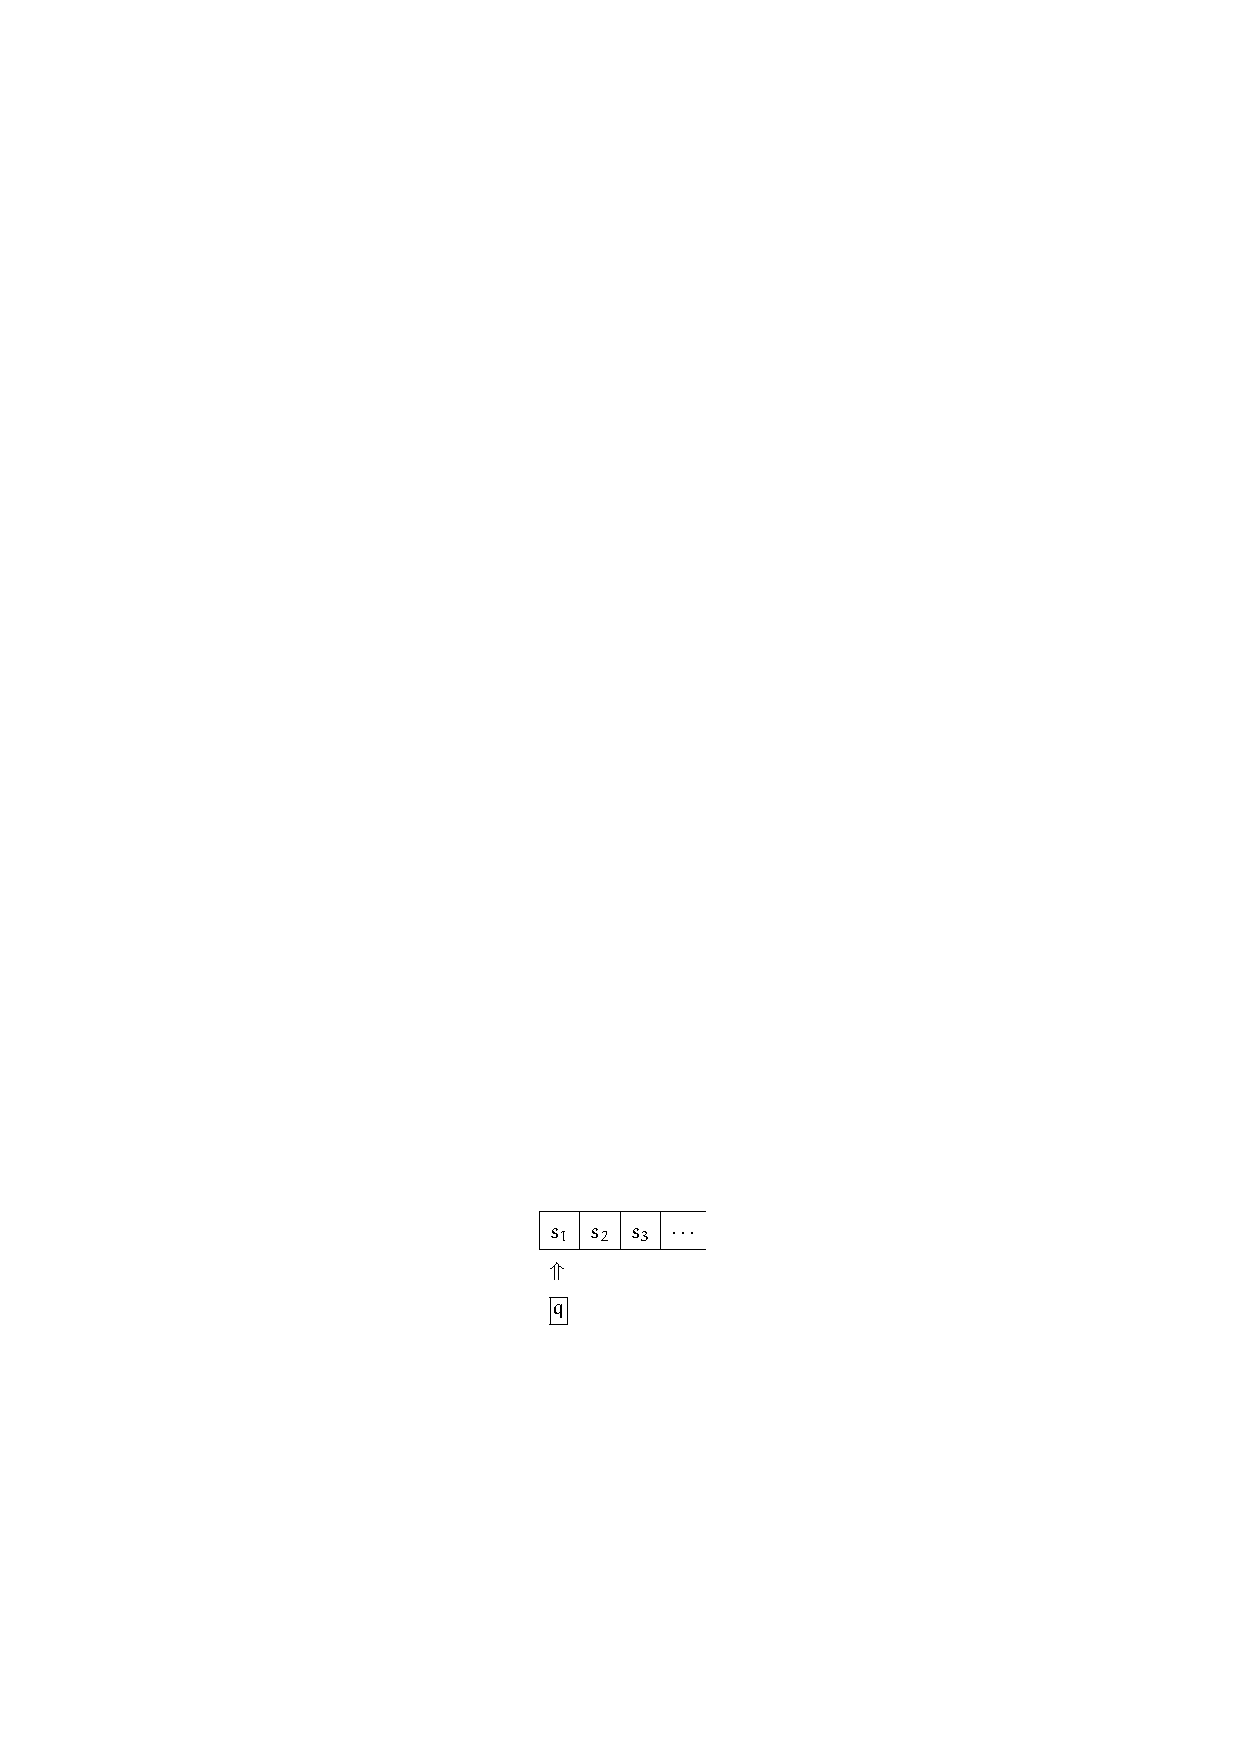
\includegraphics[width=0.3\textwidth]{img/automa_generale.pdf}
		\caption{Dispositivo che rappresenta un esempio generalistico di un automa a stati finiti.}
	\end{figure}

	Una volta terminata la lettura, l'automa è in grado di fornire il risultato di accettazione o di refutazione della stringa (parola) letta. Il \textbf{comportamento} dell'automa si \textbf{definisce} in maniera univoca mediante una tabella, chiamata \textbf{matrice di transizione}, come ad esempio:
	
	\begin{table}[!htbp]
		\centering
		
		\begin{tabular}{@{} c c c @{}}
			\toprule
			 & $a$ & $b$ \\
			\midrule
			$q_{0}$ & $q_{1}$ & $q_{2}$ \\
			$q_{1}$ & $q_{1}$ & $q_{0}$ \\
			$q_{2}$ & $q_{1}$ & $q_{0}$ \\
			\bottomrule
		\end{tabular}
		
		\caption{Matrice di transizione.}
		\label{matrice_di_transizione}
	\end{table}

	\newpage

	\noindent
	Tuttavia, la \underline{rappresentazione più comune e chiara} è il \textbf{grafo}:
	
	\begin{itemize}
		\item Gli \textbf{archi} rappresentano le \emph{transizioni} etichettate con il simbolo in lettura;
		\item Lo \textbf{stato iniziale} è rappresentato con la \emph{freccia ``start''};
		\item Gli \textbf{stati finali} sono cerchiati due volte.
	\end{itemize}

	\begin{figure}[!htp]
		\centering
		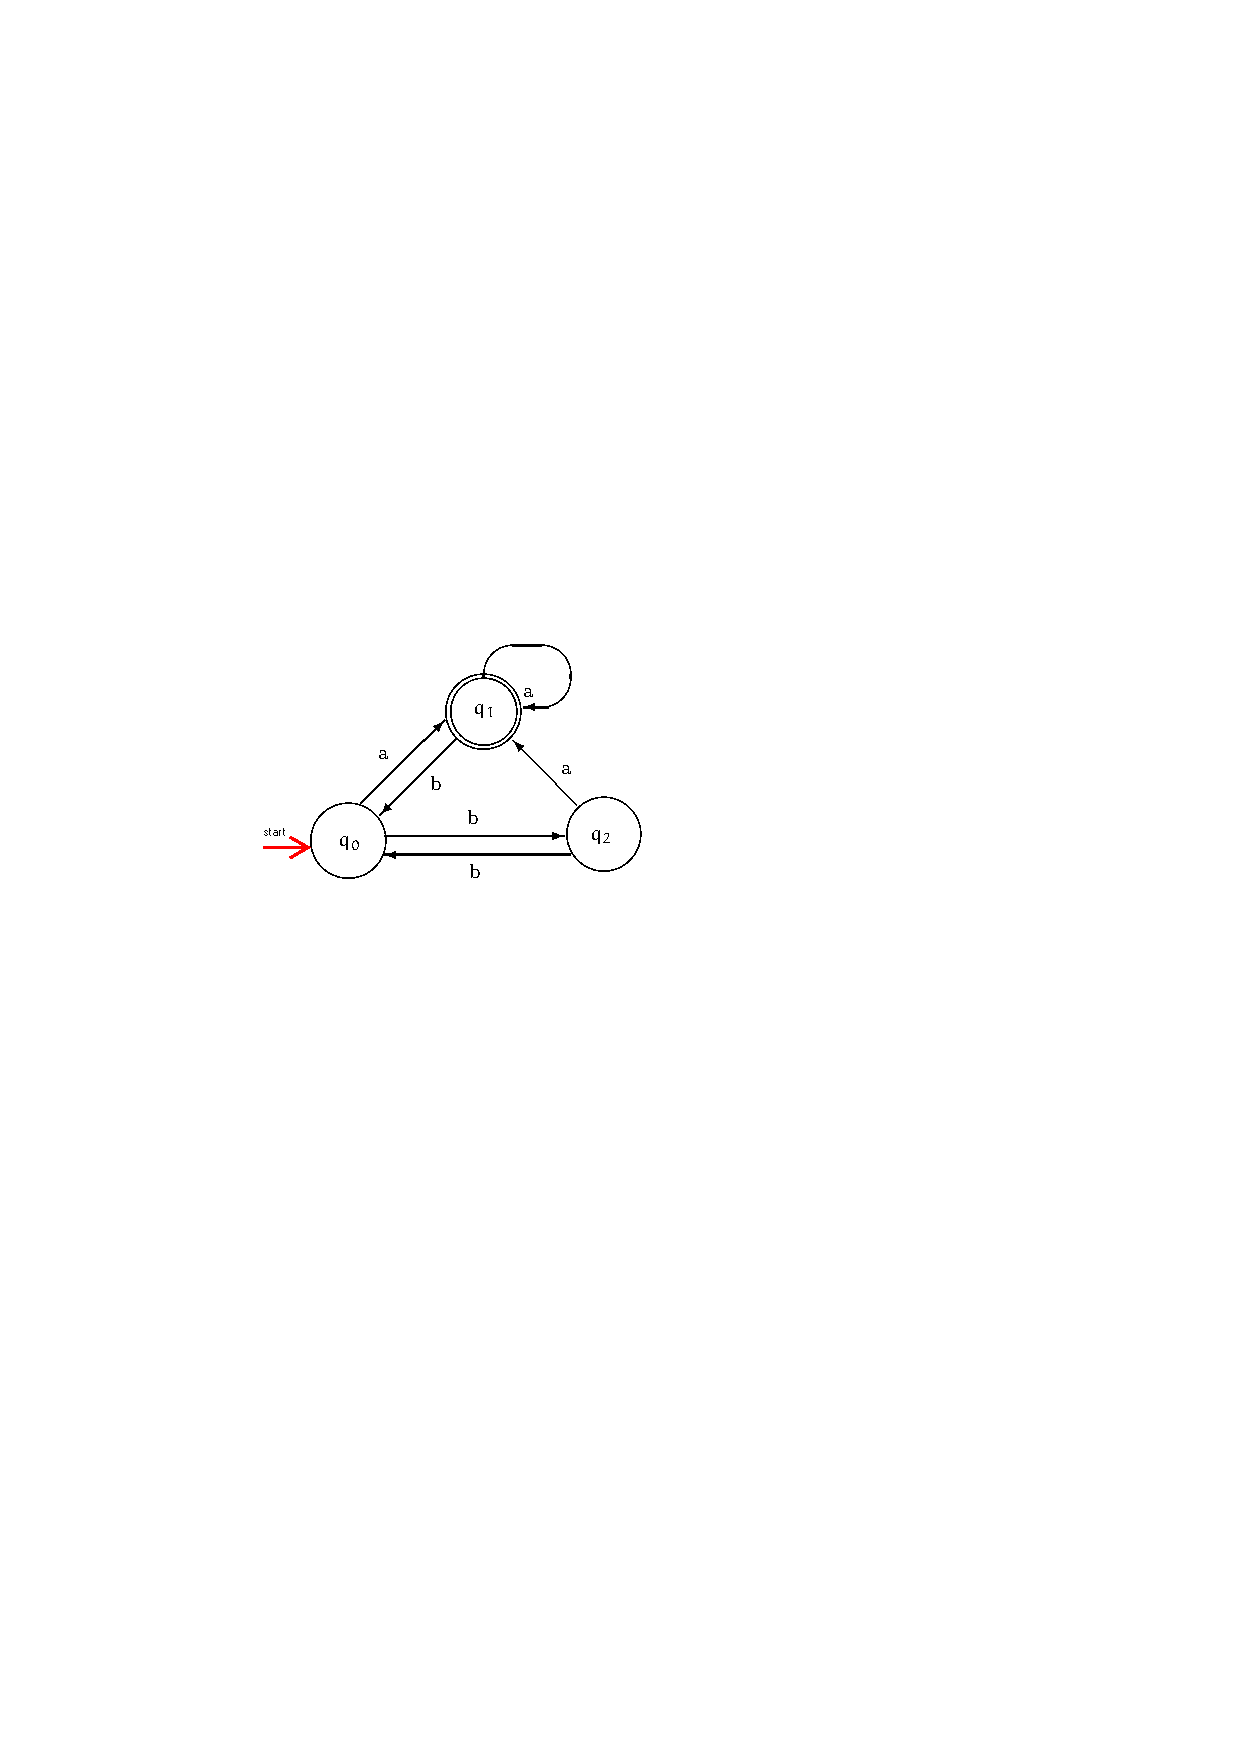
\includegraphics[width=0.5\textwidth]{img/grafo_eg.pdf}
		\caption{Esempio di grafo (freccia start mancante).}
	\end{figure}

	Un \textcolor{Red3}{\textbf{linguaggio vuoto}} è il più piccolo dei linguaggi, si rappresenta con il simbolo $\emptyset$ e si riconosce poiché \textbf{non ha stati finiti} (quindi nessun nodo con il doppio cerchio). Infine, il \textcolor{Red3}{\textbf{linguaggio più grande}} è il linguaggio più grande, si rappresenta con il simbolo $\Sigma^{*}$, esiste dunque la relazione $\emptyset \subseteq \Sigma^{*}$ e si riconosce perché \textbf{ha \underline{solo} stati finiti} (quindi nessun nodo con un solo cerchio).

	\newpage

	\subsubsection{Automi deterministici (DFA)}\label{automi deterministici}
	
	Un \textbf{automa a stati finiti \underline{deterministico}} (DFA) è una che, date determinate condizioni, è possibile determinare la serie di operazioni. Viene rappresentato con una quintupla del tipo $\left\langle Q, \Sigma, \delta, q_0, F\right\rangle$ in cui:
	
	\begin{itemize}
		\item[\ding{42}] $Q$ è un insieme di \textcolor{Red3}{\textbf{stati finiti}};
		
		\item[\ding{42}] $\Sigma$ è un \textcolor{Red3}{\textbf{alfabeto finito}}, cioè un alfabeto di input;
		
		\item[\ding{42}] $\delta: Q \times \Sigma \longrightarrow Q$ è la \textcolor{Red3}{\textbf{funzione di transizione}} che dato lo stato $q \in Q$ in cui si trova la macchina ed un simbolo $a \in \Sigma$ in lettura del nastro, produce il prossimo stato $\delta (q,a) \in Q$ in cui si troverà la macchina;
		
		\item[\ding{42}] $q_0$ è lo \textcolor{Red3}{\textbf{stato iniziale}};
		
		\item[\ding{42}] $F \subseteq Q$ è l'insieme degli \textcolor{Red3}{\textbf{stati finali}}, anche detti \textbf{di accettazione}.
		
		\item[\ding{42}] $\overset{\wedge}{\delta}: Q \times \Sigma^{*} \longrightarrow Q$ si ottiene dalla funzione $\delta$ ed è definita nel seguente modo:
		
		\begin{equation*}
			\begin{cases}
				\overset{\wedge}{\delta}(q, \varepsilon) = q \\
				\overset{\wedge}{\delta}(q, wa) = \delta \left(\overset{\wedge}{\delta}(q, w), a\right)
			\end{cases}
		\end{equation*}
	\end{itemize}

	Sia $M = \left\langle Q, \Sigma, \delta, q_0, F\right\rangle$ un automa a stati finiti \underline{deterministico}. Una \textbf{stringa} $x$ è detta \textbf{accettata} da un $M$ se $\overset{\wedge}{\delta}(q_{0}, x) \in F$. Inoltre, il \textbf{linguaggio è accettato dalla macchina} $M$, denotato come $L(M)$, è l'insieme di tutte le stringhe accettate da $M$, ovvero:
	
	\begin{equation*}
		L(M) = \left\{x \in \Sigma^{*} \: | \: \overset{\wedge}{\delta}(q_0, x) \in F\right\}
	\end{equation*}

	\noindent
	\textbf{N.B. A lezione al posto di $w$ e $x$ è stato utilizzato $\sigma.$}\newline
	
	\noindent
	Un linguaggio $L$ viene detto \textcolor{Red3}{\textbf{\emph{linguaggio regolare}}} se è accettato da qualche automa a stati finiti deterministico (DFA), ovvero se esiste $M$ tale che $L = L(M)$.
	
	\newpage
	
	\subsubsection{Esempio esercizio (automi deterministici)}
	
	\textcolor{Red3}{\textbf{\emph{Esercizio.}}}
	
	\noindent
	Il grafo dell'esercizio è il seguente:
	
	\begin{figure}[!htp]
		\centering
		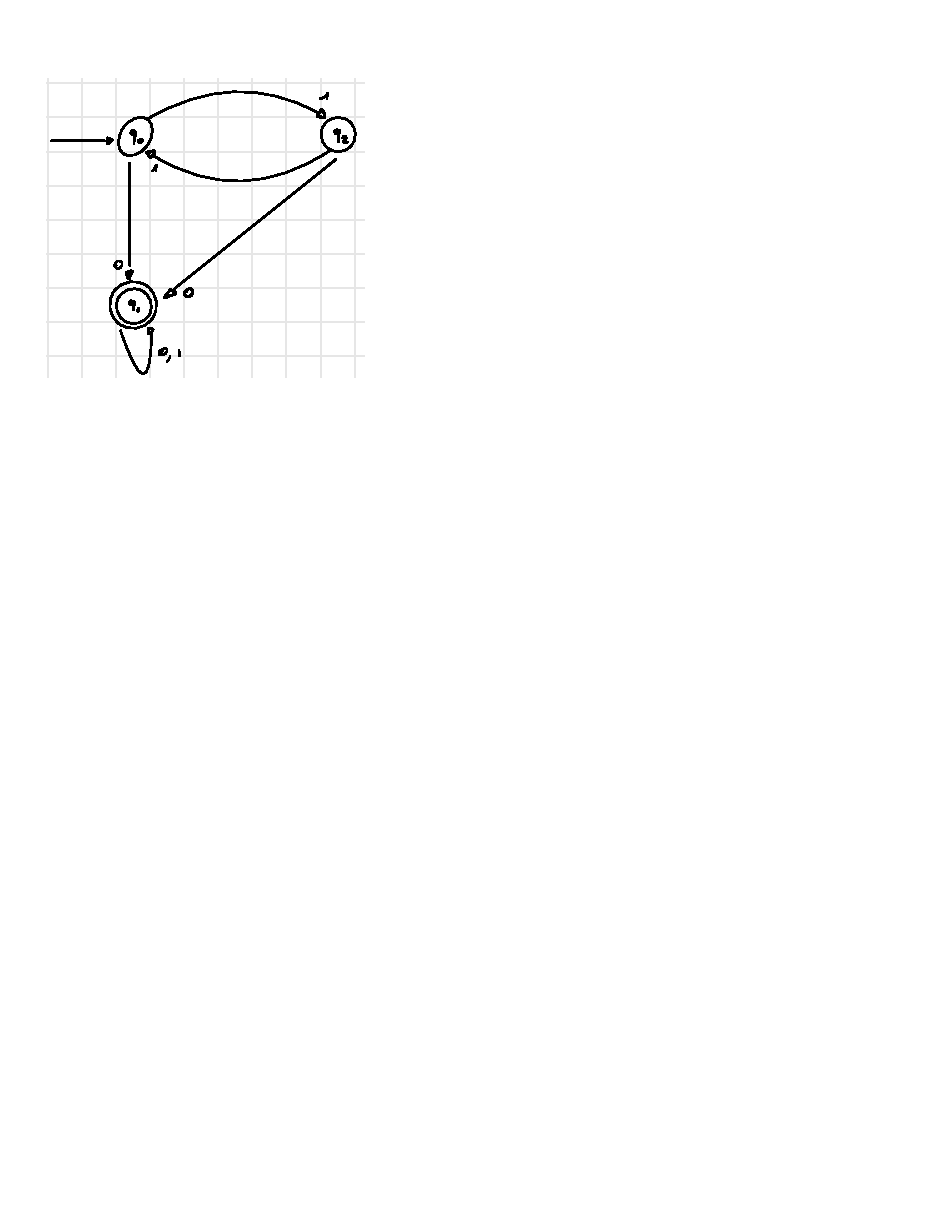
\includegraphics[width=0.6\textwidth]{img/grafo_ex1.pdf}
		\caption{Grafo di un automa a stati finiti deterministico.}
	\end{figure}
	
	\noindent
	I dati forniti sono i seguenti:
	
	\begin{gather*}
		\textbf{Linguaggio: } L(M) = \left\{x \in \{0, 1\}^* \: | \: x \text{ contiene almeno uno } 0 \right\} \\
		\textbf{Alfabeto: } \Sigma = \left\{0, 1\right\}
	\end{gather*}
	
	\noindent
	Si dimostri che $L(M)$ è $\subseteq$ e $\supseteq$ del linguaggio che è stato dato. Quindi, è necessario verificare le condizioni con:
	
	\begin{equation*}
		\left\{x \in \{0, 1\}^* \: | \: x \text{ contiene almeno uno } 0 \right\}
	\end{equation*}
	\newline
	\noindent
	\textcolor{Green4}{\textbf{\emph{Risoluzione.}}}
	
	\noindent
	La stringa $x$ è sicuramente formata da:
	
	\begin{equation*}
		x = 1^{n}\: 0 \: w \in \{0,1\}^{*} \text{ e } n \in \mathbb{N}
	\end{equation*}
	
	\noindent
	In cui ci deve essere un numero $n$ di concatenazioni di numeri $1$, uno $0$ come viene specificato \dquotes{$x \text{ contiene almeno uno } 0$} e infine una qualsiasi stringa dell'alfabeto $w$. L'\textbf{obbiettivo} è dimostrare che:
	
	\begin{equation*}
		\forall w \in \left\{0, 1\right\}^{*} : \overset{\wedge}{\delta} (q_{1}, w) = q_{1}
	\end{equation*}

	\noindent
	Ovvero che dato qualsiasi simbolo appartenente all'alfabeto, lo stato successivo sia sempre $q_{1}$, ovvero quello finale!
	
	\newpage
	
	Si supponga che la cardinalità di $w$, ovvero la lunghezza della stringa, sia uguale a $m$, cioè $|w| = m$. Questo implica che lo stato non varia:
	
	\begin{equation*}
		m = 0 \Longrightarrow w = \varepsilon \hspace{1em} \text{ e quindi } \hspace{1em} \overset{\wedge}{\delta} (q_{1}, w) = q_{1}
	\end{equation*}

	\noindent
	Invece, il caso in cui la stringa non sia vuota:
	
	\begin{equation*}
		m \ge 0 \text { e } m+1 \Longrightarrow w = \sigma 0 \hspace{1em} \textbf{ oppure } \hspace{1em} w = \sigma 1
	\end{equation*}

	\noindent
	Per \textbf{induzione} si riesce a dimostrare che:
	
	\begin{equation*}
		\overset{\wedge}{\delta} \left(q_{1}, \sigma 0\right) = \delta\left(\overset{\wedge}{\delta} \left(q_{1}, \sigma\right), 0\right) = \delta \left(q_{1}, 0\right) = q_{1}
	\end{equation*}
	
	\noindent
	Grazie all'induzione è stato dimostrato che se era vero per $m$, allora è vero anche per $m+1$, quindi qualsiasi $m$ (maggiore o uguale a zero ovviamente). Quindi, il \textbf{primo passo dell'esercizio è stato concluso, ovvero quello di dimostrare che la $w$ è sempre accettata soltanto se posta dopo il primo zero} (sequenza conclusiva dell'automa a stati finiti deterministico).\newline
	
	Adesso si prosegue la dimostrazione dimostrando che per ogni numero naturale, con una sequenza di $1$ si finisce nello stato $q_{0}$ o $q_{2}$, ovvero l'automa non termina.
	
	
	\noindent
	\textbf{\emph{\underline{Caso base}}}:
	
	
	\begin{itemize}
		\item $n = 0: \hspace{1em} \overset{\wedge}{\delta} \left(q_{0}, \varepsilon\right) = q_{0} \in \left\{q_{0}, q_{2}\right\}$
		\item $n \ge 0: \hspace{1em} \overset{\wedge}{\delta} \left(q_{0}, 1^{n+1}\right) = \overset{\wedge}{\delta} \left(q_{0}, 1^{n} \: 1\right) = \delta \left(\overset{\wedge}{\delta} \left(q_{0}, 1^{n}\right)\right) \in \left\{q_{0}, q_{2}\right\}$
	\end{itemize}

	\noindent
	\textcolor{Green4}{\textbf{\checkmark Dimostrato}} che ogni stringa in forma $x \in L$ (ogni stringa nel linguaggio), è accettata dall'automa. Ovvero $L \subseteq L\left(M\right)$.\newline
	
	L'esercizio si conclude con la dimostrazione $L \supseteq L\left(M\right)$- Quindi se $x$ non contiene almeno uno zero ($x = 1^{n}$), allora si può affermare con certezza che $x$ non è in $L\left(M\right) = \left\{\sigma \: | \: \overset{\wedge}{\delta} \left(q_{0}, \sigma\right) = q_{1}\right\}$. Quindi formalmente:
	
	\begin{equation*}
		\forall n : 1^{n} \Longrightarrow \overset{\wedge}{\delta} \left(q_{0}, x\right) \in \left\{q_{0}, q_{2}\right\} \hspace{2em} \textcolor{Green4}{\textbf{\checkmark Dimostrato}}
	\end{equation*}

	\newpage
	
	\subsubsection{Automi non-deterministici (NFA)}\label{automi non-deterministici}
	
	Un \textbf{automa a stati finiti \underline{non-deterministico}} (NFA) è una quintupla $\left\langle Q, \Sigma, \delta, q_0, F\right\rangle$ dove $Q, \Sigma, q_{0}$ e $F \subseteq Q$ mantengono il significato visto per gli automi deterministici (pagina~\pageref{automi deterministici}), mentre la \textbf{funzione di transizione} $\delta$ è definita come:
	
	\begin{equation*}
		\delta : Q \times \Sigma \longrightarrow P(Q) = 2^{Q} = 2^{|Q|}
	\end{equation*}

	\noindent
	Ovvero è una relazione tra stati.

	In particolare, si tratta di un concetto fondamentale in informatica che definisce un \textbf{modello (ideale)} di calcolo parallelo su cui si fonda la moderna analisi della complessità degli algoritmi.
	
	Adesso è possibile avere $\delta \left(q, a\right) = \emptyset$ per qualche $q \in Q$ ed $a \in \Sigma$, poiché l'\textcolor{Red3}{\textbf{automa non può avere transizioni per alcuni simboli in input}}.\newline
	
	\noindent
	Si definisce la funzione $\overset{\wedge}{\delta} : Q \times \Sigma^{*} \longrightarrow P\left(Q\right)$ nel seguente modo:
	
	\begin{equation*}
		\begin{cases}
			\overset{\wedge}{\delta} \left(q, \varepsilon\right) = \left\{q\right\} \\
			\overset{\wedge}{\delta} \left(q, wa\right) = \bigcup_{p \in \overset{\wedge}{\delta} \left(q, w\right)} \delta \left(p, a\right)
		\end{cases}
	\end{equation*}

	\noindent
	Inoltre, si dice che \textcolor{Red3}{\textbf{una \underline{stringa} $x$ è accettata da un automa a stati finiti non-deterministici NFA}} $M = \left\langle Q, \Sigma, \delta, q_{0}, F\right\rangle$ \textbf{se}:
	
	\begin{equation*}
		\overset{\wedge}{\delta} \left(q_{0}, x\right) \cap F \ne \emptyset
	\end{equation*}

	\noindent
	In altre parole, una stringa è accettata quando una di queste computazioni raggiunge uno stato finale dopo aver consumato la sequenza in input.

	Invece, si dice che \textcolor{Red3}{\textbf{un \underline{linguaggio} è accettato da un automa a stati finiti non-deterministici NFA}} $M$ \textbf{se corrisponde all'insieme delle stringhe accettate}:
	
	\begin{equation*}
		L\left(M\right) = \left\{x \in \Sigma^{*} \: \left| \: \hat{\delta} \left(q_{0}, x\right) \cap F \ne \emptyset\right.\right\}
	\end{equation*}

	La rappresentazione a grafo rimane pressoché immutata. L'\textbf{unica differenza} è che da un nodo possono uscire più archi (o nessuno) etichettati dallo stesso simbolo.
	
	\newpage
	
	\subsubsection{Teorema Rabin-Scott (1959)}
	
	\begin{theorem}[\textbf{Rabin-Scott}] \label{rabin-scott}
		Sia $M = \left\langle Q, \Sigma, \delta, q_{0}, F \right\rangle$ un automa a stati finiti non deterministica (NFA). Allora esiste un automa a stati finiti deterministica $M^{'}$ tale che $L\left(M\right) = L(M^{'})$.
	\end{theorem}

	\begin{proof}[\textbf{Dimostrazione}]
		Si definisce l'automa a stati finiti non deterministica con la quintupla $M^{'} = \left\langle\ Q^{'}, \Sigma^{'}, \delta^{'}, q_{0}^{'}, F^{'} \right\rangle$ e con le seguenti proprietà:
		
		\begin{itemize}
			\item[\ding{72}] $\Sigma^{'} = \Sigma$.
			
			\item[\ding{72}] $Q^{'} = P(Q)$, sarebbe più preciso definire $Q^{'} = \left\{q_{1}, \cdots, q_{2\: |Q|}\right\}$ e poi stabilire una corrispondenza biunivoca fra tali stati e gli elementi di $P(Q)$. Tuttavia, così facendo rimane più chiara la dimostrazione.
			
			\item[\ding{72}] $q_{0}^{'} = \left\{q_{0}\right\}$.
			
			\item[\ding{72}] $F^{'} = \left\{P \subseteq Q \: | \: P \cap F \ne \emptyset\right\}$
			
			\item[\ding{72}] $\delta^{'}\left(\mathrm{P}, a\right) = \bigcup_{p \in \mathrm{P}} \delta \left(p, a\right)$, per ogni $\mathrm{P} \in P(Q)$
		\end{itemize}
	
		Si mostra, \textbf{per induzione}, sulla lunghezza della stringa di input $\sigma \in \Sigma^{*}$ che:
		
		\begin{equation}\label{induzione rabin-scott}
			\forall \sigma \in \Sigma^{*} : \overset{\wedge}{\delta} \left(q_{0}, x\right) = \overset{\wedge}{\delta^{'}} \left(q_{0}^{'}, x\right)
		\end{equation}
	
		\noindent
		In cui la parte di sinistra è per gli automi non deterministici ($\overset{\wedge}{\delta} \left(q_{0}, x\right)$), mentre la parte di destra è per gli automi deterministici $\left(\overset{\wedge}{\delta^{'}} \left(q_{0}^{'}, x\right)\right)$.\newline
		
		\noindent
		\textbf{\emph{\underline{Caso base.}}}\footnote{Il simbolo $\iff$ indica \dquotes{se e solo se}.}
		
		\begin{equation*}
			|\sigma| = 0 \iff \sigma = \varepsilon : \overset{\wedge}{\delta} \left(q_{0}, \varepsilon\right) = \left\{q_{0}\right\} = q^{'}_{0} = \overset{\wedge}{\delta^{'}} \left(q_{0}^{'}, \varepsilon\right)
		\end{equation*}
	
		\noindent
		\textbf{\emph{\underline{Passo induttivo.}}}
		
		\begin{equation*}
			\forall \sigma \in \Sigma^{*} : |\sigma| \le n : \overset{\wedge}{\delta} \left(q_{0}, \sigma\right) = \overset{\wedge}{\delta} \left(q_{0}, \sigma\right)
		\end{equation*}
	
		\noindent
		Quindi che non ci siano gli apici $'$ come nell'equazione~\ref{induzione rabin-scott}. Si dimostra induttivamente:
		
		\begin{equation*}
			\overset{\wedge}{\delta^{'}} \left(q_{0}^{'}, \sigma a\right) = \delta^{'} \left(\overset{\wedge}{\delta^{'}}\left(q_{0}^{'}, a\right), a\right) = \delta^{'} \left(\overset{\wedge}{\delta}\left(q_{0}, \sigma\right), a\right) = \bigcup_{p \in \overset{\wedge}{\delta}\left(q_{0}, \sigma\right)} \delta\left(p, a\right) = \overset{\wedge}{\delta} \left(q_{0}, \sigma a\right)
		\end{equation*}
	
		\noindent
		In cui $p \in \overset{\wedge}{\delta}\left(q_{0}, \sigma\right)$ e $\overset{\wedge}{\delta} \left(q_{0}, \sigma a\right)$ sono \textbf{macchine deterministiche}.
		
		\noindent
		La dimostrazione si conclude con le seguenti ovvie relazioni:
		
		\begin{gather*}
			\sigma \in L \iff
			\overset{\wedge}{\delta}\left(q_{0}, \sigma\right) \cap F \ne 0 \iff
			\overset{\wedge}{\delta^{'}}\left(q_{0}^{'}, \sigma\right) \cap F \ne \emptyset \iff
			\overset{\wedge}{\delta^{'}}\left(q_{0}^{'}, \sigma\right) \in F^{'} \iff
			\sigma \in L\left(M^{'}\right)
		\end{gather*}
	\end{proof}
	
	\newpage
	
	\subsubsection{Esempio esercizio (automi non-deterministici)}
	
	\textcolor{Red3}{\textbf{\emph{Esercizio.}}}
	
	\noindent
	Il grafo dell'esercizio è il seguente:
	
	\begin{figure}[!htp]
		\centering
		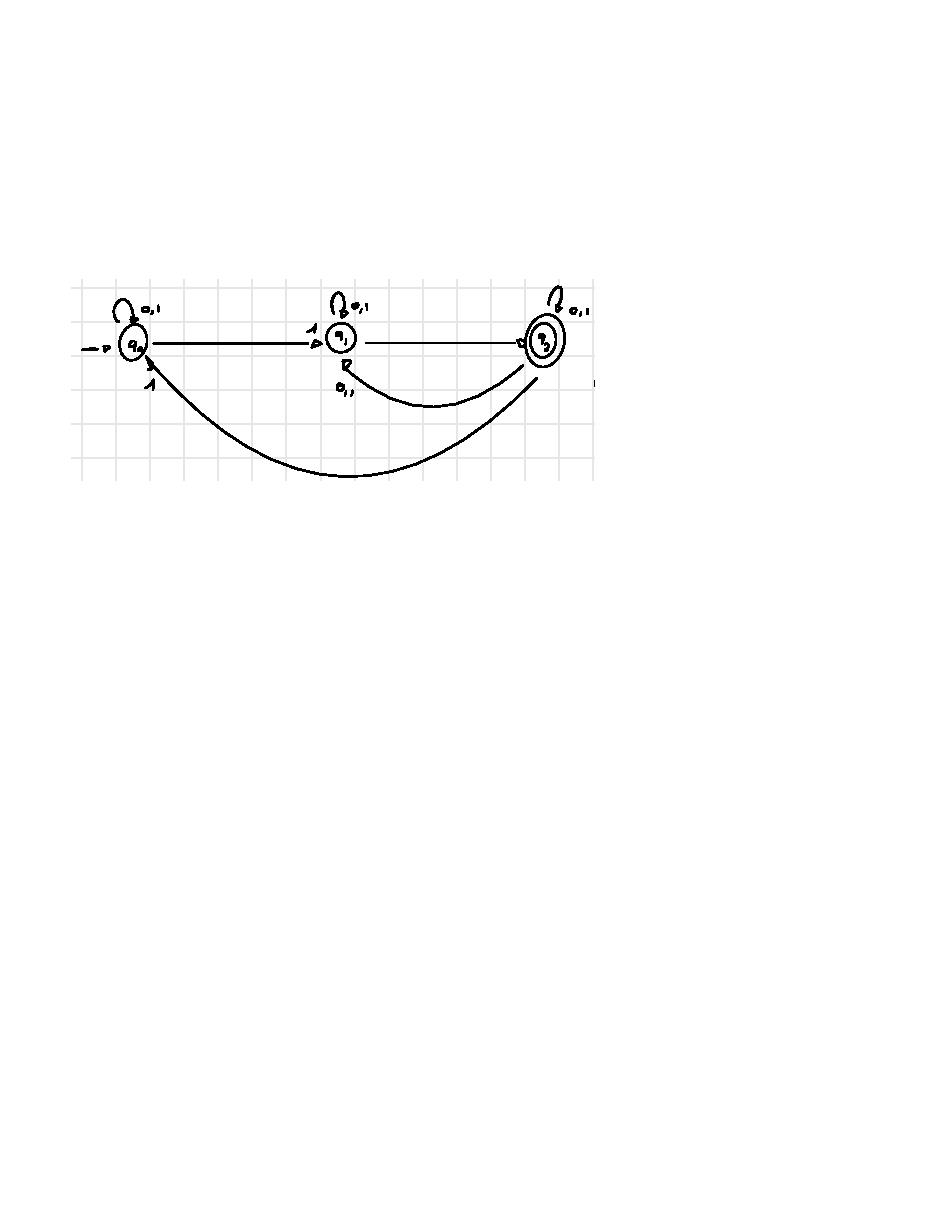
\includegraphics[width=0.7\textwidth]{img/grafo_ex2.pdf}
		\caption{Grafo di un automa a stati finiti non-deterministico.}
	\end{figure}
	
	\noindent
	\textcolor{Green4}{\textbf{\emph{Risoluzione.}}}
	
	\noindent
	La $Q$ è formata da $\left\{q_{0}, q_{1}, q_{2}\right\}$, mentre la $P(a)$ ha i seguenti insiemi:
	
	\begin{equation*}
		P\left(a\right) = \left\{
		\emptyset, \left\{q_{0}\right\},
		\left\{q_{1}\right\},
		\textcolor{Red3}{\left\{q_{2}\right\}}, \left\{q_{0}, q_{1}\right\},
		\textcolor{Red3}{\left\{q_{0}, q_{2}\right\}, \left\{q_{1}, q_{2}\right\},
		\left\{q_{0}, q_{1}, q_{2}\right\}}\right\}
	\end{equation*}

	\noindent
	Le espressioni in rosso sono sequenze finite che terminano.
	
	\noindent
	Infine, l'automa non-deterministico è riconducibile a un automa deterministico:
	
	\begin{equation*}
		\delta^{'} \left(s, a\right) = \bigcup_{q \in S} \delta \left(q, a\right)
	\end{equation*}

	\begin{figure}[!htp]
		\centering
		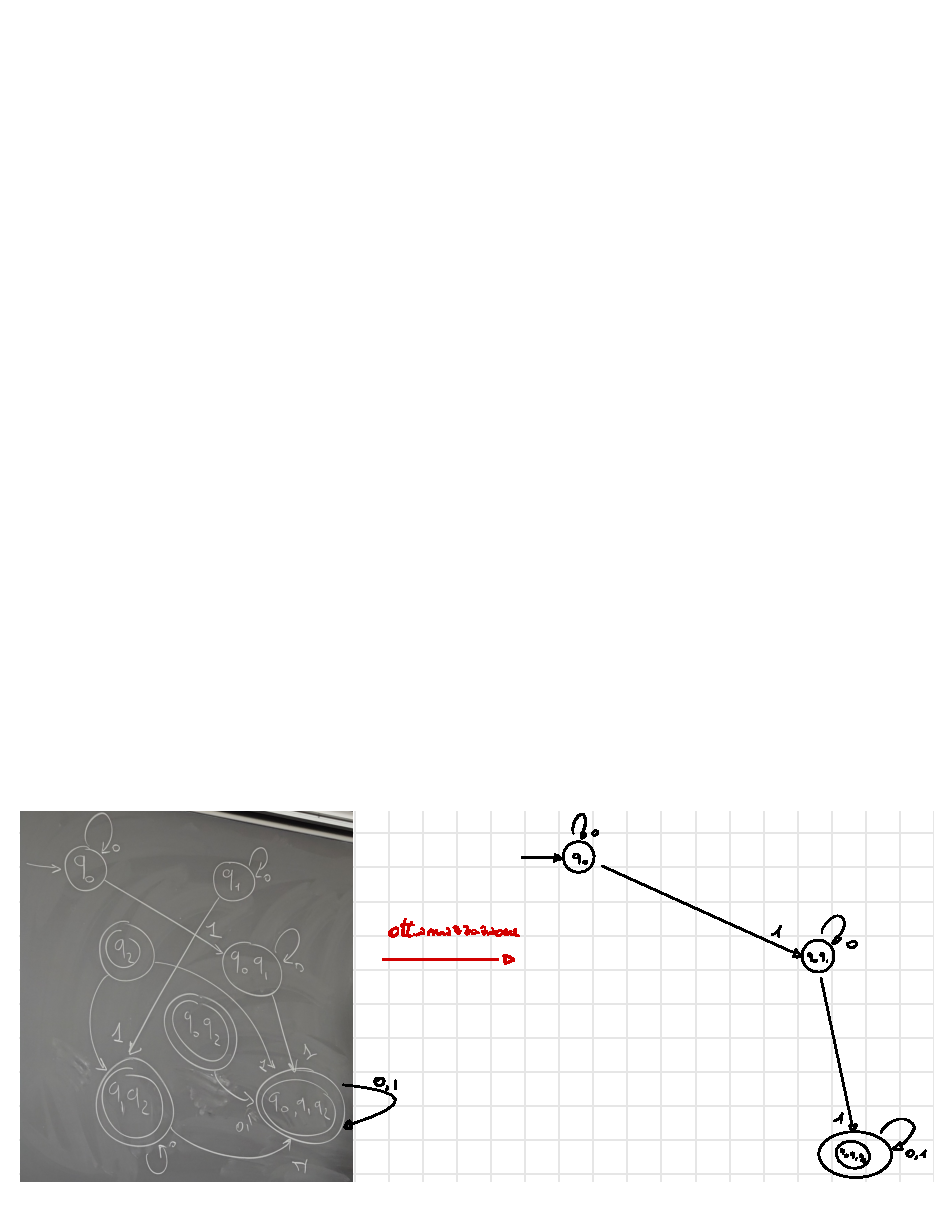
\includegraphics[width=1\textwidth]{img/grafo_ex2-sol.pdf}
		\caption{Rappresentazione di una conversione da non-deterministico a deterministico con relativa ottimizzazione.}
	\end{figure}

	\newpage
	
	\subsubsection[\textcolor{Red3}{Esercizi da esame}]{Esercizi da esame}\label{Esercizi da esame - ASFD / linguaggi regolari}
	
	\textcolor{Red3}{\textbf{\underline{Esercizio 1}}}\newline
	
	\noindent
	I dati dell'esercizio sono i seguenti:
	
	\begin{gather*}
		L = \left\{x \hspace{0.5em} | \hspace{0.5em} |x_{0}| = 2\mathbb{N}\right\} \\
		\Sigma = \left\{0, 1\right\}
	\end{gather*}\newline
	
	\noindent
	\textcolor{Green4}{\textbf{\emph{Risoluzione.}}}\newline
	
	\noindent
	L'automa da costruire si basa sulla condizione del linguaggio, ovvero che $x_{0}$ (\textbf{numero degli zeri di $x$}) sia uguale a $2\mathbb{N}$ (\textbf{numero pari}).\footnote{Un numero dispari si rappresenta come $2\mathbb{N} + 1$.}
	
	\begin{figure}[!htp]
		\centering
		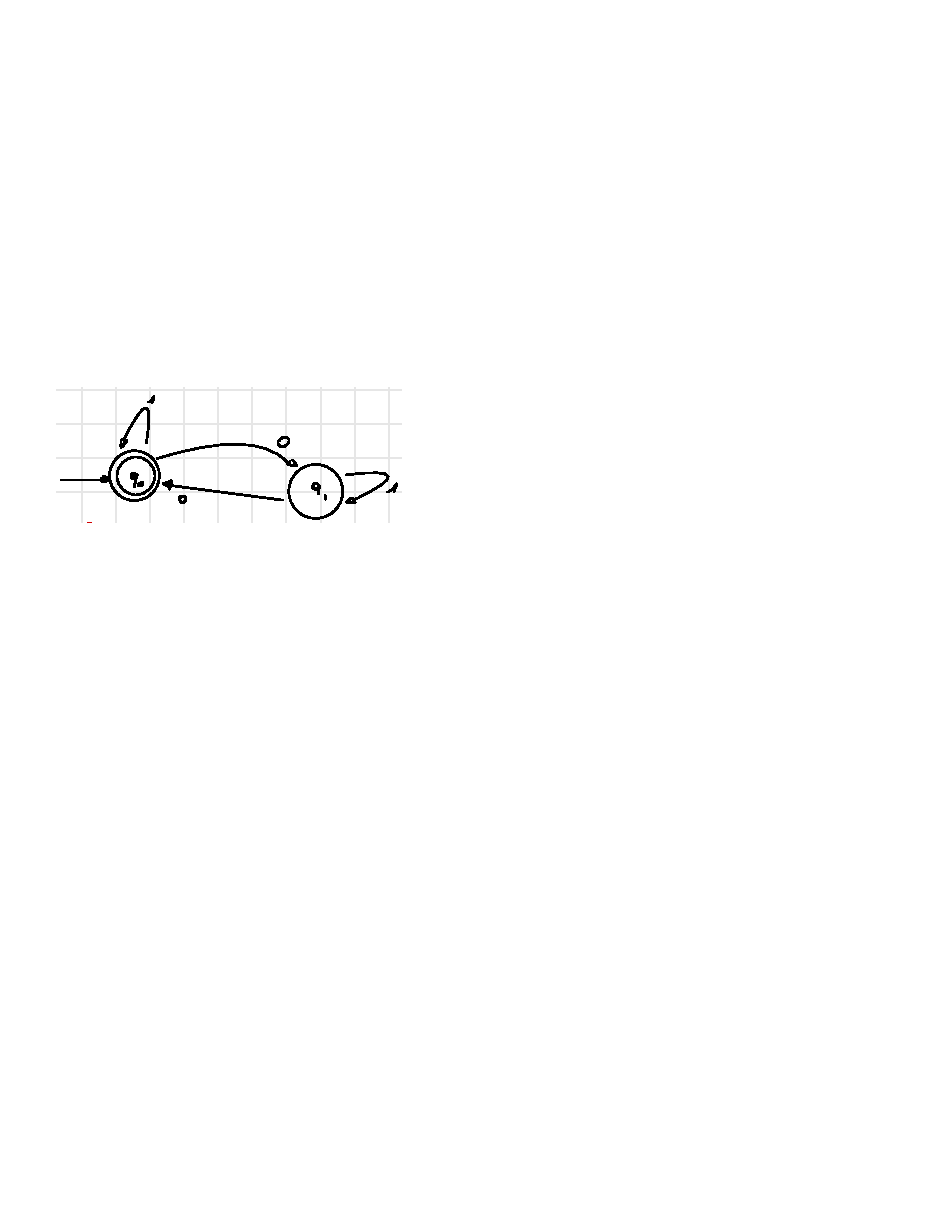
\includegraphics[width=0.8\textwidth]{img/esercitazioni/01_exe1.pdf}
		\caption{Grafo dell'automa a stati finiti deterministico dell'esercizio 1.}\label{ASFD-esercizio_1}
	\end{figure}

	\noindent
	L'\textbf{unica osservazione} da effettuare è che lo stato $q_{0}$ è finito poiché la macchina deve terminare sia per un numero pari di zeri, ma anche nel caso in cui venga si presenti una stringa vuota poiché zero $0$ è pari.

	\newpage

	\begin{proof}[\textcolor{Blue3}{\textbf{Dimostrazione}}]
		Si vuole dimostrare inizialmente che $\sigma \in L \iff \delta\left(q_{0}, \sigma\right) \in F$ tramite l'induzione.\newline
		
		\noindent
		\textbf{\underline{Caso base.}}
		
		\begin{enumerate}
			\item $x = \varepsilon \in L \longrightarrow \delta\left(q_{0}, \varepsilon\right) = q_{0} \in F$
			\item $x = 0 \notin L \longrightarrow \delta\left(q_{0}, 0\right) = q_{1} \notin F$
		\end{enumerate}
	
		\noindent
		In altre parole, se la stringa in entrata è vuota, cioè $\varepsilon$, allora l'automa rimane in $q_{0}$, cioè lo stato finito e quindi appartiene al linguaggio e all'insieme $F$. Nel caso in cui la stringa \underline{non} è vuota, dallo stato $q_{0}$ si finisce in $q_{1}$, il quale non appartiene né al linguaggio né all'insieme $F$ dato che non l'automa non finisce in uno stato di fine.\newline
		
		\noindent
		\textbf{\underline{Ipotesi induttiva.}}\newline
		
		\noindent
		Per $x$ con $|x| < n$, cioè con la lunghezza della stringa $x$ minore di $n$, allora $x \in L \Longrightarrow \delta\left(q_{0}, x\right) \in F$.
		
		\noindent
		Allora si ipotizzi una $x$ di lunghezza $n + 1$ che dunque non appartiene né al linguaggio:
		
		\begin{equation*}
			x^{'} = x 0 \notin L
		\end{equation*}
	
		\noindent
		Né all'insieme $F$:
		
		\begin{equation*}
			\delta\left(q_{0}, x^{'}\right) = \delta\left(q_{0}, x0\right) = \delta\left(q_{0}, 0\right) = q_{1} \notin F
		\end{equation*}
	
		\noindent
		Dallo stato $q_{0}$ con una stringa $x$ si rimane in $q_{0}$ (formalmente $\delta\left(q_{0}, x\right) = q_{0}$).
		
		\noindent
		È stato inserito uno $0$ nella dimostrazione, ma era possibile dimostrarlo anche tramite $1$, cioè:
		
		\begin{equation*}
			x^{'} = x 1 \notin L
		\end{equation*}
	
		\noindent
		Né all'insieme $F$:
		
		\begin{equation*}
			\delta\left(q_{0}, x^{'}\right) = \delta\left(q_{0}, x1\right) = \delta\left(q_{0}, 1\right) = q_{0} \in F
		\end{equation*}
	\end{proof}

	\newpage

	\begin{proof}[\textcolor{Blue3}{\textbf{Dimostrazione 2}}]
		Questa seconda dimostrazione ha l'obbiettivo di dimostrare, pardon per il gioco di parole, l'espressione $\sigma \notin L \Longrightarrow \delta\left(q_{0}, \sigma\right) \notin F$ tramite l'induzione. La differenza dalla dimostrazione precedente sta nel dimostrare la \textbf{\emph{non appartenenza}} al linguaggio e all'insieme degli stati finiti $F$.\newline
		
		\noindent
		\textbf{\underline{Caso base.}}\newline
		
		\noindent
		Si utilizza quello della dimostrazione precedente, quindi:
		
		\begin{enumerate}
			\item $x = \varepsilon \in L \longrightarrow \delta\left(q_{0}, \varepsilon\right) = q_{0} \in F$
			\item $x = 0 \notin L \longrightarrow \delta\left(q_{0}, 0\right) = q_{1} \notin F$
		\end{enumerate}
	
		\noindent
		\textbf{\underline{Ipotesi induttiva.}}\newline
		
		\noindent
		Per $x$ con $|x| < n$, cioè con la lunghezza della stringa $x$ minore di $n$, allora $x \notin L \Longrightarrow \delta\left(q_{0}, x\right) \notin F$.
		
		\noindent
		In questa dimostrazione si considerano le stesse casistiche precedenti, quindi con $0$ e $1$:
		
		\begin{gather*}
			x^{'} = x 0 \in L \longrightarrow \delta\left(q_{0}, x^{'}\right) = \delta\left(q_{0}, x_{0}\right) = \delta\left(q_{1}, 0\right) = q_{0} \in F \\
			x^{'} = x 1 \in L \longrightarrow \delta\left(q_{0}, x^{'}\right) = \delta\left(q_{0}, x_{1}\right) = \delta\left(q_{1}, 1\right) = q_{1} \notin F
		\end{gather*}
	\end{proof}

	\newpage
	
	\noindent
	\textcolor{Red3}{\textbf{\underline{Esercizio 2}}}\newline
	
	\noindent
	I dati dell'esercizio sono i seguenti:
	
	\begin{gather*}
		L = \left\{x \hspace{0.5em} | \hspace{0.5em} |x_{0}| = 1\right\} \\
		\Sigma = \left\{0, 1\right\}
	\end{gather*}\newline

	\noindent
	\textcolor{Green4}{\textbf{\emph{Risoluzione.}}}\newline
	
	\noindent
	L'automa da costruire si basa sulla condizione del linguaggio, ovvero che $x_{0}$ (\textbf{numero degli zeri di $x$}) sia uguale a $1$.
	
	\begin{figure}[!htp]
		\centering
		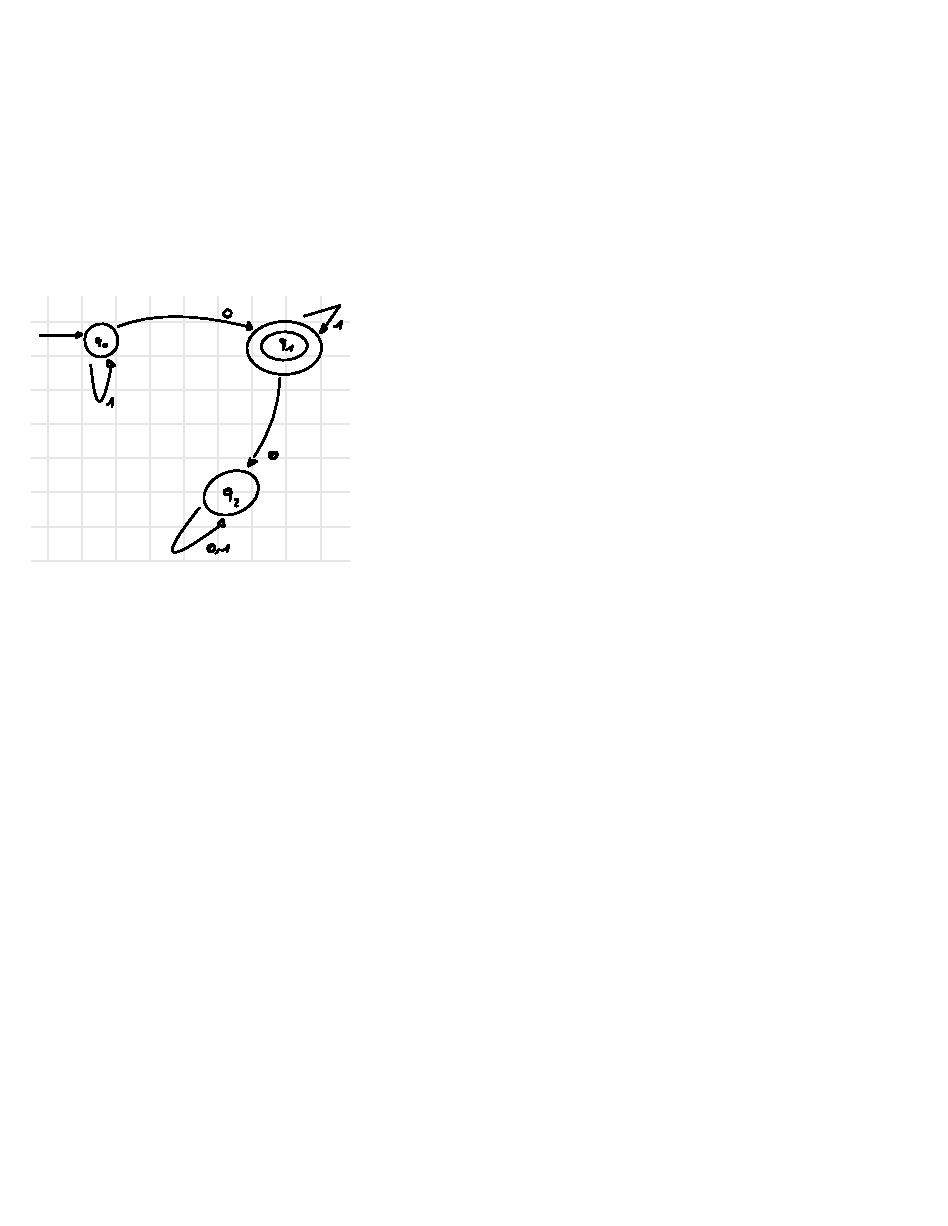
\includegraphics[width=0.8\textwidth]{img/esercitazioni/01_exe2.pdf}
		\caption{Grafo dell'automa a stati finiti deterministico dell'esercizio 2.}\label{ASFD-esercizio_2}
	\end{figure}
	
	\noindent
	Sono \textbf{due} le \textbf{osservazioni} da fare: 
	
	\begin{enumerate}
		\item Dato che è necessario solo uno zero per terminare, lo stato $q_{1}$ è obbligatoriamente uno stato finito;
		\item Lo stato $q_{2}$ esiste solamente per bloccare la macchina nel caso in cui la sequenza sia errata, ovvero nel momento in cui vengano inseriti più zeri. Questo stato particolare prende il nome di \dquotes{\textbf{\underline{stato pozzo}}}.
	\end{enumerate}

	\newpage
	
	\begin{proof}[\textcolor{Blue3}{\textbf{Dimostrazione}}]
		Si vuole dimostrare che $\sigma \in L \iff \delta\left(q_{0}, \sigma\right) \in F$ tramite l'induzione.\newline
		
		\noindent
		\textbf{\underline{Caso base.}}
		
		\begin{enumerate}
			\item $x = \varepsilon \notin L \longrightarrow \delta\left(q_{0}, \varepsilon\right) = q_{0} \notin F$
			\item $x = 0 \in L \longrightarrow \delta\left(q_{0}, 0\right) = q_{1} \in F$
			\item $x = 00 \notin L \longrightarrow \delta(\underbrace{q_{0}, 0}_{q_{1}} 0) = \delta\left(q_{1}, 0\right) = q_{2} \notin F$
		\end{enumerate}
		
		\noindent
		Con il caso base sono stati ricoperti tutti gli stati.\newline
		
		\noindent
		\textbf{\underline{Ipotesi induttiva.}}\newline
		
		\noindent
		Si vuole dimostrare che $\sigma \in L \Longrightarrow \delta\left(q_{0}, \sigma\right) \in F$, allora l'ipotesi induttiva è: se $|x| < n$ allora $x \in L \Longrightarrow \delta\left(q_{0}, x\right) \in F$. Per farlo, si dimostrano le due casistiche classiche:
		
		\begin{itemize}
			\item $x^{'} = x0 \notin L \longrightarrow \delta(\overbrace{q_{0}, x}^{q_{1}} 0) = \delta\left(q_{1}, 0\right) = q_{2} \notin F$
			
			\item $x^{'} = x1 \in L \longrightarrow \delta(\underbrace{q_{0}, x}_{q_{1}} 1) = \delta\left(q_{1}, 1\right) = q_{1} \in F$
		\end{itemize}
	\end{proof}

	\newpage

	\begin{proof}[\textcolor{Blue3}{\textbf{Dimostrazione 2}}]
		Dopo la prima dimostrazione, adesso si vuole dimostrare che $\sigma \notin L \Longrightarrow \delta\left(q_{0}, \sigma\right) \notin F$ tramite l'induzione.\newline
		
		\noindent
		Come caso base si utilizza quello visto nella precedente dimostrazione.\newline
		
		\noindent
		\textbf{\underline{Ipotesi induttiva.}}\newline
		
		\noindent
		Si vuole dimostrare che $\sigma \notin L \Longrightarrow \delta\left(q_{0}, \sigma\right) \notin F$, allora l'ipotesi induttiva è: se $|x| < n$ allora $x \notin L \Longrightarrow \delta\left(q_{0}, x\right) \notin F$. Per farlo, si devono trovare delle casistiche particolari:
		
		\begin{enumerate}[label=\alph*.]
			\item $x = 1^{n}$
			
			\item $x = 1^{n} 0 1^{n} 0 \left\{0, 1\right\}^{n}$
		\end{enumerate}
	
		\noindent
		Le casistiche \dquotes{generali} in cui una stringa non appartiene al linguaggio, e quindi all'insieme degli stati finali $F$, è quando la stringa è formata da una concatenazione di $1$ (caso a), oppure quando una stringa è formata da una concatenazione di $1$, uno zero, un'altra concatenazione di $1$ e una concatenazione di simboli dell'alfabeto, quindi quando ci sono almeno due zeri (caso b).\newline
		
		\noindent
		Adesso si procede con la dimostrazione dei vari casi:
		
		\begin{enumerate}[label=\alph*.]
			\item $x = 1^{n}$
				\begin{itemize}
					\item $x^{'} = x0 \in L \longrightarrow \delta(\overbrace{q_{0}, x}^{q_{0}} 0) = \delta\left(q_{0}, 0\right) = q_{1} \in F$
					\item $x^{'} = x1 \notin L \longrightarrow \delta(\underbrace{q_{0}, x}_{q_{0}} 1) = \delta\left(q_{0}, 1\right) = q_{0} \notin F$
				\end{itemize}
			\item $x = 1^{n} 0 1^{n} 0 \left\{0, 1\right\}^{n}$
				\begin{itemize}
					\item $x^{'} = x0 \notin L \longrightarrow \delta(\overbrace{q_{0}, x}^{q_{2}} 0) = \delta\left(q_{2}, 0\right) = q_{2} \notin F$
					\item $x^{'} = x1 \notin L \longrightarrow \delta(\underbrace{q_{0}, x}_{q_{2}} 1) = \delta\left(q_{2}, 1\right) = q_{2} \notin F$
				\end{itemize}
		\end{enumerate}
	\end{proof}

	\newpage
	
	\noindent
	\textcolor{Red3}{\textbf{\underline{Esercizio 3}}}\newline
	
	\noindent
	I dati dell'esercizio sono i seguenti:
	
	\begin{gather*}
		L = \left\{0^{n} \hspace{0.5em} | \hspace{0.5em} n = 3\mathbb{N}\right\} \xlongrightarrow{\text{forma alternativa}} L = \left\{0^{3\mathbb{N}}\right\}\\
		\Sigma = \left\{0, 1\right\}
	\end{gather*}\newline
	
	\noindent
	\textcolor{Green4}{\textbf{\emph{Risoluzione.}}}\newline
	
	\noindent
	L'automa da costruire si basa sulla condizione del linguaggio, ovvero che $n$ (\textbf{valore della variabile $n$}) sia uguale a $3\mathbb{N}$ (\textbf{multipli di 3}).
	
	\begin{figure}[!htp]
		\centering
		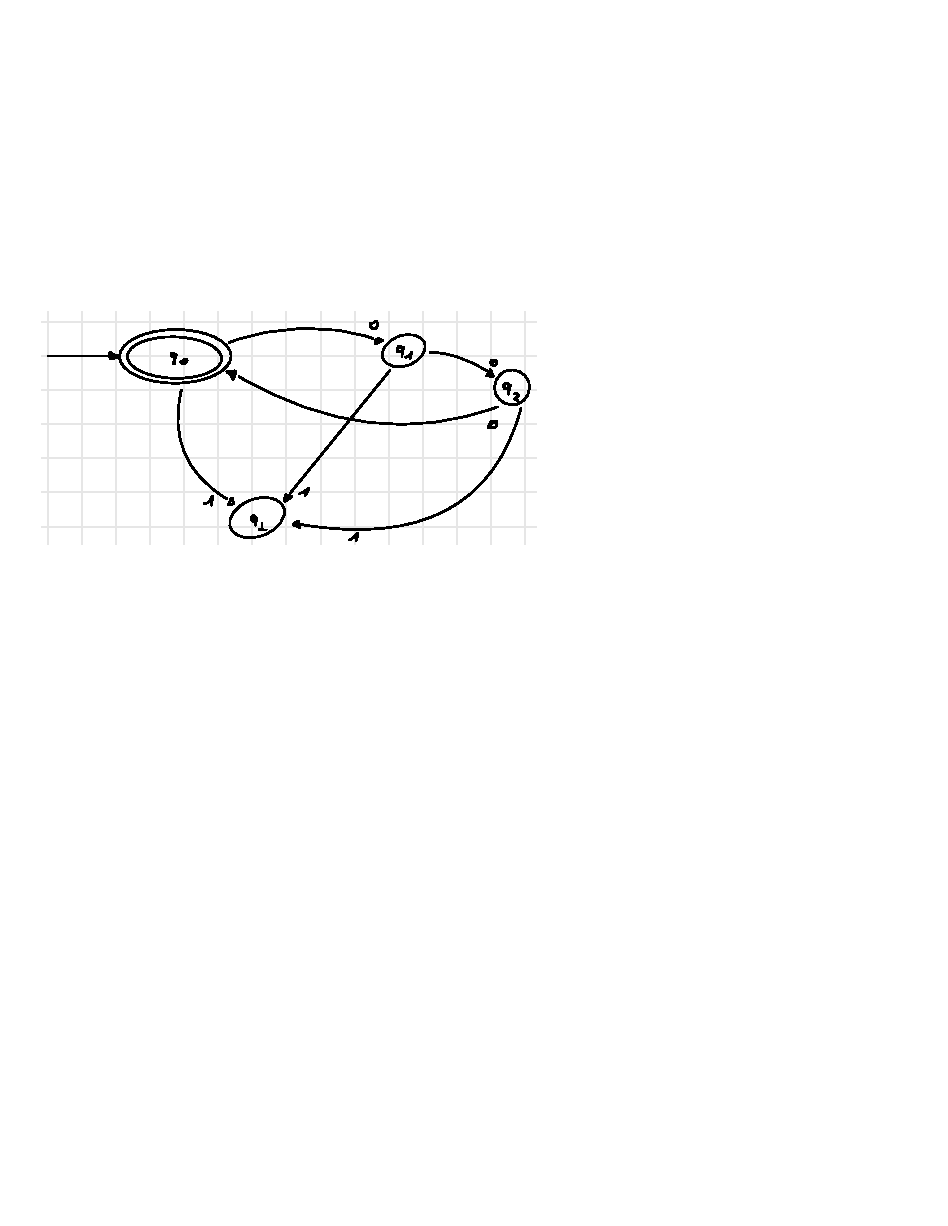
\includegraphics[width=0.8\textwidth]{img/esercitazioni/01_exe3.pdf}
		\caption{Grafo dell'automa a stati finiti deterministico dell'esercizio 3.}\label{ASFD-esercizio_3}
	\end{figure}

	\noindent
	L'unica \textbf{osservazione} da fare riguarda lo stato $q_{\bot}$ è il suo significato. Nell'esercizio 2 a pagina~\pageref{ASFD-esercizio_2} si parla di \dquotes{\textbf{stato pozzo}}, in questo esercizio lo stato $q_{\bot}$ è la stessa identica cosa.
	
	\newpage
	
	\begin{proof}[\textcolor{Blue3}{\textbf{Dimostrazione}}]
		Si vuole dimostrare che $\sigma \in L \iff \delta\left(q_{0}, \sigma\right) \in F$ tramite l'induzione.\newline
		
		\noindent
		\textbf{\underline{Caso base.}}
		
		\begin{enumerate}
			\item $x = \varepsilon \in L \longrightarrow \delta\left(q_{0}, \varepsilon\right) = q_{0} \in F$
			
			\item $x = 0 \notin L \longrightarrow \delta\left(q_{0}, 0\right) = q_{1} \notin F$
			
			\item $x = 00 \notin L \longrightarrow \delta(\underbrace{q_{0}, 0}_{q_{1}} 0) = \delta\left(q_{1}, 0\right) = q_{2} \notin F$
			
			\item $x = 1 \notin L \longrightarrow \delta\left(q_{0}, 1\right) = q_{\bot} \notin F$
		\end{enumerate}
		
		\noindent
		Con il caso base sono stati ricoperti tutti gli stati.\newline
		
		\noindent
		\textbf{\underline{Ipotesi induttiva.}}\newline
		
		\noindent
		Si vuole dimostrare che $\sigma \in L \Longrightarrow \delta\left(q_{0}, \sigma\right) \in F$, allora l'ipotesi induttiva è: se $|x| < n$ allora $x \in L \Longrightarrow \delta\left(q_{0}, x\right) \in F$. Per farlo, si dimostrano le due casistiche classiche:
		
		\begin{itemize}
			\item $x^{'} = x0 \notin L \longrightarrow \delta(\overbrace{q_{0}, x}^{q_{0}} 0) = \delta\left(q_{0}, 0\right) = q_{1} \notin F$
			
			\item $x^{'} = x1 \notin L \longrightarrow \delta(\underbrace{q_{0}, x}_{q_{0}} 1) = \delta\left(q_{0}, 1\right) = q_{\bot} \notin F$
		\end{itemize}
	\end{proof}

	\newpage
	
	\begin{proof}[\textcolor{Blue3}{\textbf{Dimostrazione 2}}]
		Dopo la prima dimostrazione, adesso si vuole dimostrare che $\sigma \notin L \Longrightarrow \delta\left(q_{0}, \sigma\right) \notin F$ tramite l'induzione.\newline
		
		\noindent
		Come caso base si utilizza quello visto nella precedente dimostrazione.\newline
		
		\noindent
		\textbf{\underline{Ipotesi induttiva.}}\newline
		
		\noindent
		Si vuole dimostrare che $\sigma \notin L \Longrightarrow \delta\left(q_{0}, \sigma\right) \notin F$, allora l'ipotesi induttiva è: se $|x| < n$ allora $x \notin L \Longrightarrow \delta\left(q_{0}, x\right) \notin F$. Per farlo, si devono trovare delle casistiche particolari:
		
		\begin{enumerate}[label=\alph*.]
			\item $x = 0^{3\mathbb{N} + 1}$
			
			\item $x = 0^{3\mathbb{N} + 2}$
			
			\item $x = \left\{0\right\}^{n} 1 \left\{0, 1\right\}^{n}$
		\end{enumerate}
		
		\noindent
		Le casistiche \dquotes{generali} in cui una stringa non appartiene al linguaggio, e quindi all'insieme degli stati finali $F$, è quando:
		
		\begin{itemize}
			\item La stringa è formata da una concatenazione di $0$ multipli di $3$ ma aggiungendo $1$ al risultato, quest'ultimo non è più multiplo (caso a);
			
			\item Stessa situazione del punto precedente ma aggiungendo $2$ come valore (caso b);
			
			\item La stringa è formata da una concatenazione di zeri, poi almeno un $1$ e successivamente una serie di concatenazioni di $0$ e/o $1$.
		\end{itemize}
		
		\noindent
		Adesso si procede con la dimostrazione dei vari casi:
		
		\begin{enumerate}[label=\alph*.]
			\item $x = 0^{3\mathbb{N} + 1}$
			\begin{itemize}
				\item $x^{'} = x0 \notin L \longrightarrow \delta(\overbrace{q_{0}, x}^{q_{1}} 0) = \delta\left(q_{1}, 0\right) = q_{2} \notin F$
				\item $x^{'} = x1 \notin L \longrightarrow \delta(\underbrace{q_{0}, x}_{q_{1}} 1) = \delta\left(q_{1}, 1\right) = q_{\bot} \notin F$
			\end{itemize}
			
			\item $x = 0^{3\mathbb{N} + 2}$
			\begin{itemize}
				\item $x^{'} = x0 \in L \longrightarrow \delta(\overbrace{q_{0}, x}^{q_{2}} 0) = \delta\left(q_{2}, 0\right) = q_{0} \in F$
				\item $x^{'} = x1 \notin L \longrightarrow \delta(\underbrace{q_{0}, x}_{q_{2}} 1) = \delta\left(q_{2}, 1\right) = q_{\bot} \notin F$
			\end{itemize}
		
			\item $x = \left\{0\right\}^{n} 1 \left\{0, 1\right\}^{n}$
			\begin{itemize}
				\item $x^{'} = x0 \notin L \longrightarrow \delta(\overbrace{q_{0}, x}^{q_{\bot}} 0) = \delta\left(q_{\bot}, 0\right) = q_{\bot} \notin F$
				\item $x^{'} = x1 \notin L \longrightarrow \delta(\underbrace{q_{0}, x}_{q_{\bot}} 1) = \delta\left(q_{\bot}, 1\right) = q_{\bot} \notin F$
			\end{itemize}
		\end{enumerate}
	\end{proof}

	\newpage

	\noindent
	\textcolor{Red3}{\textbf{\underline{Esercizi con linguaggi e relativi grafi}}}\newline
	
	\noindent
	Di seguito si riportano alcuni linguaggi dati come esercizio ed i relativi grafi.\newline
	
	\noindent
	\textcolor{Red3}{\textbf{Esercizio 4}}\newline
	
	\noindent
	Il linguaggio e l'alfabeto:
	
	\begin{gather*}
		L = \left\{0^{n} 1^{m} \hspace{0.5em} | \hspace{0.5em} n,m > 0\right\} \\
		\Sigma = \left\{0, 1\right\}
	\end{gather*}
	
	\begin{figure}[!htp]
		\centering
		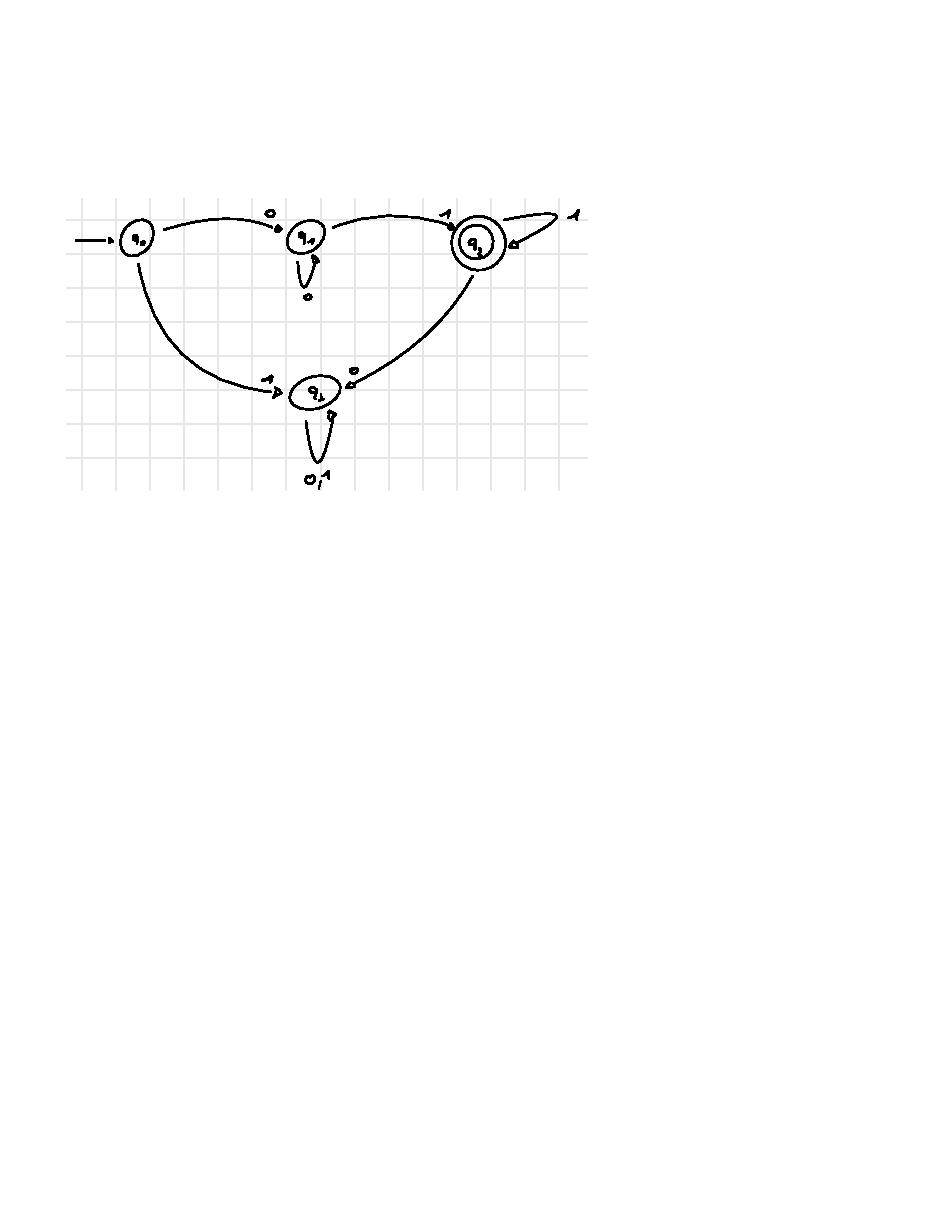
\includegraphics[width=0.8\textwidth]{img/esercitazioni/01_exe4.pdf}
		\caption{Grafo dell'automa a stati finiti deterministico dell'esercizio 4.}\label{ASFD-esercizio_4}
	\end{figure}

	\newpage

	\noindent
	\textcolor{Red3}{\textbf{Esercizio 5}}\newline
	
	\noindent
	Il linguaggio e l'alfabeto:
	
	\begin{gather*}
		L = \left\{x \hspace{0.5em} | \hspace{0.5em} |x_{0}| > 0, |x_{1}| > 1\right\} \\
		\Sigma = \left\{0, 1\right\}
	\end{gather*}
	
	\begin{figure}[!htp]
		\centering
		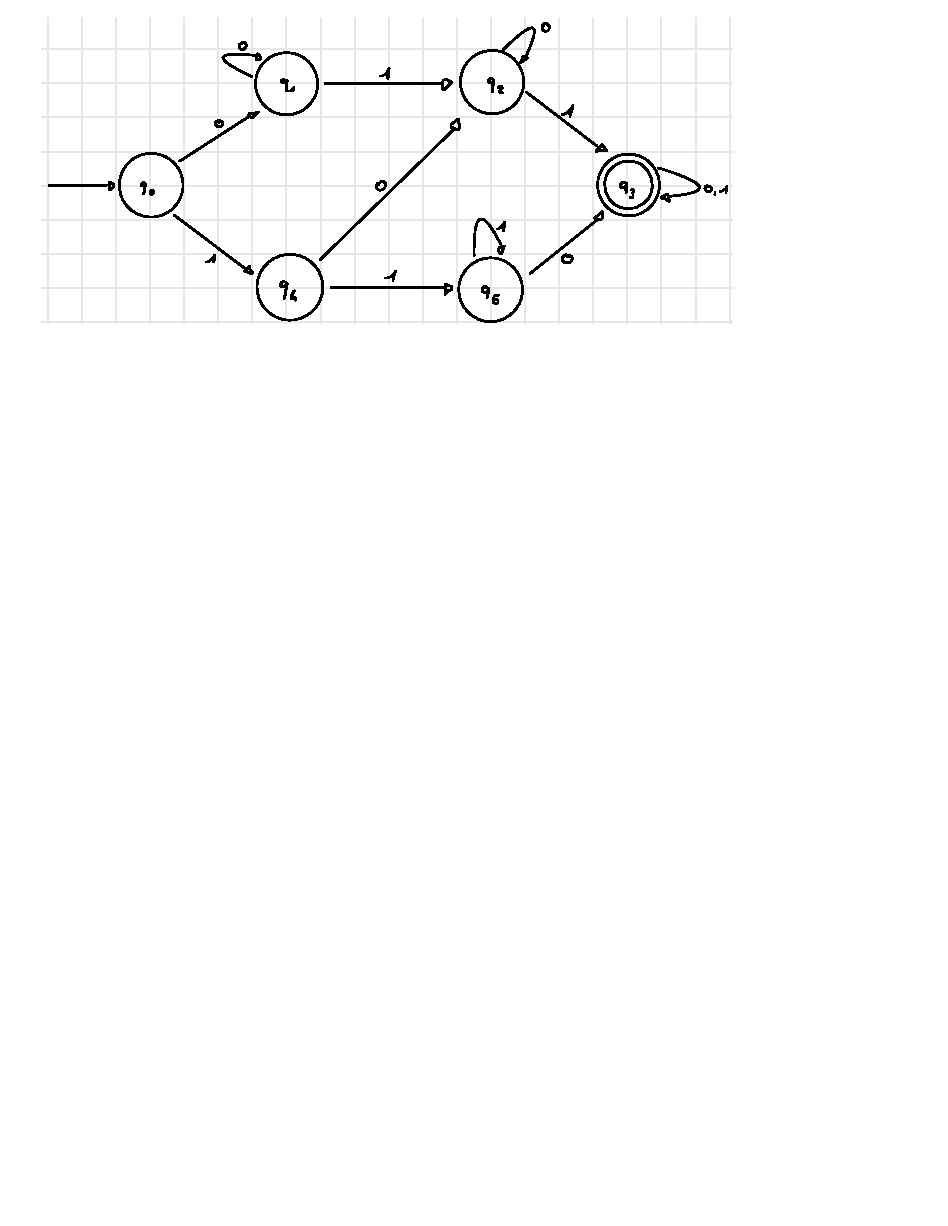
\includegraphics[width=0.8\textwidth]{img/esercitazioni/01_exe5.pdf}
		\caption{Grafo dell'automa a stati finiti deterministico dell'esercizio 5.}\label{ASFD-esercizio_5}
	\end{figure}

	\newpage
	
	\subsubsection{Automi con $\boldsymbol{\varepsilon}$-transizioni ($\boldsymbol{\varepsilon}$-NFA)}
	
	Il terzo tipo di automa che estende il modello non-deterministico precedente ma che è equivalente dal punto di vista dei linguaggi accettati. L'idea è che l'automa compia transizione di stato anche senza leggere alcun simbolo. Questo sarà modellato ammettendo transizioni etichettate $\varepsilon$.
	
	Un \textcolor{Red3}{\textbf{automa a stati finti non deterministico con $\boldsymbol{\varepsilon}$ transizioni}}, brevemente ASFND+$\varepsilon$ oppure $\varepsilon$-NFA, \textcolor{Red3}{\textbf{è una quintupla}}:
	
	\begin{equation*}
		\left\langle Q, \Sigma, \delta, q_{0}, F \right\rangle
	\end{equation*}

	\noindent
	Dove $Q, \Sigma, \delta, q_{0} \text{ e } F \subseteq Q$ sono definiti come per gli automi non-deterministici, mentre la \textbf{\underline{funzione di transizione}} $\delta$ è definita come:
	
	\begin{equation*}
		\delta: Q \times \left(\Sigma \cup \left\{\varepsilon\right\}\right) \longrightarrow P\left(Q\right)
	\end{equation*}

	\noindent
	Ne consegue che la funzione $\overset{\wedge}{\delta}: Q \times \Sigma^{*} \longrightarrow P\left(Q\right)$ nel caso dei $\varepsilon$-NFA risulta più complessa.\newline
	
	\noindent
	Si introduce una nuova \textcolor{Red3}{\textbf{operazione}} chiamata \textcolor{Red3}{\underline{\textbf{$\boldsymbol{\varepsilon}$-chiusura}}} (\textcolor{Red3}{\emph{$\varepsilon$-closure}}) che, applicata ad uno stato, \textcolor{Red3}{\textbf{restituisce l'insieme degli stati raggiungibili da esso (compreso sè stesso) mediante $\boldsymbol{\varepsilon}$-transizioni}}.	Essa non è altro che un insieme di stati:
	
	\begin{equation*}
		\varepsilon\text{-closure}\left(P\right) = \bigcup_{p \in P} \varepsilon\text{-closure}\left(p\right)
	\end{equation*}

	\noindent
	Quindi, la \underline{$\overset{\wedge}{\delta}$ è possibile definirla nel seguente modo}:
	
	\begin{equation*}
		\begin{cases}
			\overset{\wedge}{\delta}\left(q, \varepsilon\right) = \varepsilon\text{-closure}\left(q\right) \\
			\overset{\wedge}{\delta}\left(q, wa\right) = \bigcup_{p \in \hat{\delta}\left(q, w\right)} \varepsilon\text{-closure}\left(\delta\left(p, a\right)\right)
		\end{cases}
	\end{equation*}

	\noindent
	In questo caso è possibile che $\overset{\wedge}{\delta}\left(q, a\right)$ sia diverso da $\delta\left(q, a\right)$. Come, per esempio, nel seguente automa:
	
	\begin{figure}[!htp]
		\centering
		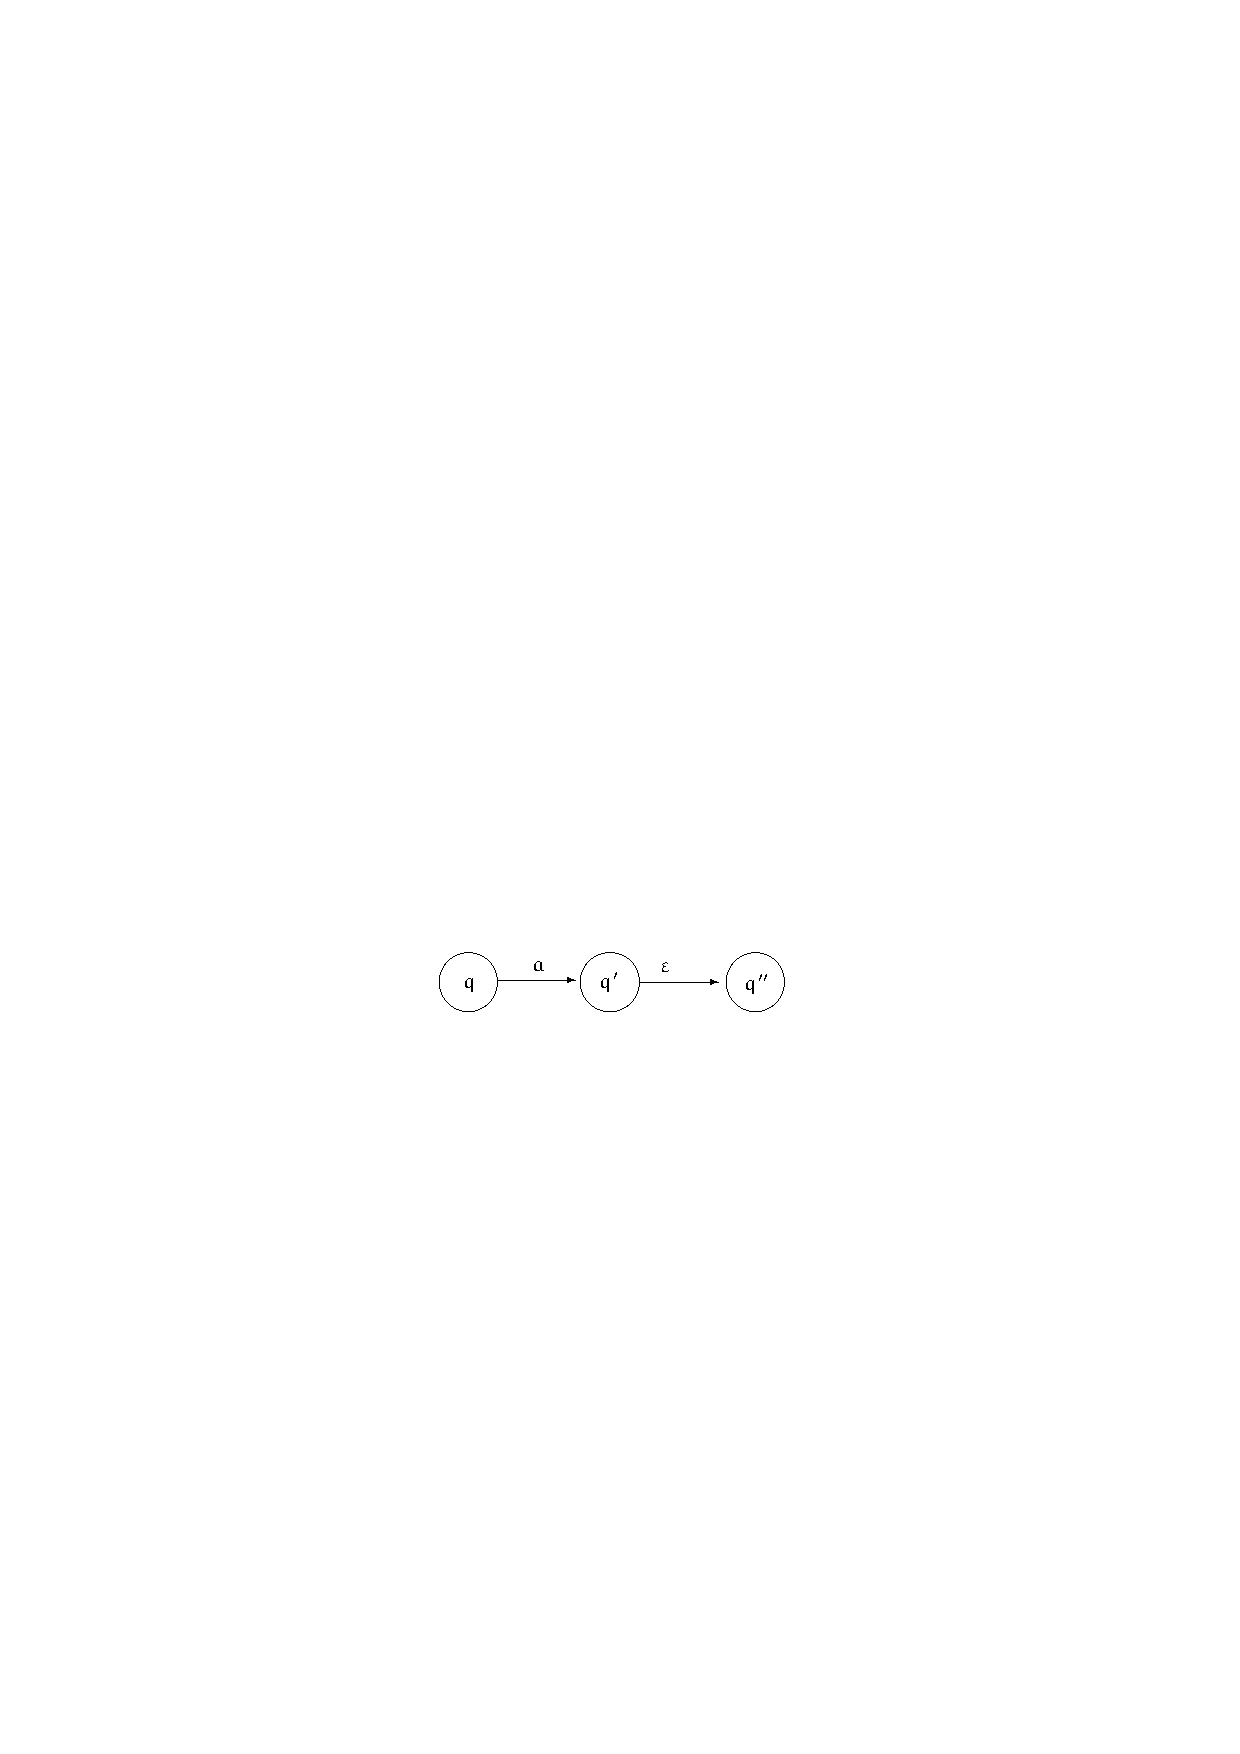
\includegraphics[width=0.5\textwidth]{img/automa_epsilon-transizioni.pdf}
		\caption{Esempio di automa con $\overset{\wedge}{\delta}$ e $\delta$ diversi.}
	\end{figure}

	\noindent
	\dquotes{Consumando} la stringa $a$ si giunge nello stato $q^{'}$: $\delta\left(q, a\right) = \left\{q^{'}\right\}$. Invece, con la stringa $a\varepsilon$ si giunge allo stato $q^{''}$ e si descrive come: $\overset{\wedge}{\delta}\left(q,a\right) = \bigcup_{p \in \hat{\delta}\left(q,\varepsilon\right)} \varepsilon$-closure$\left(\delta\left(p,a\right)\right) = \left\{q^{'}, q^{''}\right\}$.
	
	\noindent
	Infine, si definisce il \textcolor{Red3}{\textbf{linguaggio accettato dall'automa}}:
	
	\begin{equation*}
		L\left(M\right) = \left\{x \in \Sigma^{*} \: \left| \: \hat{\delta}\left(q_{0}, x\right) \cap F \ne \emptyset\right.\right\}
	\end{equation*}

	\noindent
	E inoltre $\overset{\wedge}{\delta}\left(q,x\right) = \varepsilon$-closure $\left(\overset{\wedge}{\delta}\left(q,x\right)\right)$.
	
	\subsubsection{Teorema dell'equivalenza di $\boldsymbol{\varepsilon}$-NFA e NFA}
	
	\textbf{Obbiettivo:} con il seguente teorema si dimostra che la classe dei linguaggi riconosciuti dagli automi $\varepsilon$-NFA non estende propriamente quella dei linguaggi riconosciuti da automi NFA.
	
	\begin{theorem}[\textbf{Equivalenza}]
		Sia una quintupla di un automa a stati finiti non-deterministico $\varepsilon$ ($\varepsilon$-NFA):
		
		\begin{equation*}
			M = \langle Q, \Sigma, \delta, q_{0}, F \rangle
		\end{equation*}
	
		\noindent
		Allora esiste un automa a stati finiti non-deterministico (NFA) $M^{'}$ tale che $L\left(M\right) = L\left(M^{'}\right)$.
	\end{theorem}

	\begin{proof}[\textbf{Dimostrazione}]
		Si definisce l'automa a stati finiti non-deterministico $M^{'}$ con la quintupla:
		
		\begin{equation*}
			M^{'} = \langle Q^{'}, \Sigma^{'}, \delta^{'}, q_{0}^{'}, F^{'} \rangle
		\end{equation*}
	
		\noindent
		Con le caratteristiche simili alla NFA:
		
		\begin{itemize}
			\item $Q^{'} = Q$
			\item $\Sigma^{'} = \Sigma$
			\item $q_{0}^{'} = q_{0}$
			\item $F^{'} =
				\begin{cases}
					F \cup \left(q_{0}\right) 	& \text{se } \varepsilon\text{-closure}\left(q_{0}\right) \cap F \ne \emptyset \\
					F 							& \text{altrimenti}
				\end{cases}$
			\item $\delta^{'} \left(q,a\right) = \overset{\wedge}{\delta}\left(q,a\right)$
		\end{itemize}
	
		\noindent
		Si osservi che nel sistema degli stati finiti $F$, l'unione con lo stato iniziale $q_{0}$ produce uno stato finito (se l'intersezione non è nulla!).
		
		\noindent
		L'\textbf{\underline{obbiettivo}} è dimostrare che siano uguali:
		
		\begin{equation*}
			\overset{\wedge}{\delta}\left(q_{0}, x\right) \cap F \ne \emptyset \iff \overset{\wedge}{\delta^{'}}\left(q_{0}, x\right) \cap F^{'} \ne \emptyset
		\end{equation*}
		
		\noindent
		Quindi, in altri termini:
		
		\begin{equation*}
			\forall x \in \Sigma^{*} \longrightarrow \overset{\wedge}{\delta}\left(q_{0}, x\right) = \overset{\wedge}{\delta^{'}}\left(q_{0}, x\right) \hspace{2em} \text{per } |x|\ge 1
		\end{equation*}
	
		\noindent
		\textbf{\underline{Caso base.}}\newline
		
		\noindent
		Entrambe hanno l'operazione $\varepsilon$-closure.
		
		\newpage
		
		\noindent
		\textbf{\underline{Passo induttivo.}}
		
		\begin{gather*}
			\overset{\wedge}{\delta^{'}}(q_{0}, \overbrace{xa}^{n+1}) = \bigcup_{p \in \hat{\delta^{'}}\left(q_{0}, x\right)} \delta^{'}\left(p, a\right) \\
			\xrightarrow{\text{per definizione}}\bigcup_{p \in \hat{\delta^{'}} \left(q_{0}, x\right)} \overset{\wedge}{\delta} \left(p, a\right) \\
			\xrightarrow{\text{per induzione}}\bigcup_{p \in \hat{\delta}\left(q_{0}, x\right)} \overset{\wedge}{\delta}\left(p, a\right) \\
			\xrightarrow{\text{applicando l'operazione}}\bigcup_{p \in \hat{\delta}\left(q_{0}, a\right)} \varepsilon\text{-closure}\left(\delta\left(p, a\right)\right) \\
			\xrightarrow{\text{si conclude}} \overset{\wedge}{\delta}\left(q_{0}, xa\right)
		\end{gather*}
	
		\noindent
		Si \textbf{\underline{conclude la dimostrazione}} verificando graficamente che $F = F^{'}$. Per farlo, si pensi al caso in cui $F^{'} \ne F$, ovvero un caso impossibile. Questo perché lo stato $q_{0}$ è \textbf{per definizione} contenuto sia nell'insieme $F$, sia nell'insieme $F^{'}$ (dimostrazione eseguita sopra).
		
		Quindi, \textbf{lo stato $q_{0}$, se presente in uno dei due insiemi, sarà sicuramente presente anche nell'altro}, come si vede dall'immagine~\ref{dimostrazione:equivalenza insieme}.
		
		\begin{figure}[!htp]
			\centering
			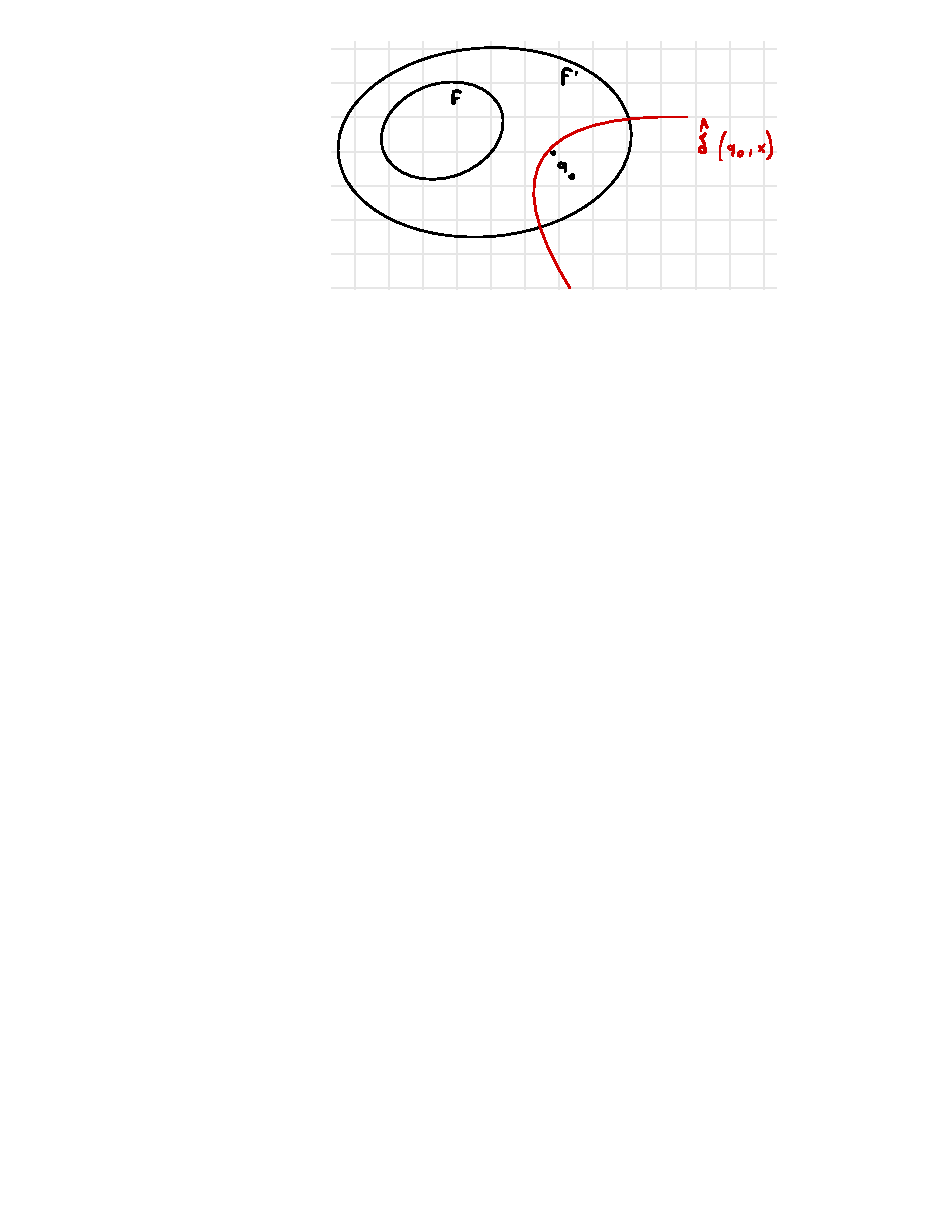
\includegraphics[width=0.5\textwidth]{img/teorema_equivalenza1.pdf}
			\caption{Dimostrazione grafica per evidenziare l'impossibilità della presenza dello stato $q_{0}$ solamente in un insieme.}
			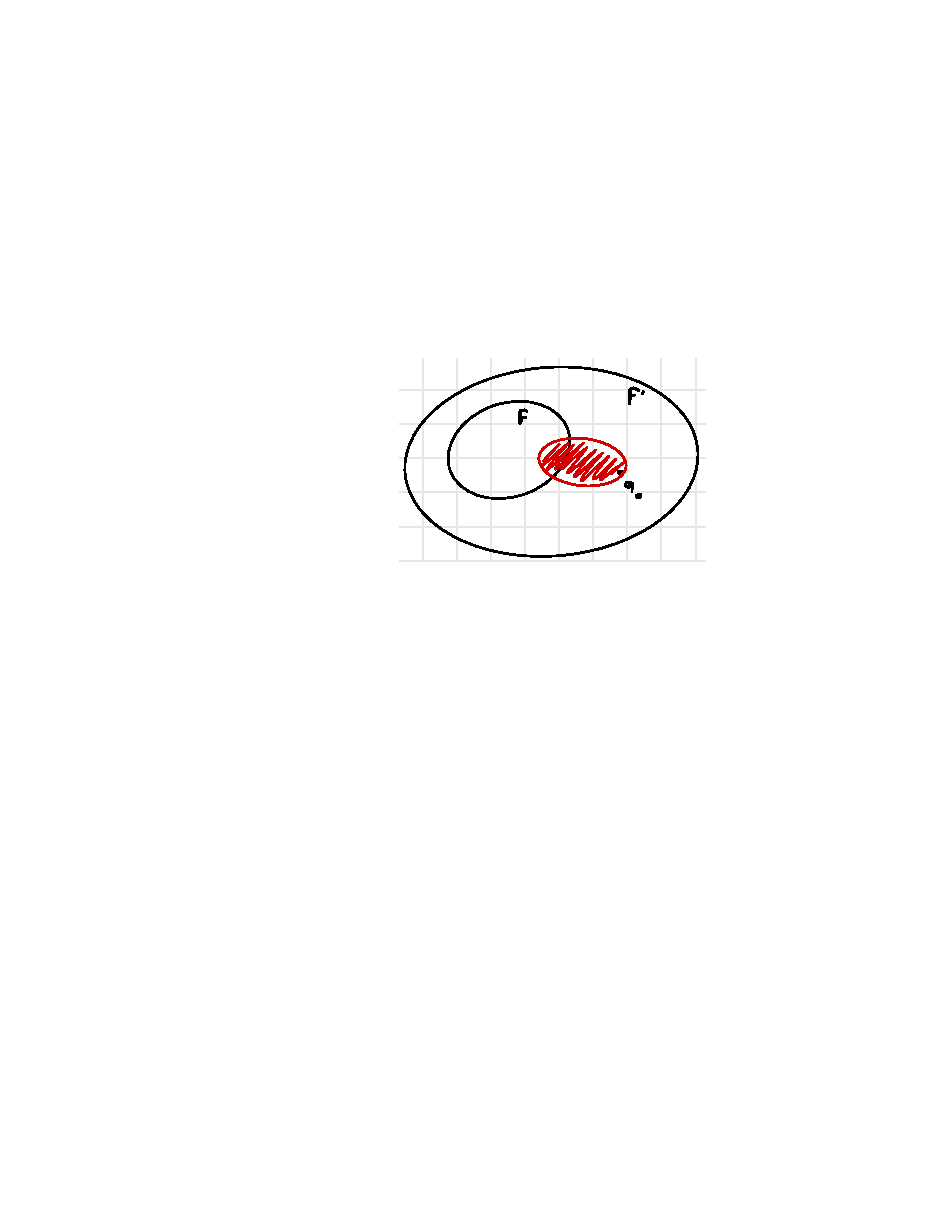
\includegraphics[width=0.5\textwidth]{img/teorema_equivalenza2.pdf}
			\caption{Dimostrazione grafica della corretta rappresentazione dei due insiemi e dello stato $q_{0}$.}\label{dimostrazione:equivalenza insieme}
		\end{figure}
	\end{proof}


	\section{Espressioni regolari}
	
	\subsection{Espressioni regolari}
	
	Sia $\Sigma$ un alfabeto, si definiscono \textcolor{Red3}{\textbf{espressioni regolari su $\Sigma$}} e gli \textbf{insiemi} che esse denotano tramite le seguenti caratteristiche:
	
	\begin{enumerate}[label=\Roman*.]
		\item $\emptyset$ è una espressione regolare che indica l'\textbf{insieme vuoto};
		
		\item $\varepsilon$ è una espressione regolare che indica l'\textbf{insieme $\left\{\varepsilon\right\}$};
		
		\item Per ogni simbolo $a \in \Sigma$, $a$ è una espressione regola che indica l'\textbf{insieme $\left\{a\right\}$};
		
		\item Se $r$ e $s$ sono espressioni regolari che denotano rispettivamente gli insiemi $R$ e $S$, allora:
			\begin{itemize}[label=-]
				\item $\left(r + s\right)$ denota l'insieme $R \cup S$
				\item $\left(rs\right)$ denota l'insieme $R \cap S$ oppure con un'altra notazione $RS$
				\item $\left(r^{*}\right)$ denota l'insieme $R^{*}$
			\end{itemize}
	\end{enumerate}

	\noindent
	Se $r$ è una espressione regolare, si indica con $L\left(r\right)$ il linguaggio denotato con $r$, ovvero l'insieme di stringhe di $\Sigma^{*}$ che essa denota. Inoltre, varrà l'eguaglianza $r = s$ se e solo se $L\left(r\right) = L\left(s\right)$.\newline
	
	\noindent
	Quindi, \textbf{\underline{riassumendo la definizione}}:
	
	\begin{itemize}[label=\ding{42}]
		\item $L\left(\emptyset\right) = \emptyset$
		\item $L\left(\varepsilon\right) = \left\{\varepsilon\right\}$
		\item $L\left(a\right) = \left\{a\right\}$
		\item $L\left(r+s\right) = L\left(r\right) \cup L\left(s\right)$
		\item $L\left(r \cdot s\right) = L\left(r\right) \cdot L\left(s\right)$
		\item $L\left(r^{*}\right) = L\left(r\right)^{*}$
	\end{itemize}

	\noindent
	\textcolor{Green4}{\textbf{Esempi:}}
	
	\begin{itemize}[label=-]
		\item $\left\{a^{n} b^{m} c^{h} \: \left| \: m,n,h \ge 0 \right.\right\} \longrightarrow a^{*} b^{*} c^{*}$
		
		\item $\left\{a^{n} b^{m} c^{h} \: \left| \: m,n,h > 0 \right.\right\} \longrightarrow aa^{*} bb^{*} cc^{*}$
	\end{itemize}

	\noindent
	\textcolor{Red3}{\textbf{\underline{Proprietà}}}
	
	\begin{itemize}[label=\ding{72}]
		\item $e_{1} + \left(e_{2} + e_{3}\right) = e_{1}\cdot e_{2} + e_{1} \cdot e_{3}$
		
		\item $\left(e_{1} + e_{2}\right) \cdot e_{3} = e_{1} \cdot e_{3} + e_{2} \cdot e_{3}$
		
		\item $e_{1} + \left(e_{2} + e_{3}\right) = \left(e_{1} + e_{2}\right) + e_{3}$
		
		\item $e_{1} \cdot \left(e_{2} \cdot e_{3}\right) = \left(e_{1} \cdot e_{2}\right) \cdot e_{3}$
		
		\item $e \cdot \varepsilon = \varepsilon \cdot e = e$
		
		\item $e \cdot \emptyset = \emptyset \cdot e = \emptyset$
		
		\item $e + e = e$
		
		\item $\emptyset^{*} = \varepsilon$
	\end{itemize}

	\newpage
	
	\subsubsection{Teorema McNaughton \& Yamamada (1960) - Equivalenza tra DFA e ER}

	\begin{theorem}[\textbf{McNaughton \& Yamamada}]
		Sia $r$ una espressione regolare, allora esiste una macchina $M$ (automa) a stati finiti non-deterministico + $\varepsilon$ tale che $L\left(M\right) = L\left(r\right)$. Più formale:\footnote{ER = espressione regolare.}
		
		\begin{equation*}
			r \in ER \Longrightarrow L\left(r\right)
		\end{equation*}
	\end{theorem}
	
	\begin{proof}[\textbf{Dimostrazione}]
		Si dimostra che esiste un automa a stati finiti non-deterministico + $\varepsilon$ tale che $L\left(r\right) = L\left(M\right)$. Formalmente:
		
		\begin{equation*}
			\exists M \underbrace{ASFND+\varepsilon}_{\varepsilon-NFA} \text{ t.c. } L\left(r\right) = L\left(M\right)
		\end{equation*}
	
		\noindent
		Per farlo, si hanno i seguenti tre casi base.\newline
		
		\noindent
		\textbf{\underline{Caso base.}}
		
		\begin{itemize}
			\item L'automa $\varepsilon$ è composto da un solo stato finito:
				\begin{figure}[!htp]
					\centering
					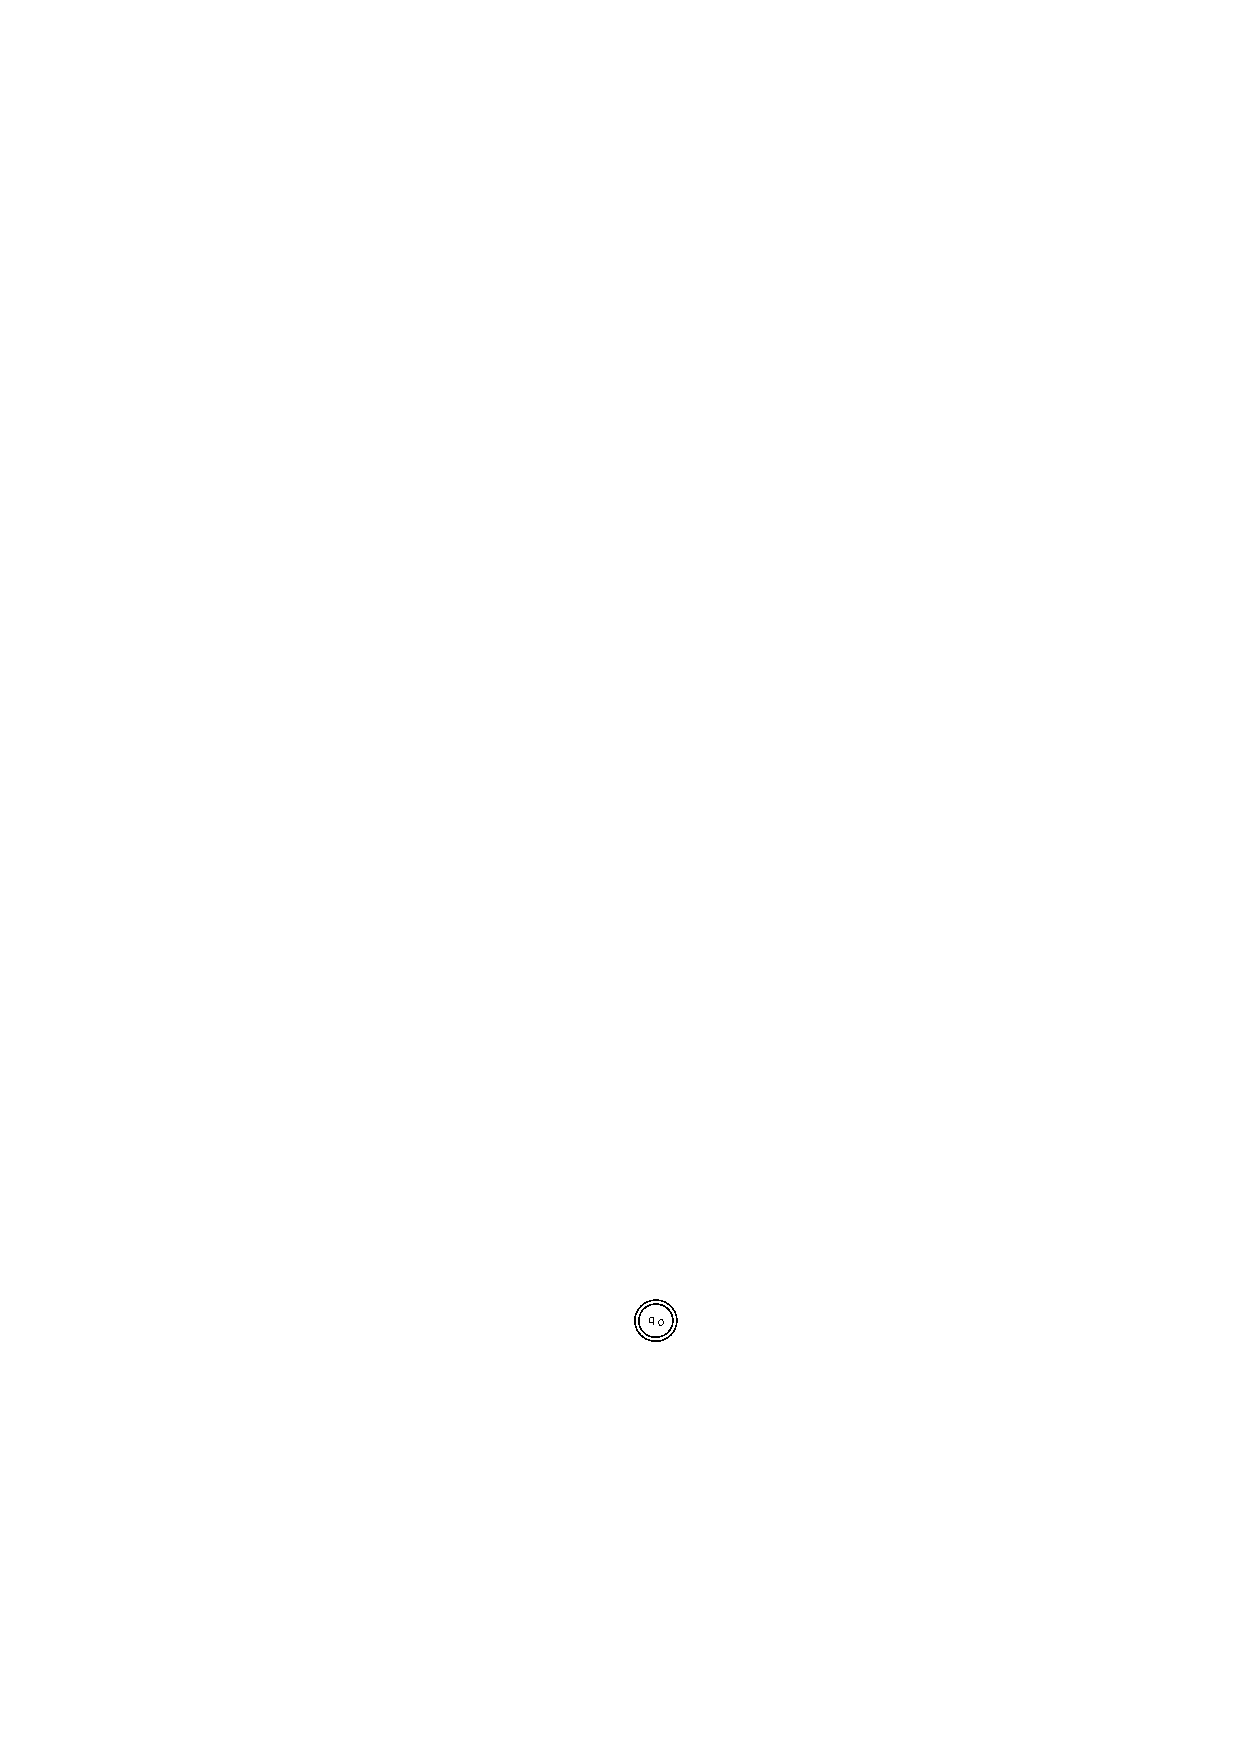
\includegraphics[width=0.13\textwidth]{img/teorema_McN-Yamada1.pdf}
				\end{figure}
			
			\item L'automa $\emptyset$ è composto da uno stato iniziale e uno stato finale che non viene mai raggiunto:
				\begin{figure}[!htp]
					\centering
					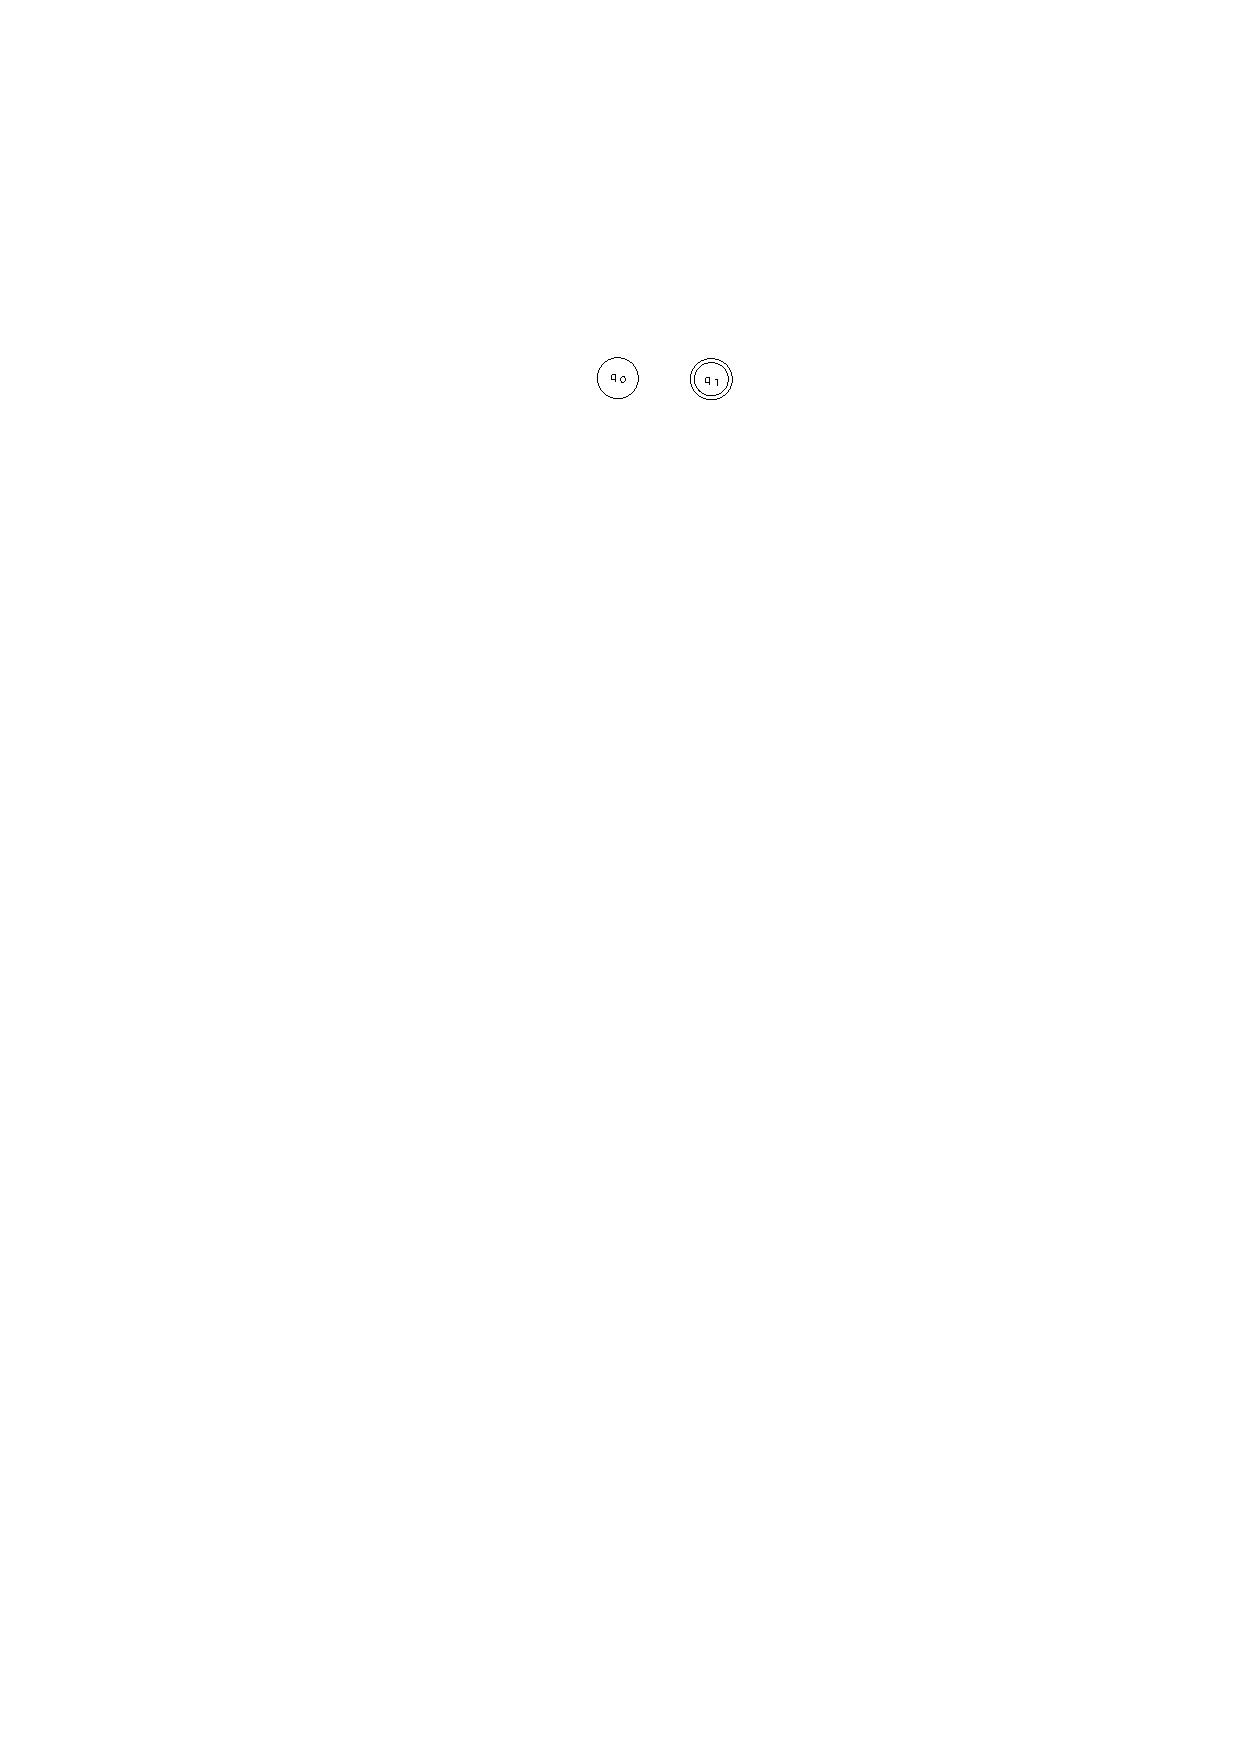
\includegraphics[width=0.3\textwidth]{img/teorema_McN-Yamada2.pdf}
				\end{figure}
			
			\item L'automa $a$ ha uno stato iniziale che accetta una stringa $a$, la quale la porta allo stato finale:
				\begin{figure}[!htp]
				\centering
				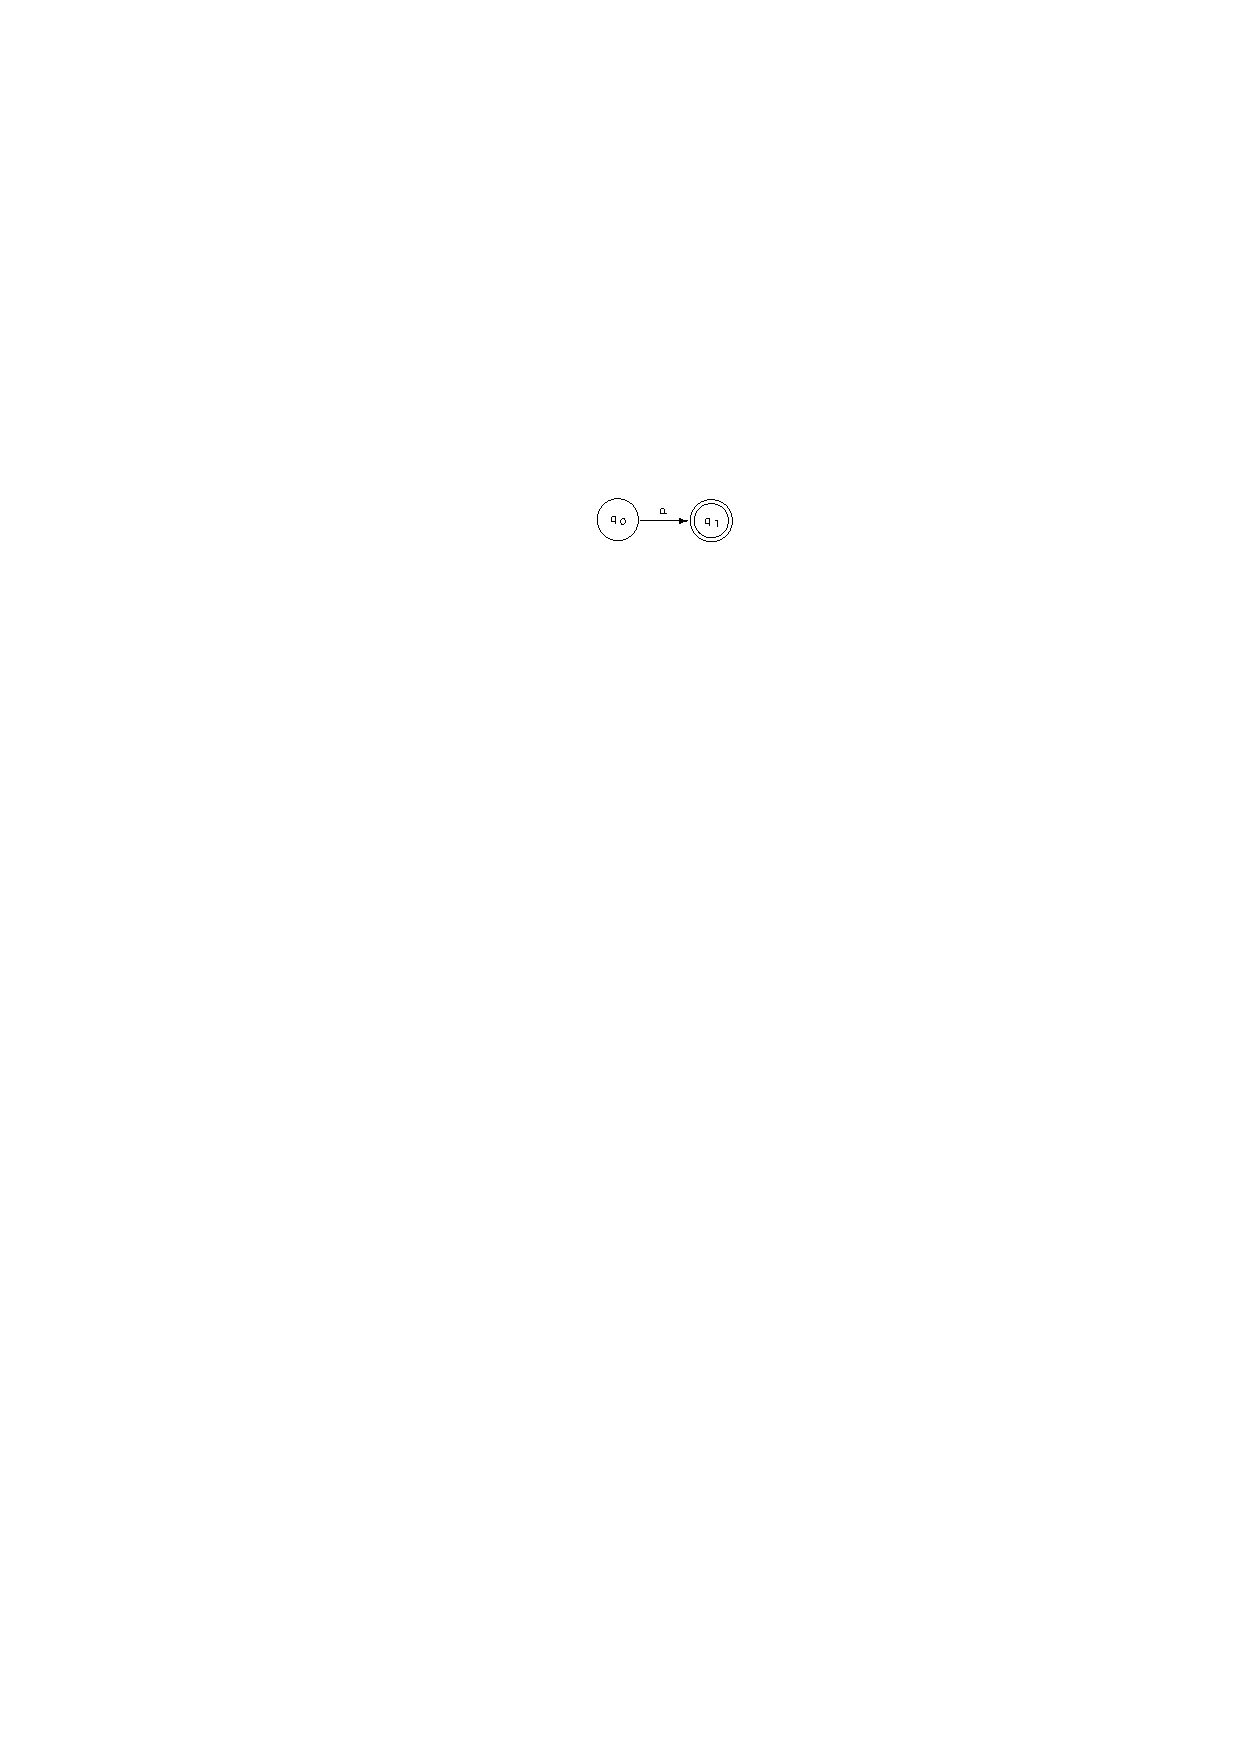
\includegraphics[width=0.3\textwidth]{img/teorema_McN-Yamada3.pdf}
			\end{figure}
		\end{itemize}
	
		\newpage
	
		\noindent
		\textbf{\underline{Passo induttivo.}}\newline
		
		\noindent
		Ipotizzando che $r$ ed $s$ siano espressioni regolari $r,s \in ER$ e si creano due macchine per le espressioni regolari: $L\left(r\right) = M_{1}$ e $L\left(s\right) = M_{2}$. Si analizzano tre casi:
		
		\begin{itemize}
			\item $r + s$. Questo automa riconosce il linguaggio $L\left(r\right) \cup L\left(s\right)$
				\begin{figure}[!htp]
					\centering
					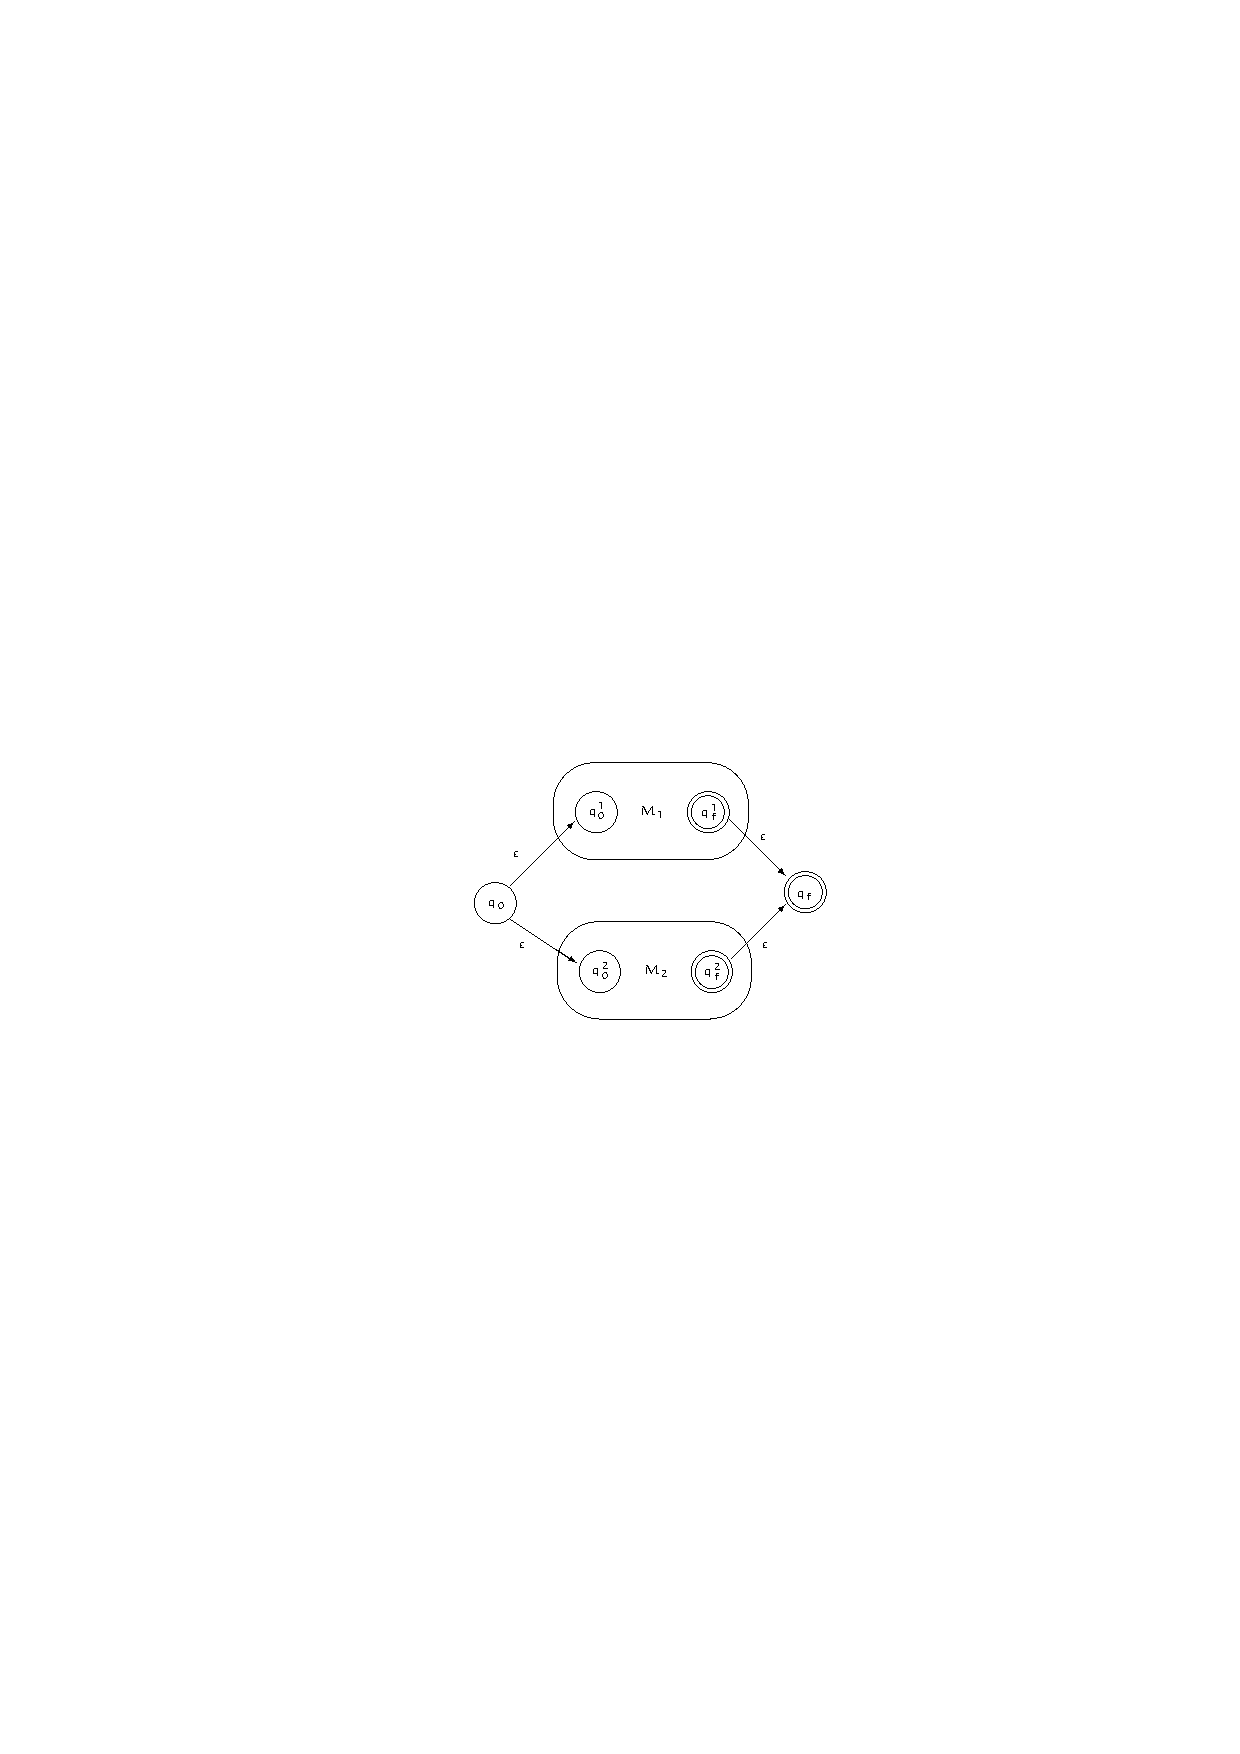
\includegraphics[width=0.7\textwidth]{img/teorema_McN-Yamada4.pdf}
				\end{figure}
			
			\item $r \cdot s$. Questo automa riconosce il linguaggio $L\left(r\right) \cap L\left(s\right)$
				\begin{figure}[!htp]
					\centering
					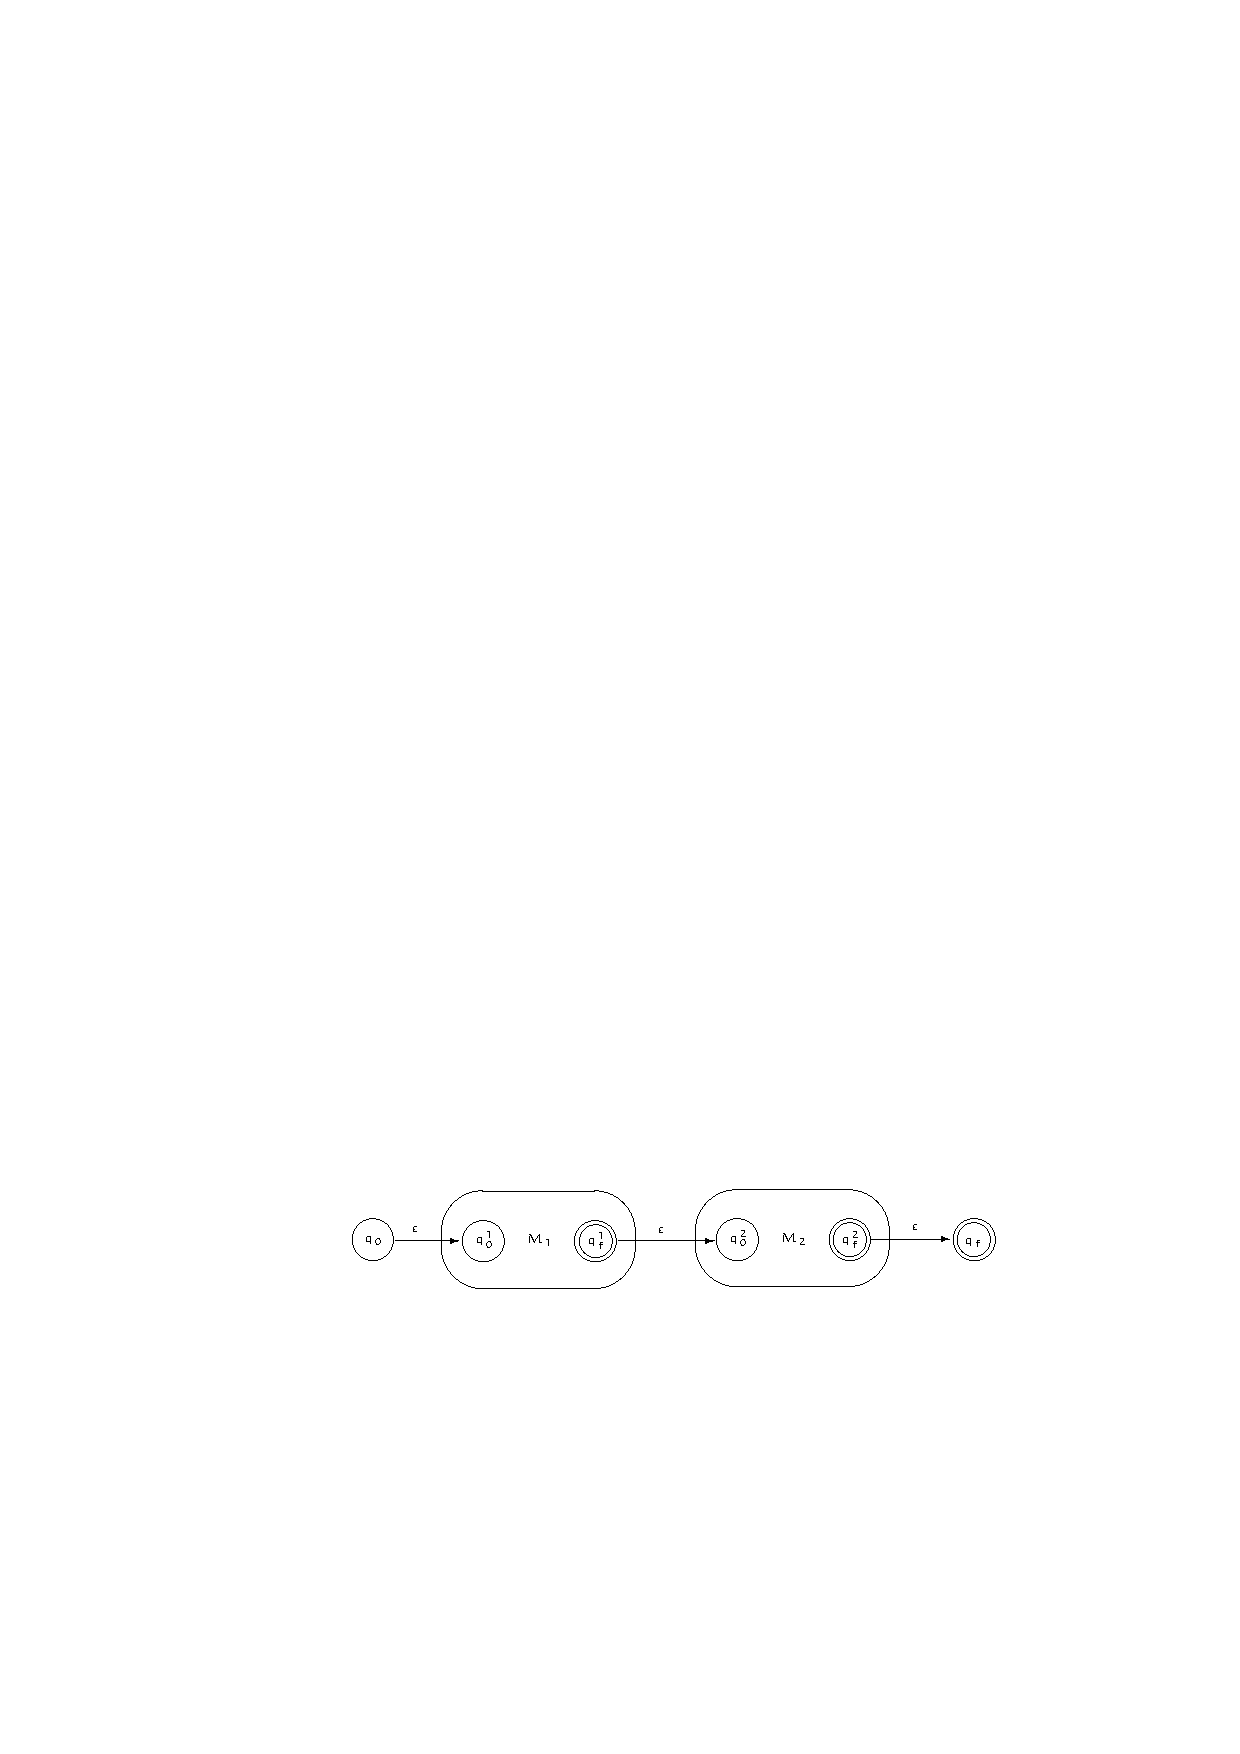
\includegraphics[width=1\textwidth]{img/teorema_McN-Yamada5.pdf}
				\end{figure}
			
			\item $r^{*}$. Questo automa riconosce il linguaggio $L\left(r\right)^{*}$
				\begin{figure}[!htp]
					\centering
					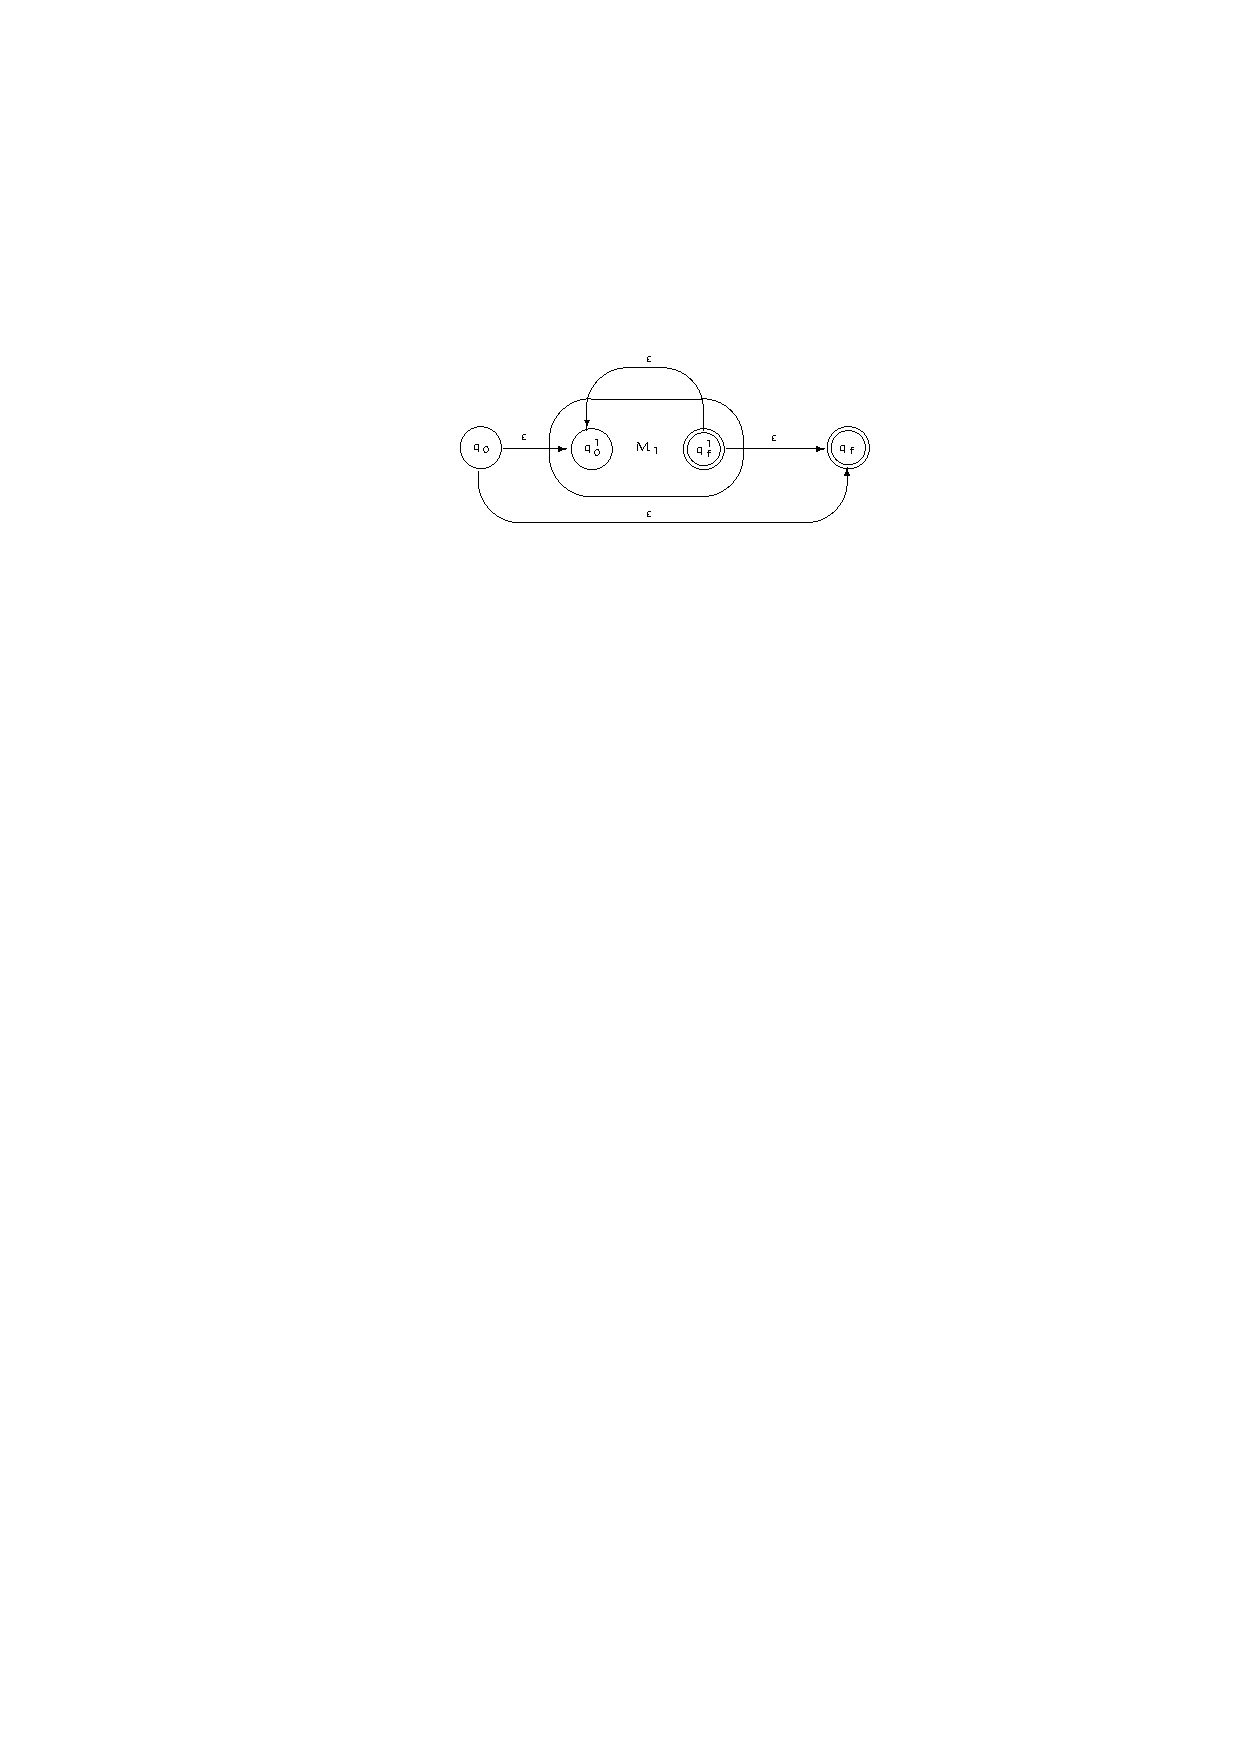
\includegraphics[width=0.8\textwidth]{img/teorema_McN-Yamada6.pdf}
				\end{figure}
		\end{itemize}
	\end{proof}

	\newpage

	\subsubsection{Proprietà di chiusura}
	
	\begin{theorem}[\textcolor{Red3}{\textbf{Proprietà di chiusura}}]
		I linguaggi regolari sono \textbf{\underline{chiusi}} \textbf{rispetto alle operazioni di unione, concatenazione e chiusura di Kleene}.
	\end{theorem}
	\begin{proof}[\textcolor{Green4}{\textbf{Dimostrazione}}]
		Immediata dalla definizione di espressione regolare e dal Teorema di McNaughton \& Yamada (1960).
	\end{proof}

	\vspace{2em}

	\begin{theorem}[\textcolor{Red3}{\textbf{Complementazione}}]
		I \textbf{linguaggi regolari} sono \textbf{chiusi rispetto all'operazione di complementazione}. Formalmente:
		
		\begin{equation*}
			\text{Se } L \subseteq \Sigma^{*} \text{ è regolare, anche } \bar{L} = \Sigma^{*} \setminus L \text{ è regolare}
		\end{equation*}
	\end{theorem}
	\begin{proof}[\textcolor{Green4}{\textbf{Dimostrazione}}]
		Sia $M = \langle Q, \Sigma^{'}, \delta, q_{0}, F \rangle$ l'automa a stati finiti deterministico (DFA) che riconosce il linguaggio $L$. Si assuma che $\Sigma^{'} = \Sigma$, allora $M^{'} = \langle Q, \Sigma, \delta, q_{0}, Q \setminus F \rangle$ riconosce il linguaggio $\bar{L}^{'}$.
	\end{proof}

	\vspace{2em}

	\begin{theorem}[\textcolor{Red3}{\textbf{Intersezione}}]
		\textbf{I linguaggi regolari sono chiusi rispetto all'intersezione}.
	\end{theorem}
	\begin{proof}[\textcolor{Green4}{\textbf{Dimostrazione}}]
		Immediata dal fatto che $L_{1} \cap L_{2} = \overline{\left(\overline{L_{1}} \cup \overline{L_{2}}\right)}$
	\end{proof}

	\newpage
	
	\section{Proprietà dei linguaggi regolari}
	
	\subsection{Teorema di Myhill-Nerode (1957-58)}
	
	Prima di introdurre il teorema di Myhill-Nerode (1957-58), si espongono alcuni concetti base.\newline
	
	\noindent
	Dato un insieme $S$, una relazione di equivalenza $R \subseteq S \times S$ induce univocamente una partizione di $S = S_{1} \cup S_{2} \cup \cdots$ ove per ogni $i$ si ha $S_{i} \ne \emptyset$ e per ogni $i, j$ con $i \ne j$ si ha che:
	
	\begin{enumerate}[label=\Roman*]
		\item $S_{i} \cap S_{j} = \emptyset$
		
		\item $\left(\forall a, b \in S_{i}\right): a \: R \: b$
		
		\item $\left(\forall a \in S_{i}\right)\left(\forall b \in S_{j}\right): \lnot \left(a \: R \: b\right)$
	\end{enumerate}
	
	\noindent
	Le varie $S_{i}$ sono dette \textcolor{Red3}{\textbf{\underline{classi di equivalenza}}}. La notazione è la seguente (caso in cui $a$ appartenga alla classe di equivalenza $S_{i}$):
	
	\begin{equation*}
		a \in S_{i} \longrightarrow \left[a\right]_{R}
	\end{equation*}\newline

	\noindent
	Se $S$ è partizionato in un numero finito di classi $S_{1} \cup S_{2} \cup \cdots \cup S_{k}$ allora $R$ viene detto \textcolor{Red3}{\textbf{\underline{indice finito}}} su $S$.\newline
	
	\noindent
	Date due relazioni $R_{1}$ e $R_{2}$ sullo stesso insieme $S$, $R_{1}$ è un \textcolor{Red3}{\textbf{\underline{raffinamento}}} di $R_{2}$ se ogni classe di equivalenza della partizione indotta da $R_{1}$ è sottoinsieme di qualche classe di equivalenza della partizione indotta da $R_{2}$.\newline
	
	\noindent
	\textcolor{Green4}{\textbf{\underline{Per esempio}}}, se $S = \left\{2, 3, 4, 5\right\}, P_{1} = \left\{\left\{2, 3, 5\right\}, 4\right\}$ e $P_{2} = \left\{\left\{2\right\}, \left\{3, 5\right\}, \left\{4\right\}\right\}$ denotano le partizioni di $S$ ottenute a partire dalle seguenti relazioni:
	
	\begin{gather*}
		\left(R_{1}\right) \hspace{1em} x \: R_{1} \: y \iff x \text{ e } y \text{ sono entrambi primi o uguali tra loro} \\
		\left(R_{2}\right) \hspace{1em} x \: R_{2} \: y \iff x \text{ e } y \text{ sono entrambi primi e dispari, o uguali tra loro}
	\end{gather*}

	\noindent
	Allora $R_{2}$ è un \emph{\textbf{raffinamento}} di $R_{1}$.\newline
	
	\newpage
	
	\noindent
	Ad ogni linguaggio $L \subseteq \Sigma$ è possibile associare una relazione di tipo $R_{L} \subseteq \Sigma^{*} \times \Sigma^{*}$ definita nel seguente modo:
	
	\begin{equation}\label{relazione sul linguaggio}
		x \: R_{L} \: y \iff \left(\forall z \in \Sigma^{*}\right) \left(xz \in L \leftrightarrow yz \in L \right)
	\end{equation}
	
	\noindent
	Questa definizione viene chiamata \textcolor{Red3}{\textbf{\underline{relazione sul linguaggio}}}.\newline
	
	\noindent
	Analogamente, se $M = \left\langle Q, \Sigma, \delta, q_{0}, F \right\rangle$ è una macchina a stati finiti deterministica (DFA), è possibile associare una relazione di tipo $R_{M} \subseteq \Sigma^{*} \times \Sigma^{*}$ definita come:
	
	\begin{equation}\label{relazione sull'automa}
		x \: R_{M} \: y \iff \hat{\delta}\left(q_{0}, x \right) = \hat{\delta} \left(q_{0}, y\right)
	\end{equation}
	
	\noindent
	Questa definizione viene chiamata \textcolor{Red3}{\textbf{\underline{relazione sull'automa/macchina}}}. Inoltre, li linguaggio $L_{q} = \left\{x \in \Sigma^{*} \: : \: \hat{\delta}\left(q_{0}, x\right) = q\right\}$ è associato allo stato $q$ dell'automa. È evidente che le classi di equivalenza $R_{M}$ sono esattamente i linguaggi associati ad ogni stato dell'automa $M$.\newline
	
	\begin{lemma}[\textbf{Relazioni di equivalenza}]
		La relazione sul linguaggio e la relazione sull'automa (o macchina) vengono chiamate \textcolor{Red3}{\textbf{\underline{relazioni di equivalenza}}}.
	\end{lemma}
	\:\newline
	
	\noindent
	Infine, una relazione $R \subseteq \Sigma^{*} \times \Sigma^{*}$ che gode della seguente proprietà:
	
	\begin{equation*}
		x \: R \: y \xlongrightarrow{implica} \left(\forall z \in \Sigma^{*}\right) \left(xz \: R \: yz\right)
	\end{equation*}

	\noindent
	(la relazione) si chiama \textcolor{Red3}{\textbf{\underline{invariante a destra}}} rispetto alla concatenazione. Quindi sia la \textbf{relazione sul linguaggio che sull'automa/macchina è invariante a destra}.
	
	\newpage
	
	\begin{proof}[\textcolor{Red3}{\textbf{Dimostrazione invariante a destra - Relazione sull'automa/macchina}}]
		La relazione sull'automa/macchina è invariante destra poiché aggiungendo una lettera $z$ a $x$, il comportamento è identico anche per $y$ (dimostrazione verbale, non matematica).
	\end{proof}

	\begin{proof}[\textcolor{Red3}{\textbf{Dimostrazione invariante a destra - Relazione sul linguaggio}}]
		Si ipotizzi per assurdo che data la relazione $x \: R \: y$, l'espressione che se ne deriva sia \textbf{\emph{falsa}}, cioè:
		
		\begin{equation*}
			\forall z \in \Sigma^{*}  \: : \: xz \: R \: yz
		\end{equation*}
	
		\noindent
		Se ne deriva che dunque esiste:
		
		\begin{equation*}
			\exists z \in \Sigma^{*} \: : \: \bcancel{xz \: R_{L} \: yz}
		\end{equation*}
	
		\noindent
		Ovvero che la relazione è falsa.
		
		\noindent
		Dalla relazione sul linguaggio:
		
		\begin{equation*}
			\exists w \in \Sigma^{*} \: : \: x\underbrace{zw}_{z^{'}} \in L, \:\: y\underbrace{zw}_{z^{'}} \in L
		\end{equation*}
	
		\noindent
		Allora per assurdo si ottiene:
		
		\begin{equation*}
			xz^{'} \in L, \:\: yz^{'} \notin L \Longrightarrow x \: R_{L} \: y
		\end{equation*}
	\end{proof}
	
	\newpage
	
	\begin{theorem}[\textbf{Myhill-Nerode, 1957-58}]
		Le seguenti affermazioni si equivalgono:
		
		\begin{enumerate}
			\item $L \subseteq \Sigma^{*}$ è regolare;
			
			\item $L$ è l'unione di classi di equivalenza su $\Sigma^{*}$ indotte da una relazione invariante a destra di indice finito\footnote{Con indice finito si intende che l'insieme viene \emph{partizionato} in classi finite.};
			
			\item $R_{L}$ è di indice finito.
		\end{enumerate}
	\end{theorem}

	\begin{proof}[\textbf{Dimostrazione}]
		La dimostrazione avviene per implicazione, cioè che $(1) \Rightarrow (2), (2) \Rightarrow (3)$ e $(3) \Rightarrow (1)$.

		\begin{center}
			\item[\ding{42}] $(1) \Rightarrow (2)$
		\end{center}
		
		\noindent
		Sia $L$ un linguaggio regolare, come da definizione 1. È dunque ammesso un automa a stati finiti deterministico (ASFD o DFA) con la quintupla $M = \left\langle Q, \Sigma, \delta, q_{0}, F \right\rangle$ tale per cui il linguaggio regolare è uguale al linguaggio dell'automa $L = L\left(M\right)$. L'automa è di \textbf{indice finito} poiché il numero di stati è finito.\newline
		
		\noindent
		Per definizione di linguaggio riconosciuto da un automa, si ha la seguente uguaglianza:
		
		\begin{equation*}
			L = \bigcup_{q \in F} \overbrace{\left\{x \in \Sigma^{*} \: \left| \: \hat{\delta}\left(q_{0}, x\right) = q \right.\right\}}^{L_{q}}
		\end{equation*}
	
		\noindent
		Dato che la relazione sull'automa $M$ ($R_{M}$) è invariante a destra, l'espressione $L_{q}$ rappresenta i vari insiemi che costituiscono le classi di equivalenza della partizione indotta da $R_{M}$.\newline
		
		\noindent
		In termini matematici:
		
		\begin{gather*}
			\text{Se } x \in \Sigma^{*} : \left[x\right]_{R_{M}} = L_{q} \hspace{1em} \text{per un qualsiasi } q \in Q \\
			|Q| < w \Rightarrow L = \bigcup_{q \in F} L_{q}
		\end{gather*}
	
		\noindent
		Si ricorda che $\left[x\right]_{R_{M}}$ indica la classe di equivalenza.
		
		\newpage
		
		\begin{center}
			\item[\ding{42}] $(2) \Rightarrow (3)$
		\end{center}
		
		\noindent
		Assumendo che il punto 2 del teorema sia vero, si vuole dimostrare che l'indice è finito. Ovvero, ogni relazione di equivalenza $R$ che soddisfa il punto 2 è un raffinamento di $R_{L}$.
		
		Sia $x \in \Sigma^{*}$, si vuole dimostrare che $\left[x\right]_{R} \subseteq \left[x\right]_{R_{L}}$, cioè che il numero degli elementi in $R_{L}$ è maggiore o uguale di $R$.\newline
		
		\noindent
		\textbf{\underline{Ipotesi induttiva:}} si assuma che $y \in \left[x\right]_{R}$ sia vera (N.B. $\Rightarrow y \in \left[x\right]_{R_{L}}$).
		
		\noindent
		Dall'ipotesi induttiva e dal fatto che la relazione $R$ è invariante a destra per ipotesi, allora:
		
		\begin{equation*}
			\forall z \in \Sigma^{*} : xz \: R \: yz
		\end{equation*}
	
		\noindent
		Quindi, dato che $L$ è l'unione delle classi di equivalenza di $R$:
		
		\begin{equation*}
			L = \left[x_{1}\right]_{R} \cup \cdots \cup \left[x_{n}\right]_{R}
		\end{equation*}
	
		\noindent
		Ciò implica che ogni qualvolta, in generale, si ha una relazione del tipo:
		
		\begin{equation*}
			v \: R \: w \Longrightarrow v \in L \iff w \in L
		\end{equation*}
	
		\noindent
		Pertanto, sostituendo i termini generali $v$ e $w$ rispettivamente con $xz$ e $yz$:
		
		\begin{equation*}
			\forall z \in \Sigma^{*} : \underbrace{xz}_{v} \in L \iff \underbrace{yz}_{w} \in L \coloneqq x \: R_{L} \: y
		\end{equation*}
	
		\noindent
		La relazione sul linguaggio $R_{L}$ tra $x$ e $y$ viene ricavata per definizione (come nell'equazione~\ref{relazione sul linguaggio}). Si può riscrivere anche come:
		
		\begin{equation*}
			y \in \left[x\right]_{R_{L}}
		\end{equation*}
	
		\noindent
		Essendo la relazione $R$ un raffinamento della relazione sul linguaggio $R_{L}$, l'indice di $R_{L}$ è minore di quello di $R$, che per ipotesi è finito. Infatti, essendo un raffinamento, sicuramente in $R$ l'indice sarà maggiore. Si conclude che $R_{L}$ ha indice finito.
		
		\newpage
		
		\begin{center}
			\item[\ding{42}] $(3) \Rightarrow (1)$
		\end{center}
		
		\noindent
		Assumendo che la relazione sul linguaggio abbia un indice finito, si deduce che esiste un automa a stati finiti deterministico tale che $L = L\left(M\right)$. Quindi, si costruisce la macchina nel seguente modo:
		
		\begin{equation*}
			\text{ASFD (DFA) } M^{'} = \left\langle Q^{'}, \Sigma^{'}, \delta^{'}, q_{0}^{'}, F^{'} \right\rangle \text{ che riconosce } L
		\end{equation*}
		
		\begin{enumerate}[label=\Roman*.]
			\item $Q^{'}$ è l'insieme (finito per ipotesi) di classi di equivalenza di $R_{L}$, formalmente: $\left\{\left[x\right]_{R_{L}} \: \left| \: x \in \Sigma^{*}\right.\right\}$;
			
			\item $\Sigma^{'}$ è lo stesso di $L$, cioè un alfabeto finito;
			
			\item $\delta^{'} \left(\left[x\right], a\right) = \left[xa\right]$ dato che $R_{L}$ è invariante a destra, la definizione vale indipendentemente dalla scelta di $x$;
			
			\item $q_{0}^{'} = \left[\varepsilon\right]$;
			
			\item $F^{'} = \left\{\left[x\right]_{R_{L}} \: \left| \: x \in L \right.\right\}$.
		\end{enumerate}
		
		\noindent
		Mostrando che $L\left(M^{'}\right) = L$ si termina la dimostrazione.\newline
		
		\noindent
		Allora si suppone che esiste una $y$:
		
		\begin{equation*}
			\forall y \in \Sigma^{*} : \hat{\delta}\left(\left[x\right]_{R_{L}}, y\right) = \left[x y\right]_{R_{L}}
		\end{equation*}
		
		\noindent
		E con le diverse cardinalità di $y$ si dimostra che:
		
		\begin{itemize}
			\item $|y| = 0 \iff y = \varepsilon : \hat{\delta} \left(\left[x\right]_{R_{L}}, \varepsilon\right) = \left[x\right]_{R_{L}} = \left[x\varepsilon\right]_{R_{L}}$
			
			\item $|y| \ge 0 : \hat{\delta}\left(\left[x\right]_{R_{L}}, ya\right) = \delta\left(\hat{\delta}\left(\left[x\right]_{R_{L}}, y\right), a\right) = \delta\left(\left[xy\right]_{R_{L}}, a\right) = \left[xya\right]_{R_{L}}$
		\end{itemize}
		
		\noindent
		Analogamente, si ha lo stesso ragionamento:
		
		\begin{equation*}
			\hat{\delta^{'}}\left(q_{0}^{'}, x\right) = \hat{\delta^{'}}\left(\left[\varepsilon\right], x\right) = \left[\varepsilon, x\right] = \left[x\right]
		\end{equation*}
		
		\noindent
		Dunque si conclude la dimostrazione:
		
		\begin{equation*}
			x \in L\left(M^{'}\right) \iff \hat{\delta^{'}}\left(q_{0}^{'}, x\right) \in F^{'} \iff \left[x\right] \in F^{'} \iff x \in L
		\end{equation*}
		
		\noindent
		Che tradotto vorrebbe dire che $x$ appartiene al linguaggio dell'automa $M^{'}$ se e solo se la transizione dallo stato iniziale $q_{0}$ consumando $x$ sia uno stato finale, cioè appartenente a $F$, se e solo se la classe di equivalenza $x$ della relazione sul linguaggio $R_{L}$ appartiene all'insieme degli stati finali se e solo se $x$ appartiene al linguaggio.
	\end{proof}

	\newpage
	
	\subsection{Pumping Lemma}
	
	Il pumping lemma è un \textbf{metodo utilizzato per dimostrare che un linguaggio \emph{non} è regolare}.
	
	\begin{lemma}[\textbf{Bar-Hillel, Perles, Shamir, 1961}]
		Sia $L$ un linguaggio regolare. Allora esiste una costante $n \in \mathbb{N}$ tale che per ogni $z \in L$ tale che $|z| \ge n$ esistono tre stringhe $u, v, w$ tali che:
		
		\begin{enumerate}
			\item $z = uvw$ con $u,v,w \in \Sigma^{*}$;
			\item $|uv| \le n$;
			\item $|v| > 0$, cioè non può essere vuota;
			\item per ogni $i \ge 0$ vale che $u v^{i} w \in L$ o in forma più matematica: $\forall i \ge 0: uv^{i}w \in L$.
		\end{enumerate}
	\end{lemma}

	\begin{proof}[\textcolor{Green4}{\textbf{Dimostrazione grafica}}]
		Data un automa a stati finiti deterministico (ASFD o DFA) con la quintupla $M = \left\langle Q, \Sigma, \delta, q_{0}, F \right\rangle$ e con il linguaggio $L\left(M\right) = L$.\newline
		Data la stringa $z \in L = L\left(M\right)$ e con la lunghezza $n = |Q| + 5$.\footnote{Il numero $5$ è casuale, si potrebbe prendere anche $1$, l'importante è che la lunghezza di $n$ sia più grande.}\newline
		
		\noindent
		Quindi, l'automa si crea nel seguente modo:
		
		\begin{figure}[!htp]
			\centering
			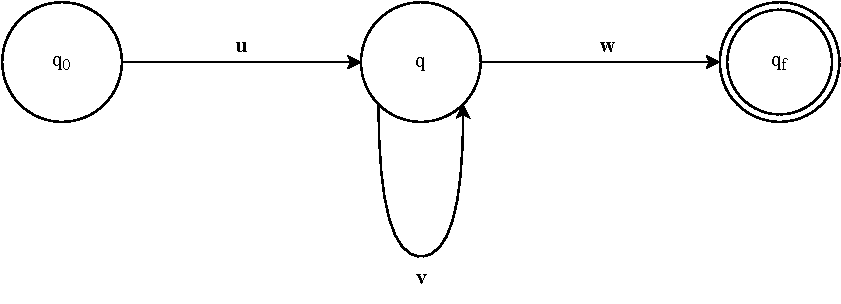
\includegraphics[width=1\textwidth]{img/lemma_pumping1.pdf}
			\caption{Automa a stati finiti deterministico.}
		\end{figure}
	
		\noindent
		\textbf{\underline{Punto 1, dimostrazione $z = uvw$ con $u,v,w \in \Sigma^{*}$.}}
		
		\noindent
		La dimostrazione è immediata poiché si esegue creando l'automa della dimostrazione. Infatti, nell'automa si vede chiaramente la distinzione delle tre parti della stringa, ovvero la $u$, la $v$ e la $w$.\newline
		
		\noindent
		\textbf{\underline{Punto 2, dimostrazione $|uv| \le n$.}}
		
		\noindent
		La cardinalità di $uv$ deve essere minore o uguale ad $n$ poiché in caso contrario dovrebbe esserci un altro stato tra $q_{0}$ e $q$. L'aggiunta di uno stato renderebbe la lunghezza della stringa più lunga di $n$.
		
		\newpage
		
		\noindent
		\textbf{\underline{Punto 3, dimostrazione $|v| > 0$, cioè non può essere vuota.}}
		
		\noindent
		È abbastanza chiara la dimostrazione poiché se $v$ non fosse maggiore di zero, lo stato non si ripeterebbe almeno una volta e questo andrebbe in contrasto con il punto $4$ del \emph{Pumping Lemma} in cui la $v$ si ripete almeno una volta (con $i = 0$ si ha una ripetizione di $v$).\newline
		
		\noindent
		\textbf{\underline{Punto 4, dimostrazione $\forall i \ge 0: uv^{i}w \in L$.}}
		
		\noindent
		Anche questa dimostrazione è immediata. Guardando l'automa a stati finiti è evidente che, dato un numero indefinito di $v$, si arriverà comunque allo stato finale una volta ricevuto il simbolo $w$ nello stato $q$.
	\end{proof}

	\vspace{2em}
	
	Si osservi come il lemma asserisca la veridicità di una \textbf{formula logica} che afferma: per ogni linguaggio $L$, se $L$ è regolare, allora vale
	
	\begin{equation}\label{Pumping lemma}
		\exists n \in \mathbb{N} \: \forall z
		\left(
		\begin{matrix}
			\left(z \in L \land |z| \ge z\right) \Rightarrow \exists u, v, w \\
			\addlinespace
			\left( z = uvw \land |uv| \le n \land |v| > 0 \land \forall i \left(i \in \mathbb{N} \Rightarrow uv^{i}w \in L\right) \right)
		\end{matrix}
		\right)
	\end{equation}
	
	Come detto all'inizio del paragrafo, l'\textbf{\underline{obbiettivo}} dell'utilizzo del Pumping Lemma è dimostrare che un dato linguaggio non è regolare. Per farlo, si assume che $L$ non sia regolare e si deve mostrare che vale la negazione della formula~\eqref{Pumping lemma}, quindi:
	
	\begin{equation}
		\forall n \in \mathbb{N} \: \exists z
		\left(
		\begin{matrix}
			z \in L \land |z| \ge n \: \land \\
			\addlinespace
			\forall u, v, w
			\left(
			\begin{matrix}
				z = uvw \land |uv| \le n \land |v| > 0 \\
				\addlinespace
				\Rightarrow \exists i \left(i \in \mathbb{N} \land uv^{i}w \notin L \right)
			\end{matrix}
			\right)
		\end{matrix}
		\right)
	\end{equation}\newline
	
	\noindent
	\textcolor{Green4}{\textbf{\emph{Esempi di linguaggi non regolari}}}\newline
	
	\noindent
	I seguenti linguaggi sono irregolari:
	
	\begin{itemize}
		\item $L = \left\{a^{n} b^{n} \: \left| \: n \ge 0 \right.\right\}$
		
		\item $L = \left\{a^{n^{2}} \: \left| \: n \ge 1 \right.\right\}$
	\end{itemize}

	\noindent
	Al contrario, un linguaggio regolare è per esempio:
	
	\begin{equation*}
		L = \left\{a^{2n} \: \left| \: n \ge 0 \right.\right\}
	\end{equation*}

	\newpage
	
	\subsubsection[\textcolor{Red3}{Esercizi da esame}]{Esercizi da esame}
	
	\textcolor{Red3}{\textbf{\underline{Esercizio 1}}}\newline
	
	\noindent
	I dati dell'esercizio sono i seguenti:
	
	\begin{equation*}
		L = \left\{1^{k} \: 0^{i} \: 1^{i} \: 0^{j} \: 1^{j} \: 0^{k} \: \left| \: i,j,k \ge 0 \right.\right\}
	\end{equation*}\newline
	
	\noindent
	\textcolor{Green4}{\textbf{\emph{Risoluzione.}}}\newline
	
	\noindent
	Per prima cosa si analizza il linguaggio per verificare se è regolare o no. Nel caso in cui lo fosse, si eseguono le procedure ampiamente spiegate al paragrafo~\ref{Esercizi da esame - ASFD / linguaggi regolari}. Tuttavia, in caso contrario, come in questo esercizio, si applica il Pumping Lemma.
	
	Perché questo linguaggio non è regolare? Per capirlo basta vedere la sequenza accettata dal linguaggio. Infatti, in questo caso il numero di zeri (indice $i$), per esempio, deve essere uguale al numero di uni (sempre indice $i$). Per sapere il numero esatto di ripetizioni di zeri, per poi concatenare lo stesso numero di volte gli uni, è necessaria una memoria. Dunque, il linguaggio non è regolare.
	
	Questo ragionamento può essere esteso sia per $1$ e $0$ con indice $k$, sia per $0$ e $1$ con indice $j$.
	
	\begin{proof}[\textcolor{Blue3}{\textbf{Dimostrazione}}]
		Per qualsiasi $n$ si prende una stringa $z$ la quale rappresenti il caso limite, ovvero quella situazione che non è gestibile da un ASFD senza memoria:
		
		\begin{equation*}
			\forall n : z = 1^{n} 0^{n} \hspace{1em} \text{con } n = 0 \text{ e } i,j = 0	
		\end{equation*}
	
		\noindent
		Grazie al Pumping Lemma è noto per definizione che $z = uvw$ e $|uv| \le n$. Inoltre, la stringa con l'indice $i$ del Pumping Lemma diventa:
		
		\begin{equation*}
			z^{'} = u v^{i} w = 1^{n + |v|\left(i - 1\right)} \: 0^{n}
		\end{equation*}
		
		\noindent
		Se ne deduce che data la stringa $z$, la sua suddivisione è simile alla seguente figura:
		
		\begin{figure}[!htp]
			\centering
			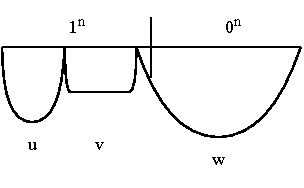
\includegraphics[width=0.4\textwidth]{img/lemma_pumping_ex1.pdf}
			\caption{Rappresentazione della stringa $z$.}
		\end{figure}
		
		\noindent
		Si ipotizzi una $i$ per rendere l'espressione più semplice da manipolare. Quindi, con $i = 2$ l'espressione diventa:
		
		\begin{equation*}
			z^{'} = u v^{i} w = 1^{n + |v|\left(i - 1\right)} \: 0^{n} =1^{n + |v|\left(2 - 1\right)} \: 0^{n} = 1^{n + |v|} \: 0^{n}
		\end{equation*}
	
		\noindent
		Si analizzano gli esponenti per renderli uguali poiché gli $1$ devono essere uguali, come quantità, agli $0$:
		
		\begin{equation*}
			n + |v| = n \xrightarrow{approssimando} \cancel{n} + |v| = \cancel{n}
		\end{equation*}
	
		\noindent
		Se ne conclude che $|v| = 0$ e che per assurdo $z \notin L$.
	\end{proof}

	\newpage
	
	\noindent
	\textcolor{Red3}{\textbf{\underline{Esercizio 2}}}\newline
	
	\noindent
	I dati dell'esercizio sono i seguenti:
	
	\begin{equation*}
		L = \left\{0^{m} \: 1^{n} \: 0^{k} \: 1^{2k} \: \left| \: m,n,k \in \mathbb{N} \right.\right\}
	\end{equation*}\newline
	
	\noindent
	\textcolor{Green4}{\textbf{\emph{Risoluzione.}}}\newline
	
	\noindent
	Il linguaggio potrebbe sembrare regolare, ma se si separa la parte che non provoca una \dquotes{rottura}, si può osservare che serve una memoria e dunque è irregolare:
	
	\begin{equation*}
		L^{'} = \left(0^{k} \: 1^{2k} \: \left| \: k \in \mathbb{N} \right.\right)
	\end{equation*}

	\begin{proof}[\textcolor{Blue3}{\textbf{Dimostrazione}}]
		Per qualsiasi $k$ che faccia parte dei naturali, si cerca una stringa limite:
		
		\begin{equation*}
			\forall k \in \mathbb{N} : z = 0^{k} \: 1^{2k}
		\end{equation*}
	
		\noindent
		Il pumping lemma assicura che sia vero che $z = uvw$, $|uv| \le k$ e infine $|v| > 0$.\newline
		
		\noindent
		Si sceglie una $i$, ma prima si costruisce la stringa $z^{'}$:
		
		\begin{equation*}
			z^{'} = u v^{i} w = 0^{k} \: 1^{2k} = 0^{k + |v|\left(i-1\right)} \: 1^{2k}
		\end{equation*}
	
		\noindent
		Si applica sempre la $i = 2$ e $z^{'} \in L$, cioè deve appartenere al linguaggio. Questo è vero solamente se:
		
		\begin{equation*}
			z^{'} \in L \iff 2k = 2 \left(k+|v|\right)\left(i-1\right)
		\end{equation*}
		
		\noindent
		Gli esponenti, per essere uguali, necessitano di una manipolazione. Infatti, il valore $2$ è stato aggiunto anche a destra poiché il numero di $1$ è il doppio degli zeri e dunque, per uguagliarli, si aggiunge un $2$ al numero di zeri. Si sostituisce anche la $i$ e si eseguono le semplificazioni:
		
		\begin{equation*}
			\begin{array}{cl}
				& 2k = 2 \left(k+|v|\right)\left(2-1\right) \\
				\rightarrow & \cancel{2k} = \cancel{2k} + 2 |v| \\
				\rightarrow & |v| = 0
			\end{array}
		\end{equation*}
	
		\noindent
		La conclusione per assurdo si conclude con $|v| = 0$, che non soddisfa il Pumping Lemma e dunque dimostra che il linguaggio non è regolare ma $z^{'} \in L^{'}$.
	\end{proof}

	\newpage
	
	\noindent
	\textcolor{Red3}{\textbf{\underline{Esercizio 3}}}\newline
	
	\noindent
	I dati dell'esercizio sono i seguenti:
	
	\begin{equation*}
		L = \left\{\omega \: \omega^{R} \: \left| \: \omega \in \left\{0,1\right\}^{*} \right.\right\}
	\end{equation*}\newline

	\noindent
	N.B. con $\omega^{R}$ si intende l'inversione (\emph{reverse}) della stringa.\newline
	
	\noindent
	\textcolor{Green4}{\textbf{\emph{Risoluzione.}}}\newline
	
	\noindent
	Il linguaggio è irregolare poiché per capire eseguire l'inversione di una stringa, si deve salvare la stringa originale.
	
	\begin{proof}[\textcolor{Blue3}{\textbf{Dimostrazione}}]
		Per qualsiasi $n$ appartenente ai naturali, si considera la stringa limite $z$:
		
		\begin{equation*}
			\forall n \in \mathbb{N} : z = \underbrace{0^{n} \: 1}_{\omega} \: \underbrace{1 \: 0^{n}}_{\omega^{R}}
		\end{equation*}
	
		\noindent
		Il pumping lemma ci assicura che $z = uvw$, $|uv| \le n$ e $|v| > 0$. Si scrive dunque la stringa:
		
		\begin{equation*}
			z^{'} = uv^{i}w = 0^{n + |v|\left(i-1\right)} \: 1 \: 1 \: 0^{n}
		\end{equation*}
	
		\noindent
		Si sceglie una $i = 0$:
		
		\begin{equation*}
			z = 0^{n + |v|\left(i-1\right)} \: 1 \: 1 \: 0^{n} = 0^{n + |v|\left(-1\right)} \: 1 \: 1 \: 0^{n} \longrightarrow 0{n - |v|} \: 1 = 0^{n} \: 1
		\end{equation*}
	
		\noindent
		Si analizzano gli esponenti:
		
		\begin{equation*}
			\cancel{n} - |v| = \cancel{n} \longrightarrow |v| = 0
		\end{equation*}
	
		\noindent
		La dimostrazione si conclude perché l'assurdo è verificato. $|v| = 0$ e la stringa $z \notin L$.
	\end{proof}

	\newpage
	
	\noindent
	\textcolor{Red3}{\textbf{\underline{Esercizio 4}}}\newline
	
	\noindent
	I dati dell'esercizio sono i seguenti:
	
	\begin{equation*}
		L = \left\{a^{m} \: b^{n} \: \left| \: m > n \right.\right\}
	\end{equation*}\newline
	
	\noindent
	\textcolor{Green4}{\textbf{\emph{Risoluzione.}}}\newline
	
	\noindent
	Il linguaggio è irregolare poiché per sapere quando $m$ è maggiore di $n$ è necessaria una memoria.
	
	\begin{proof}[\textcolor{Blue3}{\textbf{Dimostrazione}}]
		Si sceglie una qualsiasi $n$ tale che la stringa limite:
		
		\begin{equation*}
			\forall n : z = a^{n} \: b^{n-1}
		\end{equation*}
		
		\noindent
		Appartenga al linguaggio, cioè $\in L$. Il pumping lemma assicura che $|uv| \le n$, $|v| > 0$ e $z = uvw$. Allora, esiste una stringa $z^{'}$ tale per cui:
		
		\begin{equation*}
			z^{'} = a^{n + |v|\left(i-1\right)} \: b^{n-1}
		\end{equation*}
	
		\noindent
		Viene scelta una $i = 0$ per la dimostrazione per assurdo:
		
		\begin{equation*}
			z^{'} = a^{n + |v|\left(i-1\right)} \: b^{n-1} = a^{n - |v|} \: b^{n-1}
		\end{equation*}
	
		\noindent
		Analizzando gli esponenti:
		
		\begin{equation*}
			\begin{array}{cl}
				& n - |v| > n - 1 \\
				\rightarrow & |v| < 1 \\
				\rightarrow & |v| = 0
			\end{array}
		\end{equation*}
	
		\noindent
		Il linguaggio non è regolare ed è stato dimostrato per assurdo.
	\end{proof}

	\newpage
	
	\noindent
	\textcolor{Red3}{\textbf{\underline{Esercizio 5}}}\newline
	
	\noindent
	I dati dell'esercizio sono i seguenti:
	
	\begin{equation*}
		L = \left\{0^{P} \: \left| \: P \text{ è un numero primo} \right.\right\}
	\end{equation*}\newline
	
	\noindent
	\textcolor{Green4}{\textbf{\emph{Risoluzione.}}}\newline
	
	\noindent
	Il linguaggio è irregolare poiché per calcolare un numero primo è necessario eseguire una serie di operazioni che necessitano di memoria per salvare il risultato.
	
	\begin{proof}[\textcolor{Blue3}{\textbf{Dimostrazione}}]
		Per ogni $n$ con la stringa limite $z$:
		
		\begin{equation*}
			\forall n : z = 0^{P} \hspace{2em} \text{con } P \text{ primo maggiore di n} \rightarrow P > n
		\end{equation*}
	
		\noindent
		Il pumping lemma assicura che $|uv| \le n$, $|v| > 0$ e $z = uvw$. Allora, esiste una stringa $z^{'}$ tale per cui:
		
		\begin{equation*}
			z^{'} = uv^{i}w = 0^{P + |v|\left(i-1\right)}
		\end{equation*}
	
		\noindent
		Scegliere una $i$ per dimostrare per assurdo non è semplice. Quindi, si ragiona in modo differente. Data una certa $i$ che tolto il numero $1$ dia un numero primo, si ha:
		
		\begin{equation*}
			P + |v| \underbrace{\left(i - 1\right)}_{P}
		\end{equation*}
	
		\noindent
		Andando a sostituire e raccogliendo i termini:
		
		\begin{equation*}
			P + |v|P \longrightarrow \left(P\right) \left(1 + |v|\right)
		\end{equation*}
	
		\noindent
		Da questa espressione si evince che un numero primo, per essere tale, deve essere moltiplicato per sé stesso o per $1$. Quindi, sicuramente l'espressione $1 + |v|$ deve essere uguale a $1$:
		
		\begin{equation*}
			\begin{array}{cl}
				& 1 + |v| = 1 \\
				\rightarrow & \cancel{1} + |v| = \cancel{1} \\
				\rightarrow & |v| = 0
			\end{array}
		\end{equation*}
	
		\noindent
		Il linguaggio non è regolare ed è stato dimostrato per assurdo grazie alla negazione del pumping lemma.
	\end{proof}

	\newpage
	
	\noindent
	\textcolor{Red3}{\textbf{\underline{Esercizio 6 - Linguaggio parametrizzato}}}\newline
	
	\noindent
	I dati dell'esercizio sono i seguenti:
	
	\begin{equation*}
		L\left(m,k\right) = \left\{a^{n} \: b^{m} \: c^{k} \: \left| \: n-m \le k \right.\right\}
	\end{equation*}\newline

	\noindent
	L'esercizio è diverso dagli altri poiché il linguaggio è \textbf{\underline{parametrizzato}}.\newline
	
	\noindent
	\textcolor{Green4}{\textbf{\emph{Risoluzione.}}}\newline
	
	\noindent
	Per capire se il linguaggio è regolare o non regolare, si inseriscono alcuni valori noti. Infine, si prova con l'intersezione e l'unione dell'insieme dei numeri naturali $\mathbb{N}$.
	
	\begin{proof}[\textcolor{Blue3}{\textbf{Dimostrazione}}]
		Si provano prima i valori $m = 0, k = 0$:
		
		\begin{equation*}
			L\left(0,0\right) = \left\{a^{n} \: \cancel{b^{0}} \: \cancel{c^{0}} \: \left| n \le 0 \right.\right\} = \left\{\varepsilon\right\}
		\end{equation*}
	
		\noindent
		In questo caso corrisponde alla stringa vuota. Al contrario, con i valori $m = 0, k = 1$:
		
		\begin{equation*}
			L\left(0,1\right) = \left\{a^{n} \: \cancel{b^{0}} \: c^{1} \: \left| \: n \le 1 \right.\right\}
		\end{equation*}
		
		\noindent
		Per $m$ e $k$ fissati, l'insieme è finito e quindi è regolare.\newline
		
		\noindent
		Adesso si esegue la prova con l'\textbf{\underline{unione}} di $m,k$ con l'insieme dei naturali $\mathbb{N}$:
		
		\begin{equation*}
			\bigcup_{m,k \in \mathbb{N}} L\left(m,k\right) = \left\{a^{n} \: b^{m} \: c^{k} \: \left| \: n-m \le k, \hspace{1em} m,n,k \in \mathbb{N}\right.\right\}
		\end{equation*}
	
		\noindent
		Il linguaggio risulta non regolare poiché sarebbe necessario tenere conto del risultato di $n-m$ e successivamente confrontarlo con $k$. Quindi, si prosegue con la dimostrazione per assurdo e utilizzando il pumping lemma:
		
		\begin{equation*}
			\forall n : z = a^{2n} \: b^{n} \: c^{n}
		\end{equation*}
	
		\noindent
		Il pumping lemma assicura che $z = uvw, |uv| \le n$ e $|v| > 0$. Si definisce la stringa $z^{'}$:
		
		\begin{equation*}
			z^{'} = a^{2n + \left(i -1 \right)} \: b^{n} \: c^{n}
		\end{equation*}
	
		\noindent
		Si sceglie una $i$, in questo caso uguale a $2$:
		
		\begin{equation*}
			z^{'} = a^{2n + |v|} \: b^{n} \: c^{n}
		\end{equation*}
	
		\noindent
		Analizzando gli esponenti:
		
		\begin{equation*}
			2n + |v| \le 2n \longrightarrow |v| \le 0
		\end{equation*}
	
		\noindent
		Dimostrato per assurdo.
		
		\newpage
		
		\noindent
		Invece, si prova l'operazione di \textbf{\underline{intersezione}} di $m,k$ con l'insieme dei naturali $\mathbb{N}$:
		
		\begin{equation*}
			\bigcap_{m,k \in \mathbb{N}} L\left(m,n\right) = \emptyset
		\end{equation*}
	
		\noindent
		L'insieme è vuoto poiché basta vedere cosa accade nel caso in cui si prova a ricavare l'insieme di intersezione dal linguaggio parametrizzato con valori noti. Infatti, all'inizio della risoluzione, sono state eseguite alcune sostituzioni che hanno portato a due risultati. Eseguendo l'intersezione tra questi due insiemi, si può osservare come l'insieme risultante sia vuoto.
	\end{proof}

	\newpage
	
	\noindent
	\textcolor{Red3}{\textbf{\underline{Esercizio 7 - Linguaggio parametrizzato}}}\newline
	
	\noindent
	I dati dell'esercizio sono i seguenti:
	
	\begin{equation*}
		L\left(m\right) = \left\{\sigma = \left\{0,1\right\}^{*} \: \left| \: |\sigma_{0}| = |\sigma_{1}|^{m} \right.\right\}
	\end{equation*}\newline
	
	\noindent
	L'esercizio riguarda sempre un linguaggio \textbf{\underline{parametrizzato}}.\newline
	
	\noindent
	\textcolor{Green4}{\textbf{\emph{Risoluzione.}}}\newline
	
	\noindent
	Anche in questo caso, si provano due casi.
	
	\begin{proof}[\textcolor{Blue3}{\textbf{Dimostrazione}}]
		Con il valore $0$ il linguaggio dà il seguente risultato:
		
		\begin{equation*}
			L\left(0\right) = \left\{\sigma = \left\{0,1\right\}^{*} \: \left| |\sigma_{0}| = |\sigma_{1}|^{0} = 1 \right.\right\}
		\end{equation*}
	
		\noindent
		Il linguaggio in questo caso è regolare e dunque si crea l'automa e la sua relativa dimostrazione (esercizio identico a quello già visto nel paragrafo~\ref{Esercizi da esame - ASFD / linguaggi regolari}). Al contrario, con il valore $1$ il linguaggio corrisponde a:
		
		\begin{equation*}
			L\left(1\right) = \left\{\left\{0,1\right\}^{*} \: \left| |\sigma_{0}| = |\sigma_{1}| \right.\right\}
		\end{equation*}
	
		\noindent
		In questo caso, il linguaggio non è regolare perché non è possibile contare il numero di $0$ e $1$ per eseguire successivamente il confronto. Quindi, si prosegue con il pumping lemma:
		
		\begin{equation*}
			\forall n : z = 0^{n} \: 1^{n}
		\end{equation*}
	
		\noindent
		Il lemma assicura che $z = uvw, |uv| \le n$ e $|v| > 0$. Si crea dunque la stringa $z^{'}$:
		
		\begin{equation*}
			z^{'} = 0^{n + |v|\left(i-1\right)} \: 1^{n}
		\end{equation*}
	
		\noindent
		Si sceglie una $i$ per dimostrare che il linguaggio non è regolare. In questo caso $i = 2$:
		
		\begin{equation*}
			z^{'} = 0^{n + |v|\left(i-1\right)} \: 1^{n} = 0^{n + |v|} \: 1^{n}
		\end{equation*}
	
		\noindent
		Si analizzano gli esponenti:
		
		\begin{equation*}
			\begin{array}{cl}
				& n + |v| = n \\
				\rightarrow & \cancel{n} + |v| = \cancel{n} \\
				\rightarrow & |v| = 0
			\end{array}
		\end{equation*}
	
		\noindent
		Si conclude la dimostrazione per assurdo aggiungendo $z^{'} \notin L$
	\end{proof}

	\newpage
	
	\noindent
	\textcolor{Red3}{\textbf{\underline{Esercizio 8 - Tratto da un tema d'esame}}}\newline
	
	\noindent
	I dati dell'esercizio sono i seguenti:
	
	\begin{equation*}
		L\left(m\right) = \left\{ a^{n} \: b^{m} \: a^{k} \: \left| \: n \in m \mathbb{N} + 1, k \in \mathbb{N} \right.\right\}
	\end{equation*}\newline
	
	\noindent
	L'esercizio riguarda sempre un linguaggio \textbf{\underline{parametrizzato}}. Inoltre, viene richiesta anche $M$, ovvero l'unione:
	
	\begin{equation*}
		M = \bigcup_{m \in \mathbb{N}} L\left(m\right)
	\end{equation*}
	\:\newline
	
	\noindent
	\textcolor{Green4}{\textbf{\emph{Risoluzione.}}}\newline
	
	\noindent
	Come per gli altri linguaggi parametrizzati, si eseguono delle prove con dei valori per cercare di capire se c'è un punto fisso oppure se il linguaggio ad un certo punto diventa irregolare.
	
	\begin{proof}[\textcolor{Blue3}{\textbf{Dimostrazione}}]
		Con il valore $0$ il linguaggio è definito nel seguente modo:
		
		\begin{equation*}
			L\left(0\right) = \left\{\underbrace{a^{1} \: a^{k}}_{a^{1+k}} \: \left| \: n = 1, k \in \mathbb{N} \right.\right\}
		\end{equation*}
	
		\noindent
		Ricordando che il linguaggio ha l'alfabeto definito nel seguente modo $\Sigma = \left\{a,b\right\}$, l'automa è rappresentato nella figura seguente.
		
		\begin{figure}[!htp]
			\centering
			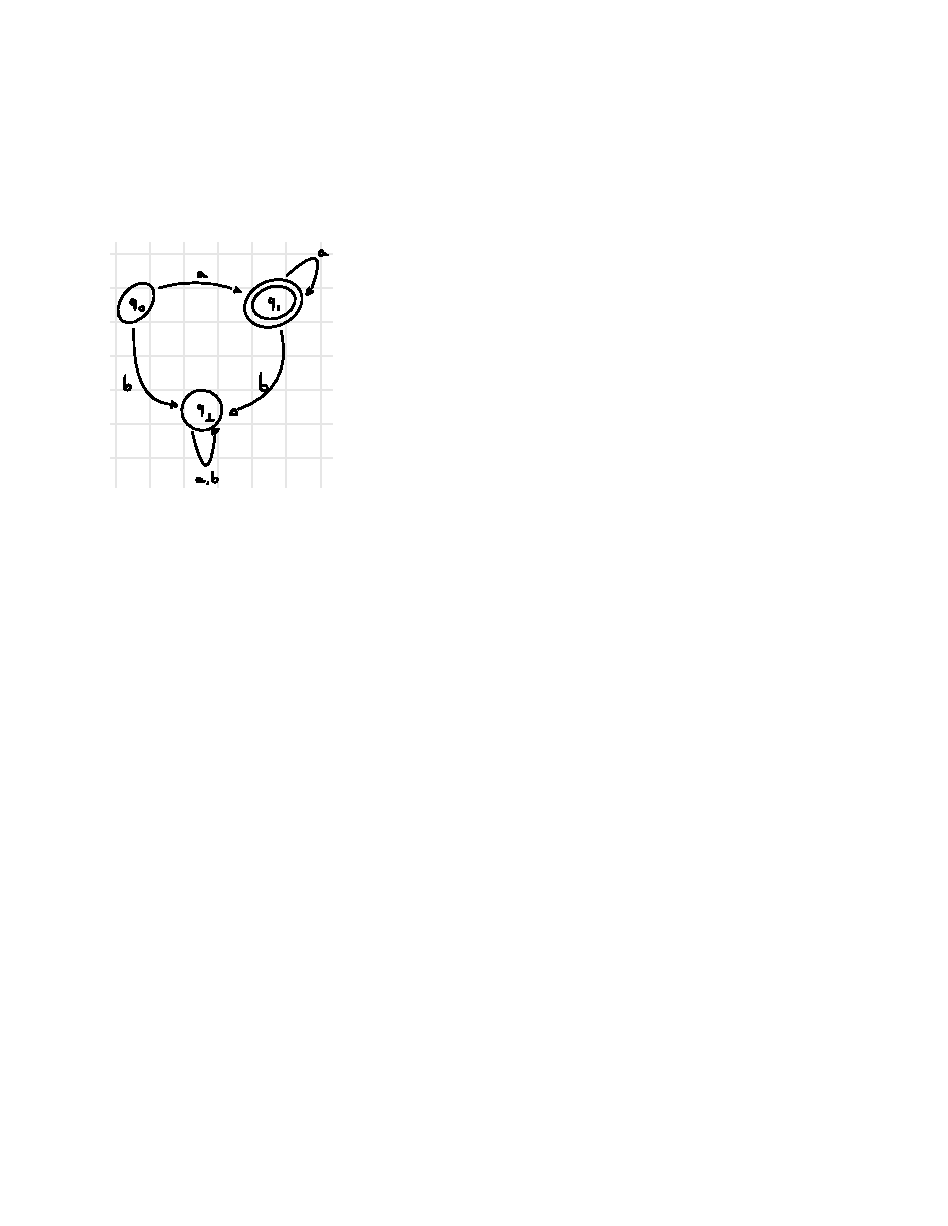
\includegraphics[width=0.5\textwidth]{img/esercitazioni/03_exe1.pdf}
			\caption{Grafo del linguaggio parametrizzato con il valore $0$.}
		\end{figure}
	
		\noindent
		Si esegue la dimostrazione del linguaggio regolare.
		
		\newpage
		
		\begin{proof}[\textbf{Dimostrazione $L\left(0\right)$}]
			Si dimostra tramite induzione.\newline
			
			\noindent
			\textbf{\underline{Caso base.}}\newline
			
			\begin{itemize}[label=-]
				\item $\begin{array}{lllll}
					x = \varepsilon & \notin L\left(0\right) & \hspace{1em} & \delta\left(q_{0}, \varepsilon\right) = q_{0} \notin F
				\end{array}$
				
				\item $\begin{array}{lllll}
					x = a & \in L\left(0\right) & \hspace{1em} & \delta\left(q_{0}, a\right) = q_{1} \in F
				\end{array}$
				
				\item $\begin{array}{lllll}
					x = b & \notin L\left(0\right) & \hspace{1em} & \delta\left(q_{0}, b\right) = q_{\bot} \notin F
				\end{array}$
			\end{itemize}
		
			\noindent
			\textbf{\underline{Passo induttivo.}}\newline
		
			\noindent
			Si dimostra per induzione che:
			
			\begin{equation*}
				\sigma \in L\left(0\right) \Longrightarrow \delta\left(q_{0}, \sigma\right) \in F
			\end{equation*}
		
			\noindent
			Supponendo che sia vero che la lunghezza della stringa $x$ sia minore di $n$, cioè $|x| < n$, allora:
			
			\begin{equation*}
				x \in L\left(0\right) \Longrightarrow \delta\left(q_{0}, x\right) \in F
			\end{equation*}
		
			\noindent
			A $x$ si assegna $a^{+}$, \textbf{N.B.}\footnote{Il segno del più indica un numero di concatenazione che è maggiore di zero ($a^{+} = a^{n}$, con $n > 0$). Al contrario, $a^{*} = a^{n}$ con $n \ge 0$.}, la $a^{+}$:
			
			\begin{itemize}[label=-]
				\item $x^{'} = xa \in L \hspace{2em} \delta\left(q_{0}, xa\right) = \delta\left(q_{1}, a\right) = q_{1} \in F$
				
				\item $x^{'} = xb \notin L \hspace{2em} \delta\left(q_{0}, xb\right) = \delta\left(q_{1}, b\right) = q_{\bot} \notin F$
			\end{itemize}
		
			\noindent
			Invece, adesso si dimostra il contrario:
			
			\begin{equation*}
				\sigma \notin L\left(0\right) \Longrightarrow \delta\left(q_{0}, \sigma\right) \notin F
			\end{equation*}
		
			\noindent
			Supponendo che sia vero che la lunghezza della stringa $x$ sia minore di $n$, cioè $|x| < n$, allora:
			
			\begin{equation*}
				x \notin L\left(0\right) \Longrightarrow \delta\left(q_{0}, x\right) \notin F
			\end{equation*}
		
			\noindent
			Si prende in considerazione il caso in cui la $x$ è:
			
			\begin{equation*}
				x = a^{*} \: b \: \left\{a,b\right\}^{*}
			\end{equation*}
			
			\noindent
			E si conclude la dimostrazione:
			
			\begin{itemize}[label=-]
				\item $x^{'} = xa \notin L\left(0\right) \hspace{2em} \delta\left(q_{0}, xa\right) = \delta\left(q_{\bot}, a\right) = q_{\bot} \notin F$
				
				\item $x^{'} = xb \notin L\left(0\right) \hspace{2em} \delta\left(q_{0}, xb\right) = \delta\left(q_{\bot}, a\right) = q_{\bot} \notin F$
			\end{itemize}
		\end{proof}
	
		\newpage
		
		\noindent
		Adesso, con il linguaggio parametrizzato si sostituisce il valore $1$:
		
		\begin{equation*}
			L\left(1\right) = \left\{a^{n} \: b \: a^{k} \: \left| \: n > 0, k \ge 0 \right.\right\}
		\end{equation*}
	
		\noindent
		L'automa a stati finiti deterministico è il seguente. La dimostrazione di questo linguaggio regolare si salta solamente per evidenziare la diversificazione con altri esercizi.
		
		\begin{figure}[!htp]
			\centering
			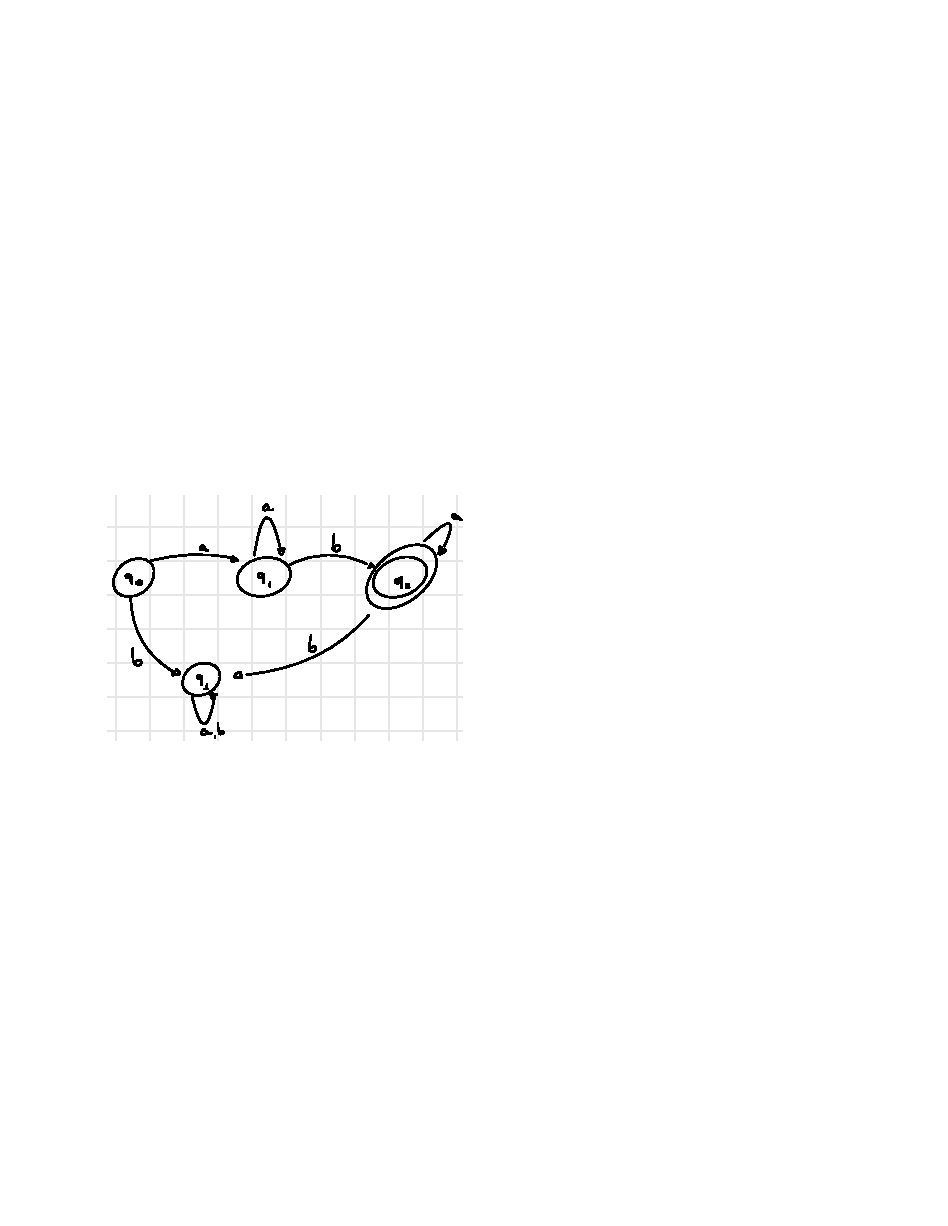
\includegraphics[width=0.5\textwidth]{img/esercitazioni/03_exe2.pdf}
			\caption{Automa a stati finiti deterministico del linguaggio parametrizzato con il valore $1$.}
		\end{figure}

		\noindent
		Si provano altri due, tre valori per verificare se il linguaggio continua ad essere regolare oppure no:
		
		\begin{itemize}
			\item $L\left(2\right) = \left\{a^{n} \: bb \: a^{k} \: \left| \: n = 2\mathbb{N} + 1, k \ge 0 \right.\right\}$
			\item $L\left(3\right) = \left\{a^{n} \: bbb \: a^{k} \: \left| \: n = 3\mathbb{N} + 1, k \ge 0 \right.\right\}$
			\item $L\left(4\right) = \left\{a^{n} \: bbbb \: a^{k} \: \left| \: n = 4\mathbb{N} + 1, k \ge 0 \right.\right\}$
		\end{itemize}
	
		\noindent
		Nonostante siano stati provati $3$ valori diversi, il linguaggio rimane regolare. Dunque, la dimostrazione si conclude dicendo che è stato \textbf{trovato un punto fisso}, ovvero il linguaggio è sempre regolare.
	\end{proof}

	\newpage
	
	\begin{proof}[\textbf{Dimostrazione $L\left(0\right)$}]
		Si dimostra la seguente unione:
		
		\begin{equation*}
			M = \bigcup_{m\in\mathbb{N}} L\left(m\right) = \left\{a^{n} \: b^{m} \: a^{k} \: \left| \: n \in m\mathbb{N} + 1, k \ge 0, m \ge 0 \right.\right\}
		\end{equation*}
	
		\noindent
		Si dimostra tramite il pumping lemma che per qualsiasi $h$ esiste una stringa $z$ tale per cui:
		
		\begin{equation*}
			\forall h \hspace{2em} \exists z = a^{h + 2} \: b^{h + 1}
		\end{equation*}
	
		\noindent
		Il pumping lemma, per definizione, afferma che $z = uvw$, che $|uv| \le h$ e infine che $|v| > 0$. Supponendo che $m = h + 1$, che $k = 0$ e che:
		
		\begin{equation*}
			n = h + 2 \in \left(h + 1\right) \mathbb{N} + 1 = 
			\begin{cases}
				1 \\
				h + 1 + 1 = h + 2 \xleftarrow{\text{elemento scelto per la dimostrazione}} \\
				2\left(h + 1\right) + 1 = 2h + 3 \\
				\cdots
			\end{cases}
		\end{equation*}
	
		\noindent
		L'obbiettivo è dimostrare che \dquotes{pompando} non si arriva né all'elemento precedente ($1$), né all'elemento successivo ($2\left(h + 1\right) + 1 = 2h + 3$). Si sceglie la classica stringa $z^{'}$:
		
		\begin{equation*}
			z^{'} = u v^{i} w = a^{h + 2 +\left(i - 1\right) |v|}  \: b^{h + 1} \hspace{2em} \text{con il vincolo } 0 < |v| \le h
 		\end{equation*}
	
		\noindent
		Si sceglie una $i$ per concludere la dimostrazione, in questo caso uguale a $2$:
		
		\begin{equation*}
			z^{'} = a^{h + 2 + |v|} \: b^{h + 1} \hspace{2em} \text{con il vincolo } |v| \le h 
		\end{equation*}
		
		\noindent
		Quindi l'intervallo in cui ricade la $|v|$ è:
		
		\begin{equation*}
			h + 2 < h + 2 + |v| \le 2h + 2 < 2h + 3 \xRightarrow{\text{si deduce}} z^{'} \notin L
		\end{equation*}
	
		\noindent
		\fcolorbox{Green4}{white}{%
			\parbox{\textwidth}{%
				\textcolor{Green4}{\textbf{Soluzione alternativa: uguaglianza tra esponenti.}}
				
				Esiste una alternativa, ovvero l'utilizzo dell'uguaglianza tra esponenti per dimostrare la negazione del pumping lemma. Per farla si prende in considerazione la stringa corrispondente alla $|v|$:
				
				\begin{equation*}
					\begin{array}{llllllll}
						&& h + 2	 	& \rightarrow	& \cancel{h + 2} = \cancel{h + 2} + |v|	& \rightarrow	& |v| = 0	& \textcolor{Green3}{\textbf{\checkmark}} \\
						& \nearrow &&&&&& \\
						h + 2 + |v| = &&&&&&& \\
						& \searrow &&&&&& \\
						&& 2h + 3	& \rightarrow 	& 2h + 3 = h + 2 + |v|				   	& \rightarrow	& |v| = h + 1	& \textcolor{Green3}{\textbf{\checkmark}}
					\end{array}
				\end{equation*}
				
				La prima espressione è dimostrata poiché chiaramente $|v| = 0$ non rispetta la definizione del pumping lemma. Anche la seconda è dimostrata perché $|v|$ al massimo può essere $h$ non $h + 1$.
			}
		}
		\:\newline
	\end{proof}

	\newpage
	
	\noindent
	\textcolor{Red3}{\textbf{\underline{Esercizio 9}}}\newline
	
	\noindent
	I dati dell'esercizio sono i seguenti:
	
	\begin{equation*}
		L = \left\{ 0^{k^{2}} \right\}
	\end{equation*}\newline
	
	\noindent
	L'esercizio riguarda un linguaggio e bisogna capire se è regolare oppure no.\newline
	
	\noindent
	\textcolor{Green4}{\textbf{\emph{Risoluzione.}}}\newline
	
	\noindent
	Il linguaggio non è regolare e si capisce dal fatto che non è possibile costruire una macchina che concateni una serie di $0$ per $k$ volte alla seconda.
	
	\begin{proof}[\textcolor{Blue3}{\textbf{Dimostrazione}}]
		Per ogni $n$ prendendo la stringa $z$:
		
		\begin{equation*}
			\forall n : z = 0^{n^{2}}
		\end{equation*}
	
		\noindent
		Il pumping lemma assicura che $z = uvw$, che $|uv| \le n$ e che $|v| < 0$. Si costruisce la stringa $z^{'}$:
		
		\begin{equation}
			z^{'} = 0^{n^{2} + |v| \left(i - 1\right)}
		\end{equation}
	
		Scegliendo una $i$ arbitraria, in questo caso $0$. Si esegue la dimostrazione tramite uguaglianza degli esponenti e disuguaglianza.\newline
		
		\noindent
		\textbf{\underline{Uguaglianza.}}
		
		\begin{equation*}
			\begin{array}{llllllllll}
				&& \cancel{n^{2}} - |v| = n^{2}			& \rightarrow	& |v| = 0											& \textcolor{Green3}{\textbf{\checkmark}} &&&& \\
				& \nearrow &&&&&&&& \\
				n^{2} - |v| &&&&&&&&& \\
				& \searrow &&&&&&&& \\
				&& n^{2} - |v| = \left(n - 1\right)^{2}	& \rightarrow 	& \cancel{n^{2}} - |v| = \cancel{n^{2}} - 2n + 1	& \rightarrow	&&&& \\
				&& |v| = 2n - 1	& \rightarrow & |v| \le n < 2n < -1	& \textcolor{Green3}{\textbf{\checkmark}} &&&&
			\end{array}
		\end{equation*}
	
		\noindent
		\textbf{\underline{Disuguaglianza.}}
		
		\begin{equation*}
			n ^{2} - n < n^{2} - |v| < n^{2}
		\end{equation*}
	\end{proof}

	\newpage
	
	\section{Linguaggi liberi dal contesto}
	
	\begin{center}
		\large
		\textbf{\emph{Introduzione}}
	\end{center}
	
	Una grammatica è un insieme di regole che permettono di generare un linguaggio. La situazione è quindi diversa rispetto ai linguaggi regolari. Infatti, quest'ultimi sono stati definiti come linguaggi \emph{riconosciuti} da una particolare famiglia di automi, i linguaggi in questo capitolo saranno \emph{generati} da particolari insiemi di regole. Un ruolo fondamentale in questo contesto è giocato dalle grammatiche libere dal contesto (CF) mediante le quali viene solitamente descritta la sintassi dei linguaggi di programmazione. Dunque, si vedrà come questi linguaggi siano anche riconosciuti da particolari automi, detti \emph{automi a pila}.
	
	\subsection{Linguaggi liberi dal contesto}
	
	Fino ad ora sono stati studiati i linguaggi regolari, i quali hanno visto la loro realizzazione pratica tramite gli automi. Un linguaggio, inoltre, veniva inizialmente studiato per capire se fosse regolare o no. Successivamente, si è rispettivamente eseguita la dimostrazione tramite automa (e matematica) per i primi e la negazione del Pumping Lemma per i secondi.
	
	Si è dunque vista la necessità di introdurre un mezzo per manipolare i linguaggi non regolari. Un primo strumento che viene introdotto è la \textcolor{Red3}{\textbf{\underline{grammatica}}} \textcolor{Red3}{\textbf{\underline{libera dal contesto}}} (CF, \emph{context free}), una quadrupla $G = \left\lbrace V, T, P, S \right\rbrace$ in cui:
	
	\begin{itemize}
	 	\item $V$, è un insieme finito di \textbf{\underline{variabili}} (chiamati anche \emph{\textbf{simboli non terminali}});
	 	
	 	\item $T$, è un insieme finito di \textbf{\underline{simboli terminali}} ($V \cap T = \emptyset$). È possibile vedere l'analogia con il $\Sigma$;
	 	
	 	\item $P$, è un insieme finito di \textbf{\underline{produzioni}} e indica le regole grammaticali. Ogni produzione è della forma $A \rightarrow \alpha$ in cui:
	 	\begin{itemize}
	 		\item $A \in V$ è una variabile;
	 		\item $\alpha \in \left(V \cup T\right)^{*}$.
	 	\end{itemize}
	 	
	 	\item $S \in V$, è una variabile speciale chiamata \textbf{\underline{simbolo iniziale}}.
	\end{itemize}

	\newpage

	\begin{center}
		\large
		\noindent
		\textcolor{Green4}{\textbf{\underline{Esempi concettuali}}}
	\end{center}

	\noindent
	\textcolor{Green4}{\textbf{\emph{Esempio 1}}}
	
	\noindent
	Si mostra un esempio introduttivo al concetto di linguaggi liberi dal contesto. Dato il seguente linguaggio:
	
	\begin{equation*}
		L = \left\{a^{n} \: b^{n} \: \left| \: n \ge 1 \right.\right\}
	\end{equation*}

	\noindent
	Si ha il seguente caso base:
	
	\begin{equation*}
		S \longrightarrow ab
	\end{equation*}

	\noindent
	In cui $S$ è sinonimo di $L$. Per dimostrarlo, si usa il passo induttivo:
	
	\begin{equation*}
		S \longrightarrow a \: \underbrace{a^{n} \: b^{n}}_{S} \: b \xrightarrow{\text{quindi...}} S \longrightarrow a \: S \: b
	\end{equation*}

	\noindent
	Attenzione! L'ordine è importante, infatti se viene sostituita la $S$, la stringa rimane regolare e dunque nel linguaggio. Per esempio, in questo modo è \emph{errato}:
	
	\begin{equation*}
		S \longrightarrow a \: b \: S \hspace{1em} \textcolor{Red3}{\text{NO!}}
	\end{equation*}
	\:\newline
	
	\noindent
	\textcolor{Green4}{\textbf{\emph{Esempio 2}}}
	
	\noindent
	Dato il seguente linguaggio:
	
	\begin{equation*}
		L = \left\{a^{2n} \: b^{2n} \: \left| \: n \ge 0 \right.\right\}
	\end{equation*}

	\noindent
	Il simbolo iniziale è la $\varepsilon$ e doppia $a$, doppia $b$:
	
	\begin{equation*}
		\begin{array}{lll}
			S & \longrightarrow & \varepsilon \\
			S & \longrightarrow & a \: a \: S \: b \: b
		\end{array}
	\end{equation*}
	\:\newline
	
	\noindent
	\fcolorbox{black}{white}{%
		\parbox{\textwidth}{%
			\textcolor{Red3}{\textbf{Linguaggi generati.}}
			
			Più in generale, il \textcolor{Red3}{\textbf{linguaggio generato da} $G$} è definito come:
			
			\begin{equation*}
				L\left(G\right) = \left\{w \in T^{*} \: \left| \: S \overset{G}{\Longrightarrow}_{*} w \right.\right\}
			\end{equation*}
		
			La freccia $\overset{G}{\Longrightarrow}_{*}$ indica una \textbf{derivazione finita}, ovvero con una serie \underline{finita} di passi si arriva a $w$.\newline
		
			Inoltre, $L$ è un \textcolor{Red3}{\textbf{\underline{linguaggio libero dal contesto}}} (CF) se esiste una grammatica CF ($G$) tale che $L = L\left(G\right)$. Si osservi che due grammatiche $G_{1}$ e $G_{2}$ sono equivalenti se $L\left(G_{1}\right) = L\left(G_{2}\right)$
		}
	}

	\newpage
	
	\noindent
	\textcolor{Green4}{\textbf{\emph{Esempio 3}}}
	
	\noindent
	Il linguaggio è il seguente:
	
	\begin{equation*}
		L = \left\{a^{n} \: b^{n} \: \left| \: n \ge 0 \right.\right\}
	\end{equation*}

	\noindent
	Si ottiene la grammatica del linguaggio:
	
	\begin{equation*}
		\begin{array}{lll}
			S & \longrightarrow & \varepsilon \\
			S & \longrightarrow & a \: S \: b
		\end{array}
	\end{equation*}
	
	\noindent
	L'obbiettivo è dimostrare che il linguaggio sia $L \subseteq L\left(G\right)$, sia $L = L\left(G\right)$ e infine $L \supseteq L\left(G\right)$.
	
	\begin{proof}[\textcolor{Blue3}{\textbf{Dimostrazione caso} $L \subseteq L\left(G\right)$}]
		Si definisce il caso base con $n = 0$:
		
		\begin{equation*}
			n = 0 \xrightarrow{\text{sostituzione nella stringa}} a^{0} \: b^{0} = \varepsilon
		\end{equation*}
	
		\noindent
		Grazie alla prima regola l'affermazione è vera, dunque l'ipotesi induttiva è:
		
		\begin{equation*}
			n \ge 0 \hspace{2em} a^{n} \: b^{n} \Longrightarrow S \longrightarrow_{*} a^{n} \: b^{n}
		\end{equation*}
	
		\noindent
		E l'induzione è la seguente:
		
		\begin{equation*}
			a^{n+1} \: b^{n+1} = a \: \underbrace{a^{n} \: b^{n}}_{S} \: b \Longrightarrow S \rightarrow a \: S \: b \rightarrow a \: a^{n} \: b^{n} \: b = a^{n+1} \: b^{n+1} \hspace{1em} \textcolor{Green4}{\textbf{\checkmark}}
		\end{equation*}
	\end{proof}

	\begin{proof}[\textcolor{Blue3}{\textbf{Dimostrazione caso} $L\left(G\right) \supseteq L$}]
		Si definisce il caso base con $n = 1$:
		
		\begin{equation*}
			n = 1 \xrightarrow{\text{la grammatica è}} S \rightarrow \varepsilon \hspace{1em} \text{con } \varepsilon \in L
		\end{equation*}
		
		\noindent
		L'ipotesi induttiva è:
		
		\begin{equation*}
			n \ge 1 \hspace{2em} \forall m \le n : S \longrightarrow_{m} x \Longrightarrow x = a^{k} \: b^{k} \in L \hspace{2em} \text{con } x \in T^{*}
		\end{equation*}
		
		\noindent
		E l'induzione è la seguente:
		
		\begin{equation*}
			\underbrace{S \longrightarrow a \: S \: b \longrightarrow_{*} a \: x \: b}_{m + 1} \xrightarrow{\text{sostituzione } x} a^{k+1} \: b^{k+1} \in L \hspace{1em} \textcolor{Green4}{\textbf{\checkmark}}
		\end{equation*}
	\end{proof}

	\newpage
	
	\noindent
	\textcolor{Green4}{\textbf{\emph{Esempio 4}}}
	
	\noindent
	Il linguaggio è il seguente:
	
	\begin{equation*}
		L = \left\{a^{n} \: b^{h} \: c^{h} \: d^{n} \: \left| n, h \ge 0 \right.\right\}
	\end{equation*}

	\noindent
	La grammatica generata non è con $\varepsilon$, invece è:
	
	\begin{equation*}
		\begin{array}{llll}
			\cancel{S} & \longrightarrow & \cancel{\varepsilon} & \textcolor{Red3}{\textbf{No}} \\
			S & \longrightarrow & a \: S \: d & \textcolor{Green4}{\textbf{Sì}}
		\end{array}
	\end{equation*}

	\noindent
	Per includere anche $b$ e $c$ si deve specificare:
	
	\begin{equation*}
		\begin{array}{lll}
			S & \longrightarrow & a \: S \: d \: |H \\
			H & \longrightarrow & b \: H \: c \: |\varepsilon \\
		\end{array}
	\end{equation*}
	
	\noindent
	La grammatica ha $H$ che può essere anche $\varepsilon$ perché la variabile $h$ può essere zero.\newline
	
	\noindent
	\textcolor{Green4}{\textbf{\emph{Esempio 5}}}
	
	\noindent
	Dato il seguente linguaggio:
	
	\begin{equation*}
		L = \left\{a^{n} \: b^{n} \: c^{h} \: \left| \: n,h \ge 0\right.\right\}
	\end{equation*}

	\noindent
	In cui si raggruppa la stringa in due acronimi:
	
	\begin{equation*}
		\begin{array}{lll}
			A & = & a^{n} \: b^{n} \\
			C & = & c^{h}
		\end{array}
	\end{equation*}

	\noindent
	Quindi, la grammatica relativa è:
	
	\begin{equation*}
		\begin{array}{lll}
			S & \longrightarrow & A \: C \\
			A & \longrightarrow & a \: A \: b \: | \varepsilon \\
			C & \longrightarrow & c \: C | \varepsilon
		\end{array}
	\end{equation*}
	\:\newline
	
	\noindent
	\textcolor{Green4}{\textbf{\emph{Esempio 6}}}
	
	\noindent
	Dato il seguente linguaggio:
	
	\begin{equation*}
		L = \left\{a^{n} \: c^{m} \: b^{n} \: \left| \: n,m \ge 0\right.\right\}
	\end{equation*}

	\noindent
	La grammatica che genera il linguaggio è:
	
	\begin{equation*}
		\begin{array}{lll}
			S & \longrightarrow & a \: S \: b \: | c \\
			S & \longrightarrow & c \: C \: | \varepsilon
		\end{array}
	\end{equation*}
	
	\newpage
	
	\noindent
	\textcolor{Green4}{\textbf{\emph{Esempio 7}}}
	
	\noindent
	Dato il seguente linguaggio:
	
	\begin{equation*}
		L = \left\{0^{n} \: 1^{m} \: 0^{n + m} \: | \: n,m \ge 0\right\}
	\end{equation*}

	\noindent
	Il linguaggio può essere scomposto come:
	
	\begin{equation*}
		L = \left\{0^{n} \: 1^{m} \: 0^{m} \: 0^{n} \: | \: n,m \ge 0\right\}
	\end{equation*}

	\noindent
	La grammatica che genera il linguaggio è:
	
	\begin{equation*}
		\begin{array}{lll}
			S & \longrightarrow & 0 \: S \: 0 \: | A \\
			A & \longrightarrow & 1 \: A \: 0 \: | \varepsilon
		\end{array}
	\end{equation*}
	\:\newline
	
	\noindent
	\textcolor{Green4}{\textbf{\emph{Esempio 8}}}
	
	\noindent
	Dato il seguente linguaggio:
	\begin{equation*}
		L = \left\{\sigma \in \left\{0,1\right\}^{*} \: \left| \: \sigma \text{ è polindroma} \right.\right\}
	\end{equation*}

	\noindent
	La grammatica che genera il linguaggio è:
	\begin{equation*}
		\begin{array}{lll}
			S & \longrightarrow & 0 \: | \: 1 \: | \: \varepsilon \\
			S & \longrightarrow & 0 \: S \: 0 \: | \: 1 \: S \: 1
		\end{array}
	\end{equation*}
	\:\newline
	
	\noindent
	\textcolor{Green4}{\textbf{\emph{Esempio 9}}}
	
	\noindent
	Dato il seguente linguaggio:
	\begin{equation*}
		L = \left\{w \in \left\{a,b\right\}^{+} \: \left| \: |w|_{a} = |w|_{b} \right.\right\}
	\end{equation*}

	\noindent
	La grammatica che genera il linguaggio è:
	\begin{equation*}
		S \longrightarrow a \: b \: | \: b \: a \: | \: a \: S \: b \: | \: b \: S \: a \: | \: S \: S
	\end{equation*}\newpage
	
	\section{Funzioni parziali ricorsive di S.C. Kleene}
	
	\subsection{Funzioni primitive ricorsive}
	
	Una funzione ricorsiva è una funzione dove il suo valore per un dato argomento è direttamente correlato al valore della medesima funzione su argomenti \dquotes{più semplici} o al valore di funzioni \dquotes{più semplici}.\newline
	Per esempio, la funzione definisce ricorsivamente la successione di Fibonacci: $1, 1, 2, 3, 5, 8, 13, \cdots$
	\begin{equation*}
		\begin{array}{lll}
			f\left(0\right) 	& = & 1 \\
			f\left(1\right) 	& = & 1 \\
			f\left(x+2\right) 	& = & f\left(x+1\right) + f\left(x\right)
		\end{array}
	\end{equation*}
	Quindi, per \textcolor{Red3}{\textbf{funzioni ricorsive di base}} si intende le seguenti funzioni:
	\begin{itemize}
		\item La funzione \textbf{costante} $0: \lambda x. 0$;
		\item La funzione \textbf{successore} $S: \lambda x. x+1$;
		\item La funzione \textbf{identità}, o \emph{i}-esima proiezione, $\pi_{i}: \lambda x_{1} \cdots x_{n}. x_{1}$ con $1~\le~i~\le~n$.
	\end{itemize}
	Con la lettera greca lambda $\lambda$, si parla di funzione che ha come argomento la funzione accanto e restituisce il valore dopo il punto (\textbf{\emph{lambda notation}}). Per esempio, con l'espressione $\lambda x. 0$, si intende che la funzione lambda prende la funzione $x$ come argomento e restituisce il valore $0$ come output.\newline
	
	\noindent
	Inoltre, si definisce anche una funzione $f: \mathbb{N}^{n} \longrightarrow \mathbb{N}$ che viene definita:
	\begin{itemize}
		\item Per \textbf{composizione} da $g_{1}, \cdots, g_{k}: \mathbb{N}^{n} \longrightarrow \mathbb{N}$ e $h: \mathbb{N}^{k} \longrightarrow \mathbb{N}$ se:
		\begin{equation*}
			f\left(x_{1}, \cdots, x_{n}\right) = h\left(g_{1}\left(x_{1}, \cdots, x_{n}\right), \cdots, g_{k}\left(x_{1}, \cdots, x_{n}\right)\right)
		\end{equation*}
		
		\item Per \textbf{ricorsione primitiva} da $g:\mathbb{N}^{n-1} \longrightarrow \mathbb{N}$ e $h:\mathbb{N}^{n+1} \longrightarrow \mathbb{N}$ se:
		\begin{equation*}
			\begin{cases}
				f\left(x_{1}, \cdots, x_{n-1}, 0\right) = g\left(x_{1}, \cdots, x_{n-1}\right) \\
				f\left(x_{1}, \cdots, x_{n-1}, y+1\right) = h\left(x_{1}, \cdots, x_{n-1}, y, f\left(x_{1}, \cdots, x_{n-1}, y\right)\right)
			\end{cases}
		\end{equation*}
	\end{itemize}
	Tutte e solo le funzioni definibili a partire dalle precedenti funzioni ricorsive di base mediante composizione e ricorsione primitiva definiscono l'\textbf{insieme} delle \textcolor{Red3}{\textbf{funzioni primitive ricorsive}}. In altre parole, l'idea è costruire via via funzioni effettivamente calcolabili a partire dalle funzioni di base, come $0$, costruendo da queste, per composizione e ricorsione primitiva, funzioni via via più complesse.\newline
	
	\noindent
	Si definisce la \textbf{classe $\mathcal{P}$} come la \textbf{classe delle funzioni primitive ricorsive}. Essa corrisponde alla più piccola classe, ovvero l'intersezione di tutte le classi, di funzioni contenenti le funzioni ricorsive di base e chiuse per composizione e ricorsione primitiva.\newpage
	
	\begin{theorem}
		Le funzioni primitive ricorsive sono \textbf{totali}.
	\end{theorem}
	\noindent
	Questo teorema pone una limitazione sulle funzioni primitive ricorsive. Ovvero, l'insieme non ammette quelle funzioni calcolabili che possono essere indefinite su alcuni, o tutti, i valori di input. Le funzioni primitive ricorsive hanno inoltre un'ulteriore limitazione anche all'interno delle funzioni calcolabili e totali sui naturali. Per dimostrare questo fatto, si utilizza una funzione evidentemente calcolabile e totale, ma non appartenente a $\mathcal{P}$, ovvero la \textbf{funzione di Ackermann}:
	\begin{equation*}
		\begin{cases}
			\begin{array}{lll}
				\mathrm{ack}\left(0, y\right) 	& = & y+1 \\
				\mathrm{ack}\left(x+1, 0\right) & = & \mathrm{ack}\left(x+1\right) \\
				\mathrm{ack}\left(x+1, y+1\right) & = & \mathrm{ack}\left(x, \mathrm{ack}\left(x+1, y\right)\right)
			\end{array}
		\end{cases}
	\end{equation*}
	Alcuni esempi:
	\begin{equation*}
		\begin{array}{lll}
			\mathrm{ack}\left(0,y\right) & = & y+1 \\
			&& \\
			\mathrm{ack}\left(1,y\right) & = & 2+\left(y+3\right)-3 \\
			&& \\
			\mathrm{ack}\left(2,y\right) & = & 2\left(y+3\right)-3 \\
			&& \\
			\mathrm{ack}\left(3,y\right) & = & 2^{y+3} - 3 \\
			&& \\
			\mathrm{ack}\left(4,y\right) & = & 2^{\overbrace{{2^{.. 2}}}^{y+3}} - 3
		\end{array}
	\end{equation*}
	La funzione ack cresce più velocemente di qualunque funzione ricorsiva primitiva. Questa funzione, universalmente accettata come funzione calcolabile, non può essere quindi primitiva ricorsiva pur essendo totale.
	\begin{theorem}
		La funzione di Ackermann $\mathrm{ack}$ non è ricorsiva primitiva.
	\end{theorem}\newpage
	
	\subsection{Macchina di Turing}
	
	Indipendentemente dal problema che si intende risolvere, gli algoritmi hanno alcune caratteristiche comuni. Si elencano qui di seguito per comprendere meglio la macchina di Turing:
	\begin{enumerate}
		\item Un algoritmo è di lunghezza finita.
		
		\item Esiste un agente di calcolo che porta avanti il calcolo eseguendo le istruzioni dell'algoritmo.
		
		\item L'agente di calcolo ha a disposizione una memoria dove vengono immagazzinati i risultati intermedi del calcolo.
		
		\item Il calcolo avviene per passi discreti.
		
		\item Il calcolo non è probabilistico.
		
		\item Non deve esserci alcun limite finito alla lunghezza dei dati di ingresso.
		
		\item Non deve esserci alcun limite alla quantità di memoria disponibile.
		
		\item Sono ammesse esecuzioni con un numero di passi finito ma illimitato.
	\end{enumerate}
	I primi tre punti (1,2,3) sono ovvi.\newline
	Il punto 4 afferma che il calcolo non avviene mediante dispositivi analogici.\newline
	Il punto 5 afferma che il calcolo non obbedisce a nessuna legge di probabilità.\newline
	Il punto 6 è ragionevole poiché, per esempio, dato un algoritmo di somma, esso deve poter funzionare per ogni possibile addendo, ovvero qualsiasi numero naturale.\newline
	Il punto 7 si assume corretto poiché limitandola, alcuni algoritmi noti per calcolare semplici funzioni non potrebbero funzionare.\newline
	Il punto 8 afferma che non essendo limitabile il numero di passi richiesti per eseguire un generico algoritmo, allora non è possibile stabilire a priori un limite massimo sul numero di passi nell'esecuzione di un algoritmo.\newline
	
	\noindent
	L'idea di A.M. Turing fu quella di creare matematicamente la \textcolor{Red3}{\textbf{Macchina di Turing}} (MdT). L'idea è quella di pensare ad una semplice macchina in grado di scrivere simboli su un nastro potenzialmente infinito, rappresentando il fatto, anche espresso nel punto 7, che nei calcoli abbiamo a disposizione una quantità illimitata di carta dove registrare i risultati parziali del calcolo.\newline
	Il nastro è fatto di celle che rappresentano la quantità di memoria unitaria. La macchina utilizzerà un alfabeto finito, col quale possiamo rappresentare una infinità (numerabile) di dati. Il corpo pesante della macchina (detto controllo) sarà realizzato mediante un automa a stati finiti deterministico (DFA).
	
	Una MdT è quindi un dispositivo di calcolo rappresentabile con un nastro di lunghezza illimitata nel quale vengono immagazzinati i dati o sequenze di simboli del calcolo. Uno di questi simboli è \$ rappresentante l'assenza di simboli (spazio bianco). Il controllo MdT ha accesso al nastro attraverso una testina di lettura e scrittura che permette di leggere o scrivere un simbolo alla volta.\newline
	Ad ogni istante nel calcolo, il simbolo presente nella casella esaminata dalla testina rappresentata l'input alla macchina, in figura il simbolo $s$. In risposta la macchina può decidere di modificare il simbolo e/o spostare il nastro a sinistra o a destra della casella esaminata.
	\begin{figure}[!htp]
		\centering
		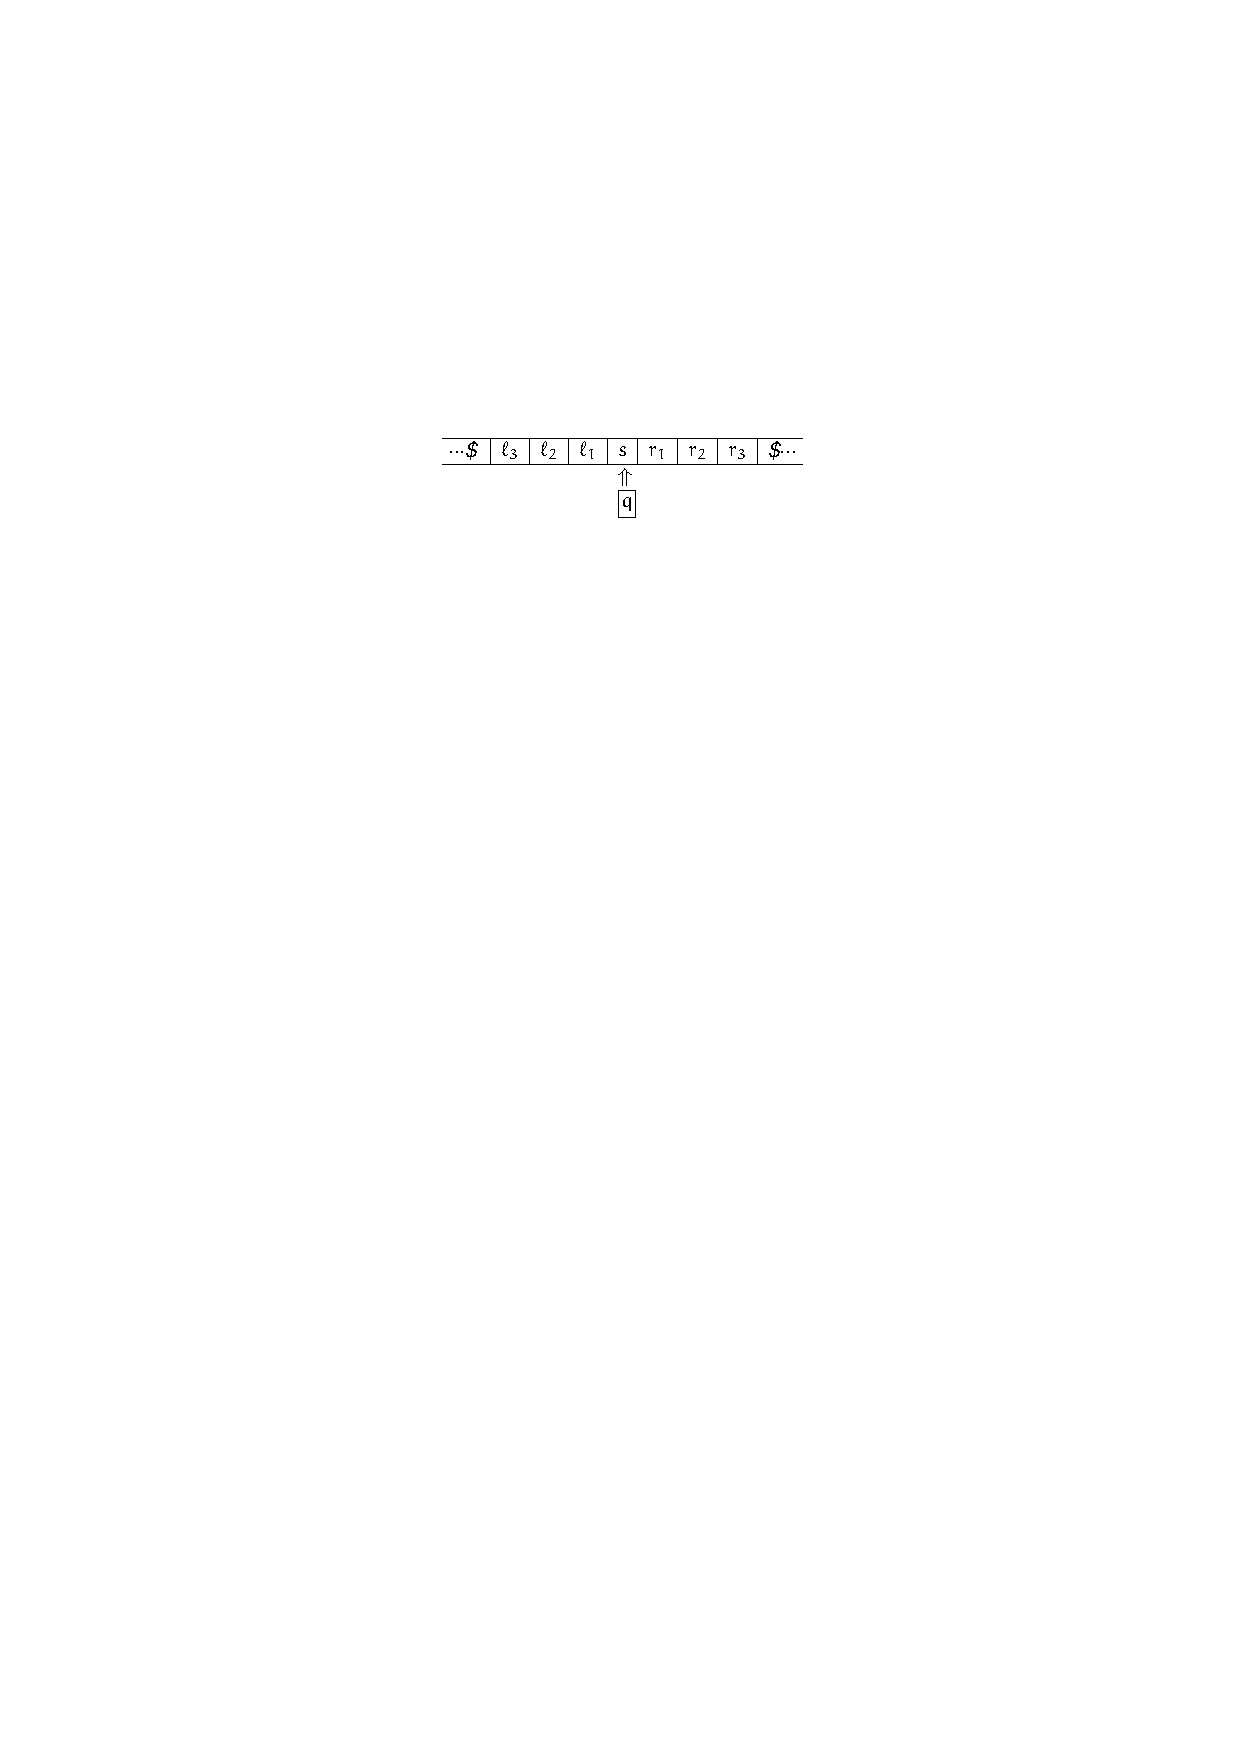
\includegraphics[width=.6\textwidth]{img/MdT.pdf}
		\caption{Il modello meccanico della Macchina di Turing.}
	\end{figure}

	\noindent
	\begin{theorem}
		Una \textcolor{Red3}{\textbf{descrizione istantanea}} (ID, Instant Description) di una MdT è una quadrupla:
		\begin{equation*}
			\left\langle q,v,s,w \right\rangle
		\end{equation*}
		dove $v,w \in \Sigma^{*}$ rappresentano i caratteri significativi (cioè escludendo la sequenza illimitata di \$ sempre presenti a desta e a sinistra) presenti sul nastro a sinistra ed a destra della testina, $s$ è il simbolo letto dalla testina, essendo la macchina nello stato $q$.
	\end{theorem}
	\noindent
	Ad esempio, nella MdT in figura, la ID corrispondente è $\left\langle q, l_{3}, l_{2}, l_{1}, s, r_{1}, r_{2}, r_{3} \right\rangle$.\newline
	
	\noindent
	Una MdT così descritta soddisfa pienamente i requisiti per la definizione ragionevole di algoritmo:
	\begin{enumerate}
		\item Le istruzioni della MdT sono finite.
		\item La MdT è l'agente di calcolo che esegue l'algoritmo.
		\item Il nastro rappresenta la memoria della macchina.
		\item La MdT opera in modo discreto.
		\item Ad ogni ID corrisponde una sola azione (determinismo della MdT).
		\item Non esiste alcun limite all'input, essendo il nastro illimitato.
		\item La capacità della memoria (nastro) è illimitata.
		\item Le operazioni eseguibili sono semplici e quindi di complessità limitata.
		\item Non esiste alcun limite al numero di istruzioni eseguite in quanto la medesima quintupla può essere usata più volte.
		\item Possono esistere MdT che non calcolano nulla generando una sequenza infinita di ID.
	\end{enumerate}
	Una funzione viene $f: \mathbb{N}^{n} \longrightarrow \mathbb{N}$ è \textcolor{Red3}{\textbf{Turing calcolabile}} se esiste una MdT M tale che, partendo dalla configurazione iniziale:
	\begin{equation*}
		\cdots \$\$\$ \underbrace{\$}_{q_{0}} \underline{x_{1}} \$ \cdots \$ \underline{x_{n}} \$\$\$\cdots
	\end{equation*}
	se $f\left(x_{1}, \cdots, x_{n}\right)$ è definita allora M termina nella configurazione:
	\begin{equation*}
		\cdots \$\$\$ \cdots \underbrace{\$}_{q_{f}} \underline{f\left(x_{1}, \cdots, x_{n}\right)} \$ \cdots
	\end{equation*}
	si assume che a sinistra e a destra dell'input nella configurazione iniziale ci siano solo \$.\newpage
	
	\subsection{Funzioni parziali ricorsive di S.C. Kleene}
	
	Esiste un metodo generale per costruire funzioni parziali a partire da funzioni totali, ad esempio le primitive ricorsive.\newline
	
	\noindent
	Sia $f$ una funzione \underline{totale} $n+1$ aria, allora si definisce la funzione:
	\begin{equation*}
		\begin{array}{lll}
			\varphi\left(x_{1}, \cdots, x_{n}\right) & = & \mu z. \left(f\left(x_{1}, \cdots, x_{n}, z\right) = 0\right) \\
			&& \\
			& = & \begin{cases}
				\text{il più piccolo } z: f\left(x_{1}, \cdots, x_{n}, z\right) = 0		& \text{se } z \text{ esiste} \\
				\uparrow																& \text{altrimenti}
			\end{cases}
		\end{array}
	\end{equation*}
	Tale operatore tra funzioni è detto $\mu$-operatore ed una funzione così definita è detta definita per minimizzazione o \textcolor{Red3}{$\boldsymbol{\mu}$\textbf{-ricorsione}} da $f$. Chiaramente una funzione definita per minimizzazione è in generale, per definizione, parziale. In altre parole, si cerca lo $z$ più piccolo che azzeri la funzione.\newline
	
	\noindent
	La classe delle funzioni \textcolor{Red3}{\textbf{parziali ricorsive}} è la minima classe $\mathcal{P}_{\mu}$ di funzioni contenente $\mathcal{P}$ e chiusa per $\mu$-ricorsione.\newline
	
	\noindent
	Il seguente risultato dimostra l'equivalenza delle funzioni calcolabili da MdT e le funzioni parziali ricorsive di S.C. Kleene $\mathcal{P}_{\mu}$.
	\begin{theorem}
		$\varphi \in \mathcal{P}_{\mu}$ se e solo se $\phi$ è Turing-calcolabile.
	\end{theorem}
	
	\noindent
	Si definisce la \textcolor{Red3}{\textbf{tesi di Church-Turing}} come la classe delle funzioni \dquotes{intuitivamente calcolabili} coincide con la classe delle funzioni Turing calcolabili.\newline
	\begin{theorem}
		Esiste un programma chiamato \textcolor{Red3}{\textbf{interprete}} tale che INT: $\mathbb{N} \times \mathbb{N}^{n} \rightarrow \mathbb{N}$:
		\begin{equation*}
			\varphi_{int}\left(x,y\right) = \begin{cases}
				\varphi_{x}\left(y\right)	& \text{se } \varphi_{x}\left(y\right)\downarrow \\
				\uparrow					& \text{altrimenti}
			\end{cases}
		\end{equation*}
	\end{theorem}\newpage

	\subsection{Il teorema s-m-n}
	
	Il \textcolor{Red3}{\textbf{teorema s-m-n}} è dovuto a S.C. Kleene ed è fondamentale. Anch'esso rappresenta un esempio di dimostrazione basata sulla Tesi di Church-Turing.
	\begin{theorem}[\textbf{s-m-n}]
		Per ogni coppia di interi $m,n \ge 1$ esiste una funzione ricorsiva totale $s_{n}^{m}$ di $m+1$ variabili tale che per ogni $x, y_{1}, \cdots, y_{m}$ si ha che:
		\begin{equation*}
			\forall z_{1} \cdots z_{n}. \varphi_{x}\left(y_{1}, \cdots, y_{m}, z_{1}, \cdots, z_{n}\right) = \varphi_{s_{n}^{m}\left(x,y_{1}, \cdots, y_{m}\right)} \left(z_{1}, \cdots, z_{n}\right)
		\end{equation*}
	\end{theorem}
	\noindent
	Il teorema s-m-n gioca un ruolo essenziale nello sviluppo della teoria della ricorsività. Il significato è più o meno il seguente: se avete scritto un programma che implementa un certo algoritmo su $m+n$ dati in input e da un certo momento in poi $m$ di questi sono fissati, allora sapete ottenere un programma \dquotes{\textbf{specializzato}} che accetta solo $n$ parametri in input e che calcola la stessa funzione per questi $n$ parametri.
	\begin{theorem}
		Esiste una funzione ricorsiva $g$ in due argomenti tale che per ogni $x$ e $y$: $\varphi_{g\left(x,y\right)} = \varphi_{x} \circ \varphi_{y}$
	\end{theorem}

	\longline

	\subsection{Problemi insolubili}
	
	Esistono molti problemi insolubili, ma uno dei più classici è il \textcolor{Red3}{\textbf{problema della terminazione}} posto da Turing: esiste una procedura effettiva tale che dati $x$ e $y$ determina se $\varphi_{x}\left(y\right)$ è definita o no?\newline
	
	\noindent
	Più formalmente, non esiste una funzione ricorsiva $g$ tale che per ogni $x$:
	\begin{equation*}
		g\left(x\right) = \begin{cases}
			1 & \text{se } \varphi_{x}\left(x\right) \downarrow \\
			0 & \text{se } \varphi_{x}\left(x\right) \uparrow
		\end{cases}
	\end{equation*}
	\begin{theorem}
		Non esiste una funzione ricorsiva $\varphi$ tale che per ogni $x$ e $y$:
		\begin{equation*}
			\varphi\left(x,y\right) = \begin{cases}
				1 & \text{se } \varphi_{x}\left(y\right) \downarrow \\
				0 & \text{se } \varphi_{x}\left(y\right) \uparrow
			\end{cases}
		\end{equation*}
	\end{theorem}
	\noindent
	Non esiste una funzione ricorsiva $f$ tale che per ogni $x$:
	\begin{equation*}
		f\left(x\right) = \begin{cases}
			1 & \text{se } \varphi_{x} \text{ è totale} \\
			0 & \text{se } \varphi_{x} \text{ non è totale}
		\end{cases}
	\end{equation*}\newpage
	
	\section{Insiemi ricorsivi e ricorsivamente enumerabili}
	
	\subsection{Insiemi ricorsivi e ricorsivamente enumerabili}
	
	Un insieme $I \subseteq \mathbb{N}$ è detto \textcolor{Red3}{\textbf{ricorsivamente enumerabile}} (r.e.) se esiste una funzione ricorsiva (parziale o totale) $\varphi$ tale che $I = \mathrm{dom}\left(\varphi\right)$.\newline
	
	\noindent
	Inoltre, nel seguito indicheremo con:
	\begin{itemize}
		\item $W_{x}$ l'insieme r.e. associato al dominio della funzione $\varphi_{x}$:
		\begin{equation*}
			W_{x} = \mathrm{dom}\left(\varphi_{x}\right) = \left\{y \: | \: \varphi_{x}\left(y\right) \downarrow\right\}
		\end{equation*}
		essendo $\varphi_{x}$ l'$x$-esima MdT nella numerazione fissata.
		
		\item $\mathrm{range}_{x}$ l'insieme $\mathrm{range}_{x} = \left\{y \: | \: \exists z \varphi_{x}\left(z\right)\downarrow \land \varphi_{x}\left(z\right) = y\right\}$ ovvero il codominio della funzione parziale ricorsiva $\varphi_{x}$.
	\end{itemize}
	Sia $A \in RE$. La funzione parziale:
	\begin{equation*}
		\varphi_{A}\left(x\right) = \begin{cases}
			1			& \text{se } x \in A \\
			\uparrow	& \text{se } x \notin A
		\end{cases}
	\end{equation*}
	è detta \textbf{funzione semicaratteristica} dell'insieme $A$. È chiaro che $A = \mathrm{dom}\left(\varphi_{A}\right)$.\newline
	
	\noindent
	Un insieme $I \subseteq \mathbb{N}$ è detto \textcolor{Red3}{\textbf{ricorsivo}} (REC) se esiste una funzione ricorsiva (totale) $f_{1}$ tale che:
	\begin{equation*}
		f_{1}\left(x\right) = \begin{cases}
			1 & \text{se } x \in I \\
			0 & \text{se } x \notin I
		\end{cases}
	\end{equation*}
	I seguenti esempi sono insiemi ricorsivi:
	\begin{itemize}
		\item L'insieme $\left\{0,2,4,6,...\right\}$ dei numeri pari;
		\item $\mathbb{N}$ e $\emptyset$;
		\item Ogni insieme finito;
		\item Ogni insieme $A$ tale che $\overline{A}$ è finito.
	\end{itemize}
	Dato $A$ insieme ricorsivo, si definisce la funzione parziale e chiaramente ricorsiva:
	\begin{equation*}
		\varphi\left(x\right) = \begin{cases}
			1 & \text{se } f_{A}\left(x\right) = 1 \\
			\uparrow & \text{altrimenti}
		\end{cases}
	\end{equation*}
	Se un \textbf{insieme è ricorsivo allora è anche ricorsivamente enumerabile}:
	\begin{equation*}
		A \in \mathrm{REC} \Longrightarrow A \in \mathrm{r.e.}
	\end{equation*}
	\begin{theorem}[\textbf{Teorema di Post}]
		Un insieme $A$ è ricorsivo se e solo se $A$ e $\overline{A}$ sono r.e.
		\begin{equation*}
			A \in \mathrm{REC} \iff A, \overline{A} \in \mathrm{r.e.}
		\end{equation*}
	\end{theorem}
	\noindent
	Si definisce \textbf{la funzione} $K = \left\{x \: | \: \varphi_{x}\left(x\right) \downarrow\right\}$. È chiaro per la definizione che $K = \left\{x \: | \: x \in W_{x}\right\}$.
	\begin{theorem}
		K è r.e. ma non ricorsivo.
	\end{theorem}

	\noindent
	Esiste una \textcolor{Red3}{\textbf{caratterizzazione degli insiemi}} r.e. per cui le seguenti affermazioni sono equivalenti:
	\begin{itemize}
		\item $A \in \mathrm{RE}$;
		\item $A = \mathrm{range}\left(\varphi_{p}\right)$ con $p$ parziale ricorsiva;
		\item $A = \emptyset$ oppure $A = \mathrm{range}\left(\varphi_{p}\right)$ con $p$ totale ricorsiva.
	\end{itemize}
	\begin{theorem}
		Si afferma che: $A \in \mathrm{REC} \iff A=\emptyset$ oppure $A = \mathrm{range}\left(f_{P}\right)$ con $f_{P}$ totale ricorsiva non decrescente.
	\end{theorem}
	\begin{theorem}
		$A \in \mathrm{REC},\left|A\right| = W \iff A = \mathrm{range}\left(f\right)$ con $f$, allora è \textcolor{Red3}{\textbf{totale ricorsiva crescente}}.
	\end{theorem}
	\begin{theorem}
		$A$ è r.e. e $\left|A\right| = W \Longrightarrow \exists B \in \mathrm{REC}$ tale che $\left|B\right| = W$ e $B \le A$.
	\end{theorem}\newpage
	
	\section{Teoremi di Ricorsione e Teorema di Rice}
	
	\subsection{Primo teorema di ricorsione}
	
	\begin{theorem}[\textbf{I Teorema di ricorsione di S.C. Kleene}]
		Sia $t$ una funzione ricorsiva totale. Allora esiste $n \in \mathbb{N}$ tale che $\varphi_{n} = \varphi_{t\left(n\right)}$, dove la $t$ rappresenta la trasformata.
	\end{theorem}	
	\noindent
	Per esempio un compilatore.
	
	\longline
	
	\subsection{Secondo teorema di ricorsione}
	
	\begin{theorem}[\textbf{II Teorema di ricorsione di S.C. Kleene}]
		Se la funzione $f$ è ricorsiva totale, allora esiste una funzione $v: \mathbb{N} \rightarrow \mathbb{N}$ ricorsiva totale tale che: $\forall y \in \mathbb{N}: \varphi_{f\left(v\left(y\right), y\right)} = \varphi_{v\left(y\right)}$.
	\end{theorem}

	\longline

	\subsection{Teorema di Rice}
	
	Il \textcolor{Red3}{\textbf{Teorema di Rice}} afferma che ogni proprietà non banale che rappresenti ciò che viene calcolato dalla MdT non è ricorsiva. Si definisce il termine \emph{proprietà}: una \textcolor{Red3}{\textbf{proprietà}} sulle MdT è un qualsiasi sottoinsieme di $\left\{\varphi_{i}\right\}_{i \in \mathbb{N}}$. Dove quest'ultimo termine indica una enumerazione delle MdT.\newline
	
	\noindent
	Sia $\Pi$ una proprietà sulle MdT, $\Pi\subseteq\mathbb{N}$. Allora $\Pi$ è \textcolor{Red3}{\textbf{estensionale}} se per ogni $x, y \in \mathbb{N}$ è vero:
	\begin{equation*}
		\left(x \in \Pi \land \varphi_{x} = \varphi_{y}\right) \Longrightarrow y \in \Pi
	\end{equation*}
	In altre parole, una proprietà è estensionale quando questa \dquotes{parla} di cosa calcolano le MdT in essa contenute, e non di come queste macchine sono \dquotes{fatte}.\newline
	
	\noindent
	La \textbf{tecnica del Padding} afferma che:
	\begin{equation*}
		\forall i, k. \: \exists j: \:\left(\varphi_{j} = \varphi_{i} \land j > k\right)
	\end{equation*}
	\begin{theorem}[\textbf{Teorema di Rice}]
		Sia $\Pi$ una proprietà estensionale. $\Pi$ è ricorsiva se e soltanto se è banale, ovvero $\Pi = \emptyset$ oppure $\Pi = \mathbb{N}$.
	\end{theorem}
	\noindent
	Il teorema di Rice dunque afferma che ogni funzione parziale ricorsiva o MdT ammette un insieme infinito non ricorsivo di indici di funzioni o macchine equivalenti.\newpage
	
	\section{Riducibilità funzionale e gradi di risolvibilità}
	
	L'inclusione insiemistica, intesa come relazione tra insiemi, non dà nessuna informazione circa la ricorsività di un insieme. In particolare, il fatto che un insieme sia contenuto in un dato insieme ricorsivo non implica in alcun modo la ricorsività del primo: la ricorsività di $\mathbb{N}$ non implica la ricorsività di ogni suo sottoinsieme (e.g. $K \subset \mathbb{N}$), né la ricorsiva enumerabilità ad esempio $\overline{K} \subset \mathbb{N}$.
	
	In questa sezione si introduce il concetto di \emph{riducibilità funzionale}. Questo concetto permette di correlare tra loro insiemi in modo tale che la ricorsività (o la non ricorsività) di un insieme possa essere propagata agli insiemi ad esso correlati mediante riduzione funzionale.\newline

	\noindent
	Si consideri l'insieme:
	\begin{equation*}
		K_{2} = \left\{\left\langle x,y \right\rangle \: | \: y \in W_{x}\right\}
	\end{equation*}
	Con $\left\langle x,y \right\rangle$ si intende una possibile codifica delle coppie di naturali in numero naturale (ad esempio $2^{x} \cdot 3^{y}$). In questo modo, si considerano solo di relazioni tra insiemi di numeri naturali e non di insiemi di tuple generiche di numeri naturali. Inoltre, $K_{2}$ è ricorsivamente enumerabile.\newline
	
	\noindent
	Siano $A,B \subseteq \mathbb{N}$. L'insieme $A$ è funzionalmente \textcolor{Red3}{\textbf{riducibile}} a $B \left(A \preceq B\right)$ se esiste una funzione totale ricorsiva $f$ tale che per ogni $x \in \mathbb{N}$:
	\begin{equation*}
		x \in A \iff f\left(x\right) \in B
	\end{equation*}
	Nel caso $A \preceq B$ con funzione ricorsiva $f$, diremo che $A$ si riduce a $B$ via $f$, spesso denotato con $A \preceq_{f} B$. L'ordine $A \preceq B$ fa pensare che $A$ non sia più difficile di $B$. La relazione $\preceq$ è denominata anche $<_{m}$, \emph{many-one reducibility}.
	
	\subsection{La relazione di riducibilità $\preceq$}
	
	La \textbf{relazione di riducibilità} è \underline{riflessiva} e \underline{transitiva}.\newline
	
	\noindent
	Si espongono alcune \textcolor{Red3}{\textbf{proprietà fondamentali della notazione di riduzione funzionale}}:
	\begin{enumerate}
		\item $A \preceq B \Longrightarrow \overline{A} \preceq \overline{B}$
		\item $A \preceq B, B \in r.e. \Longrightarrow A \in r.e.$
		\item $A \preceq B, B \text{ ricorsivo } \Longrightarrow A \text{ ricorsivo}$
	\end{enumerate}
	Inoltre, per ogni $A \in r.e., A \preceq K_{2}$.\newline
	
	\noindent
	Un insieme $C \in r.e.$ viene definito (r.e.) \textcolor{Red3}{\textbf{completo}} se per ogni $A \in r.e.: A \preceq C$. Quindi, l'insieme $K$ è completo.\newpage
	
	\subsection{Insiemi creativi e produttivi}
	
	All'interno degli insiemi r.e., esistono insiemi (e.g. $K$) che hanno proprietà per cui ogni altro insieme r.e. è ad essi riducibile. Questi insiemi vengono chiamati \textbf{completi} e rappresentano in modo canonico la classe r.e.
	
	Per definizione è noto che $\overline{K} \notin r.e.$. Questa proprietà può essere mostrata anche in modo costruttivo e convincente: ogni volta che un insieme r.e. $W_{x}$ è incluso in $\overline{K}$ siamo in grado di trovare un elemento che appartiene a $\overline{K} \setminus W_{x}$, ovvero che sfugge all'enumerazione operata da $x$. Tale elemento, in questo caso è proprio $x$. La seguente definizione generalizza questa proprietà.\newline
	
	\noindent
	Un insieme $A \subseteq \mathbb{N}$ è detto \textcolor{Red3}{\textbf{produttivo}} se esiste una funzione (totale) ricorsiva $f$, detta funzione produttiva di $A$, tale che:
	\begin{equation*}
		\forall x \in \mathbb{N}. \: \left(W_{x} \subseteq A \Longrightarrow f\left(x\right) \in A \setminus W_{x}\right)
	\end{equation*}
	Un insieme $A$ è detto \textcolor{Red3}{\textbf{creativo}} se $A$ è r.e. ed il suo complemento è produttivo, ovvero se:
	\begin{equation*}
		A \in r.e., \forall x \in \mathbb{N}. \: \left(W_{x} \subseteq \overline{A} \Longrightarrow f\left(x\right) \in \overline{A} \setminus W_{x}\right)
	\end{equation*}
	
	Intuitivamente un insieme è \textbf{produttivo} se per ogni tentativo di enumerarlo in modo effettivo mediante un algoritmo di indice $x$ (ovvero per ogni $W_{x} \subseteq A$), esiste una trasformazione effettiva di $x$ in un punto di $A$ che sfugge all'enumerazione. È evidente che un insieme produttivo \underline{non} può essere r.e., altrimenti avremmo l'assurdo che $A = W_{x_{0}}$, per un certo $x_{0}$, e al tempo stesso $A \setminus W_{x_{0}} \ne \emptyset$, poiché $f\left(x_{0}\right) \in A \setminus W_{x_{0}}$.
	
	Al contrario, un insieme \textbf{creativo} è sempre, per definizione, r.e., ma il suo complemento non lo può essere.\newline
	
	\begin{theorem}
		Sia $A \subseteq \mathbb{N}$:
		\begin{enumerate}
			\item $A$ produttivo $\Longrightarrow A$ non r.e.
			\item $A$ creativo $\Longrightarrow A$ non ricorsivo
		\end{enumerate}
	\end{theorem}
	\noindent
	L'insieme $K = \left\{x \: | \: x \in W_{x}\right\}$ ancora una volta è rappresentativo per la classe degli insiemi creativi. Infatti, il seguente teorema è immediato.
	\begin{theorem}
		$K$ è creativo e il suo complemento $\overline{K}$ è produttivo.
	\end{theorem}
	\begin{theorem}
		Siano $A,B \subseteq \mathbb{N}$:
		\begin{enumerate}
			\item $A$ produttivo, $A \preceq B \Longrightarrow B$ produttivo
			\item $A$ creativo, $A \preceq B, B \in r.e. \Longrightarrow B$ creativo
		\end{enumerate}
	\end{theorem}
	\begin{theorem}[\textbf{Myhill}]
		Sia $A \subseteq \mathbb{N}$, allora $A$ r.e. completo $\iff A$ creativo.
	\end{theorem}\newpage

	\subsection{Quadro riassuntivo}
	\begin{itemize}
		\item $A$ produttivo $\iff \forall x. \: W_{x} \subseteq A \Longrightarrow f_{A}\left(x\right) \in A \setminus W_{x}$
		
		\item $A$ creativo $\iff A$ r.e., $\overline{A}$ produttivo $\iff A$ completo
		
		\item $A$ produttivo $\Longrightarrow A$ non è r.e.
		
		\item $A$ creativo $\Longrightarrow A \notin REC$
		
		\item $A$ completo $\iff \forall B$ r.e.: $B \preceq A$
		
		\item $A,B$ creativi $\Longrightarrow A \equiv B$
		
		\item $B$ r.e., $A \preceq B \Longrightarrow A$ r.e.
		
		\item $B \in REC, A \preceq B \Longrightarrow A \in REC$
		
		\item $A$ produttivo, $A \preceq B \Longrightarrow B$ produttivo
		
		\item $A \preceq B \iff \overline{A} \preceq \overline{B}$
		
		\item $K$ è creativo (completo) e $\overline{K}$ è produttivo
		
		\item $A$ creativo, $A \preceq B \Longrightarrow \left(\text{se } B \: r.e. \Longrightarrow B \text{ creativo}\right)$
		
		\item $A$ estensionale ricorsivo $\iff A = \emptyset \lor A = \mathbb{N}$
		
		\item $A \in REC \iff A,\overline{A} \in r.e.$ 
	\end{itemize}
\end{document}